% =================================================================================
% ALTERNATIVE ENGINEERED FUEL PROJECT
% COMPLETE EDITION (Volumes I-V) - ENHANCED VERSION 8.1 - PDF READY
% =================================================================================

\documentclass[12pt,twoside,openany]{book}

% =================================================================================
% PACKAGES
% =================================================================================

\usepackage[english]{babel}
\usepackage[utf8]{inputenc}
\usepackage[T1]{fontenc}
\usepackage{amsmath}
\usepackage{amsfonts}
\usepackage{amssymb}
\usepackage{amsthm}
\usepackage{mathtools}
\usepackage{bm}
\usepackage{graphicx}
\usepackage{tikz}
\usepackage{pgfplots}
\usepackage{pgfplotstable}
\usepackage{float}
\usepackage{subcaption}
\usepackage{booktabs}
\usepackage{longtable}
\usepackage{array}
\usepackage[margin=2.5cm]{geometry}
\usepackage{fancyhdr}
\usepackage{setspace}
\usepackage{titlesec}
\usepackage[skip=4pt plus 1pt, indent=12pt]{parskip}
\usepackage[version=4]{mhchem}
\usepackage{xcolor}
\usepackage{enumitem}
\usepackage{listings}
\usepackage{breqn}
\usepackage{makecell}
\usepackage{makeidx}
\usepackage{siunitx}
\usepackage{multirow}
\usepackage{hhline}
\usepackage{colortbl}
\usepackage[protrusion=true,expansion=false]{microtype}

% =================================================================================
% COMPACT LAYOUT AND CLEARER HEADINGS
% =================================================================================

\definecolor{HeadingBlue}{RGB}{0,74,124}
\definecolor{SubheadingTeal}{RGB}{0,105,118}

% Avoid blank verso pages and stretched vertical whitespace.
\let\cleardoublepage\clearpage
\raggedbottom

% Reduce whitespace around floats, captions, displayed equations, and lists.
\setlength{\textfloatsep}{10pt plus 2pt minus 2pt}
\setlength{\floatsep}{8pt plus 2pt minus 2pt}
\setlength{\intextsep}{8pt plus 2pt minus 2pt}
\setlength{\abovecaptionskip}{4pt}
\setlength{\belowcaptionskip}{2pt}
\setlength{\abovedisplayskip}{8pt plus 2pt minus 2pt}
\setlength{\belowdisplayskip}{8pt plus 2pt minus 2pt}
\setlength{\abovedisplayshortskip}{5pt plus 2pt minus 2pt}
\setlength{\belowdisplayshortskip}{5pt plus 2pt minus 2pt}
\setlist{nosep, topsep=3pt, partopsep=0pt, leftmargin=*}

\captionsetup{
    font=small,
    labelfont=bf,
    skip=4pt
}

\titleformat{\part}[display]
    {\normalfont\centering\bfseries\color{HeadingBlue}}
    {\Large Part \thepart}
    {0.5em}
    {\Huge}
\titlespacing*{\part}{0pt}{0pt}{18pt}

\titleformat{\chapter}[display]
    {\normalfont\bfseries\color{HeadingBlue}}
    {\Large\chaptertitlename\ \thechapter}
    {0.35em}
    {\Huge}
    [\vspace{0.2em}\titlerule]
\titlespacing*{\chapter}{0pt}{-8pt}{16pt}

\titleformat{name=\chapter,numberless}[display]
    {\normalfont\bfseries\color{HeadingBlue}}
    {}
    {0pt}
    {\huge}
    [\vspace{0.2em}\titlerule]
\titlespacing*{name=\chapter,numberless}{0pt}{-8pt}{14pt}

\titleformat{\section}
    {\normalfont\Large\bfseries\color{HeadingBlue}}
    {\thesection}
    {0.7em}
    {}
    [\vspace{0.1em}\titlerule]
\titlespacing*{\section}{0pt}{1.4ex plus 0.4ex minus 0.2ex}{0.8ex}

\titleformat{\subsection}
    {\normalfont\large\bfseries\color{SubheadingTeal}}
    {\thesubsection}
    {0.7em}
    {}
\titlespacing*{\subsection}{0pt}{1.1ex plus 0.3ex minus 0.2ex}{0.5ex}

\titleformat{\subsubsection}
    {\normalfont\normalsize\bfseries\color{SubheadingTeal}}
    {\thesubsubsection}
    {0.7em}
    {}
\titlespacing*{\subsubsection}{0pt}{0.9ex plus 0.2ex minus 0.2ex}{0.4ex}

% =================================================================================
% NATBIB - FIXED CONFIGURATION
% =================================================================================

\usepackage[square,numbers,sort&compress]{natbib}
\setcitestyle{numbers,square,comma}
\usepackage[hidelinks]{hyperref}
\usepackage{bookmark}

% =================================================================================
% PAGE GEOMETRY
% =================================================================================

\geometry{
    paper=a4paper,
    left=2.5cm,
    right=2.5cm,
    top=2.5cm,
    bottom=2.5cm,
    headheight=30pt,
    footskip=15pt
}

% =================================================================================
% HEADERS AND FOOTERS
% =================================================================================

\pagestyle{fancy}
\fancyhf{}
\fancyhead[LE,RO]{\small\nouppercase{\leftmark}}
\fancyfoot[C]{\thepage}
\renewcommand{\headrulewidth}{0.5pt}
\renewcommand{\footrulewidth}{0.5pt}

% =================================================================================
% LISTINGS STYLE
% =================================================================================

\lstdefinestyle{mystyle}{
    backgroundcolor=\color{black!5},
    commentstyle=\color{green!50!black},
    keywordstyle=\color{blue},
    numberstyle=\tiny\color{black!50},
    stringstyle=\color{red!50!black},
    basicstyle=\ttfamily\scriptsize,
    breakatwhitespace=false,
    breaklines=true,
    captionpos=b,
    keepspaces=true,
    numbers=left,
    numbersep=5pt,
    showspaces=false,
    showstringspaces=false,
    showtabs=false,
    tabsize=2,
    frame=single,
    framesep=5pt
}
\lstset{style=mystyle}

% =================================================================================
% TIKZ / PGFPLOTS SETTINGS
% =================================================================================

\pgfplotsset{compat=1.18}
\usepgfplotslibrary{fillbetween}
\usetikzlibrary{patterns, decorations.pathmorphing, shadows, backgrounds,
                positioning, arrows.meta, calc, shapes.geometric, shapes.arrows}

% =================================================================================
% CUSTOM UNIT COMMANDS
% =================================================================================

\newcommand{\unitkg}{\text{ kg}}
\newcommand{\unithr}{\text{ hr}}
\newcommand{\unitkW}{\text{ kW}}
\newcommand{\unitMW}{\text{ MW}}
\newcommand{\unitbar}{\text{ bar}}
\newcommand{\unitm}{\text{ m}}
\newcommand{\unitL}{\text{ L}}
\newcommand{\unitkWh}{\text{ kWh}}
\newcommand{\unitGJ}{\text{ GJ}}
\newcommand{\unitMtoe}{\text{ Mtoe}}
\newcommand{\unitUSD}{\text{ USD}}
\newcommand{\unittpd}{\text{ tpd}}
\newcommand{\unitdegree}{\ensuremath{^\circ\mathrm{C}}}
\newcommand{\unitK}{\text{ K}}
\newcommand{\unitppm}{\text{ ppm}}
\newcommand{\unitmthree}{\text{ m}^3}

% Table column types
\newcolumntype{L}[1]{>{\raggedright\arraybackslash}p{#1}}
\newcolumntype{C}[1]{>{\centering\arraybackslash}p{#1}}
\newcolumntype{R}[1]{>{\raggedleft\arraybackslash}p{#1}}
\newcommand{\tighttabular}{\small\setlength{\tabcolsep}{3.5pt}}

% =================================================================================
% FIGURE MACROS (all figures from original + new figures)
% =================================================================================

% --- Volume I figures ---

\newcommand{\energyfigure}{%
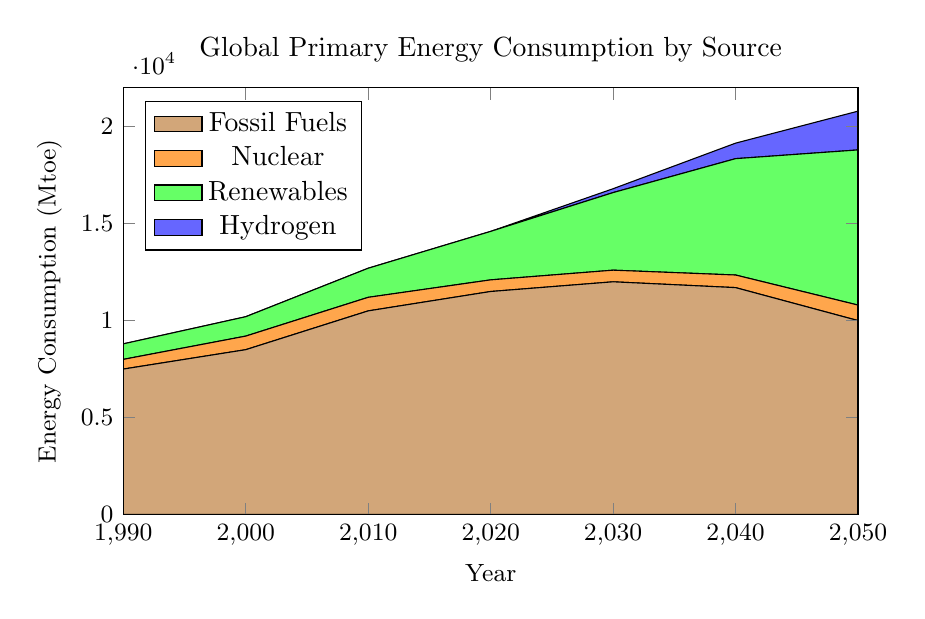
\begin{tikzpicture}
\begin{axis}[
    width=0.9\textwidth,
    height=7cm,
    xlabel={Year},
    ylabel={Energy Consumption (Mtoe)},
    title={Global Primary Energy Consumption by Source},
    legend pos=north west,
    stack plots=y,
    area style,
    xmin=1990, xmax=2050,
    ymin=0, ymax=22000,
    xtick={1990,2000,2010,2020,2030,2040,2050},
    label style={font=\small},
    tick label style={font=\small}
]
\addplot[fill=brown!70] coordinates
    {(1990,7500)(2000,8500)(2010,10500)(2020,11500)(2030,12000)(2040,11700)(2050,10000)}
    \closedcycle;
\addplot[fill=orange!70] coordinates
    {(1990,500)(2000,700)(2010,700)(2020,600)(2030,600)(2040,650)(2050,800)}
    \closedcycle;
\addplot[fill=green!60] coordinates
    {(1990,800)(2000,1000)(2010,1500)(2020,2500)(2030,4000)(2040,6000)(2050,8000)}
    \closedcycle;
\addplot[fill=blue!60] coordinates
    {(1990,0)(2000,0)(2010,0)(2020,0)(2030,200)(2040,800)(2050,2000)}
    \closedcycle;
\legend{Fossil Fuels, Nuclear, Renewables, Hydrogen}
\end{axis}
\end{tikzpicture}%
}

\newcommand{\smrtempfigure}{%
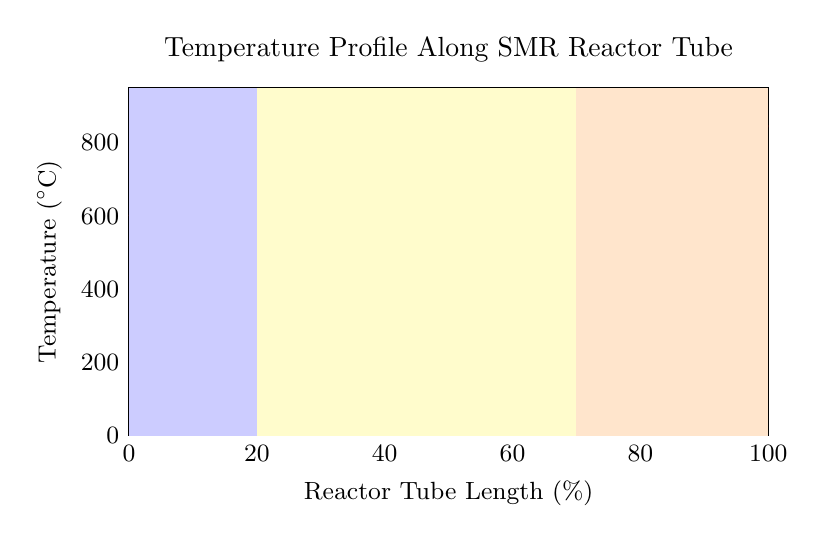
\begin{tikzpicture}
\begin{axis}[
    width=0.8\textwidth,
    height=6cm,
    xlabel={Reactor Tube Length (\%)},
    ylabel={Temperature (\unitdegree)},
    title={Temperature Profile Along SMR Reactor Tube},
    grid=major,
    xmin=0, xmax=100,
    ymin=0, ymax=950,
    label style={font=\small},
    tick label style={font=\small}
]
\addplot[thick, red, domain=0:100, samples=100]
    {600 + 250 * (1 - exp(-x/25))};
\addplot[fill=blue!20, draw=none, domain=0:20, samples=2] {950} \closedcycle;
\addplot[fill=yellow!20, draw=none, domain=20:70, samples=2] {950} \closedcycle;
\addplot[fill=orange!20, draw=none, domain=70:100, samples=2] {950} \closedcycle;
\end{axis}
\end{tikzpicture}%
}

\newcommand{\polarizationfigure}{%
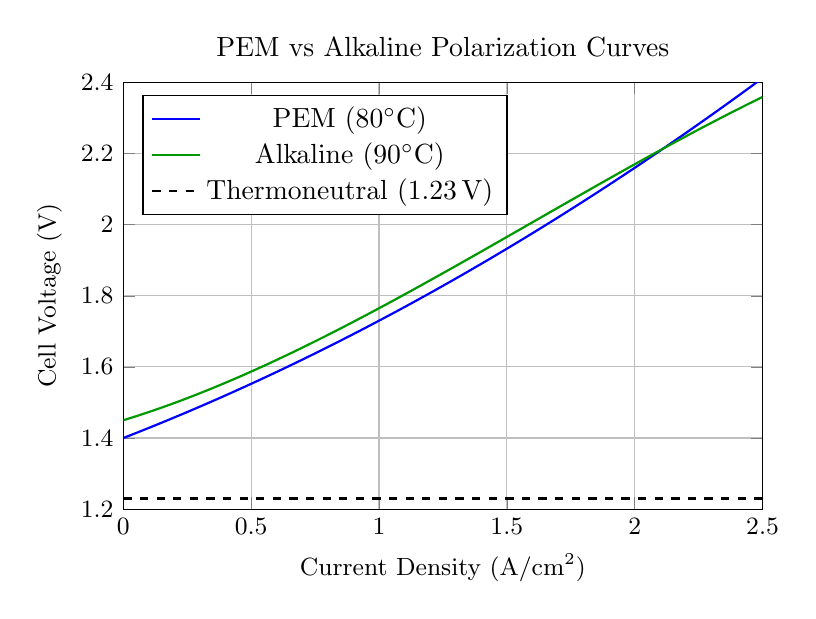
\begin{tikzpicture}
\begin{axis}[
    width=0.8\textwidth,
    height=7cm,
    xlabel={Current Density (A/cm$^2$)},
    ylabel={Cell Voltage (V)},
    title={PEM vs Alkaline Polarization Curves},
    grid=major,
    xmin=0, xmax=2.5,
    ymin=1.2, ymax=2.4,
    legend pos=north west,
    label style={font=\small},
    tick label style={font=\small}
]
\addplot[thick, blue, domain=0:2.5, samples=80]
    {1.4 + 0.28*x + 0.05*x^2};
\addplot[thick, green!60!black, domain=0:2.5, samples=80]
    {1.45 + 0.22*x + 0.12*x^2 - 0.025*x^3};
\addplot[thick, black, dashed, domain=0:2.5, samples=2] {1.23};
\legend{PEM (80\unitdegree), Alkaline (90\unitdegree), Thermoneutral (1.23\,V)}
\end{axis}
\end{tikzpicture}%
}

% --- Volume II figures ---

\newcommand{\cngcompressionfigure}{%
\resizebox{0.98\textwidth}{!}{%
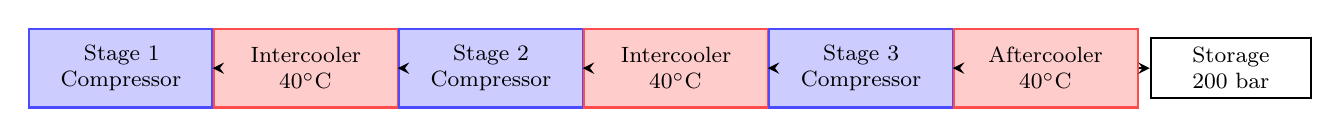
\begin{tikzpicture}[node distance=2.35cm, auto, font=\footnotesize]
    \tikzset{
        comp/.style={rectangle, draw=blue!70, thick, fill=blue!20,
                     text width=2.1cm, align=center, minimum height=1cm},
        cooler/.style={rectangle, draw=red!70, thick, fill=red!20,
                       text width=2.1cm, align=center, minimum height=1cm},
        arrow/.style={thick, ->, >=stealth}
    }
    \node[comp]   (c1)      {Stage 1\\Compressor};
    \node[cooler, right of=c1]  (cool1)  {Intercooler\\40\unitdegree};
    \node[comp,   right of=cool1] (c2)   {Stage 2\\Compressor};
    \node[cooler, right of=c2]  (cool2)  {Intercooler\\40\unitdegree};
    \node[comp,   right of=cool2] (c3)   {Stage 3\\Compressor};
    \node[cooler, right of=c3]  (cool3)  {Aftercooler\\40\unitdegree};
    \node[rectangle, draw, thick, right of=cool3, text width=1.8cm, align=center]
        (storage) {Storage\\200 bar};
    \draw[arrow] (c1) -- (cool1);
    \draw[arrow] (cool1) -- (c2);
    \draw[arrow] (c2) -- (cool2);
    \draw[arrow] (cool2) -- (c3);
    \draw[arrow] (c3) -- (cool3);
    \draw[arrow] (cool3) -- (storage);
\end{tikzpicture}}%
}

% --- Volume III figures ---

\newcommand{\lcohfigure}{%
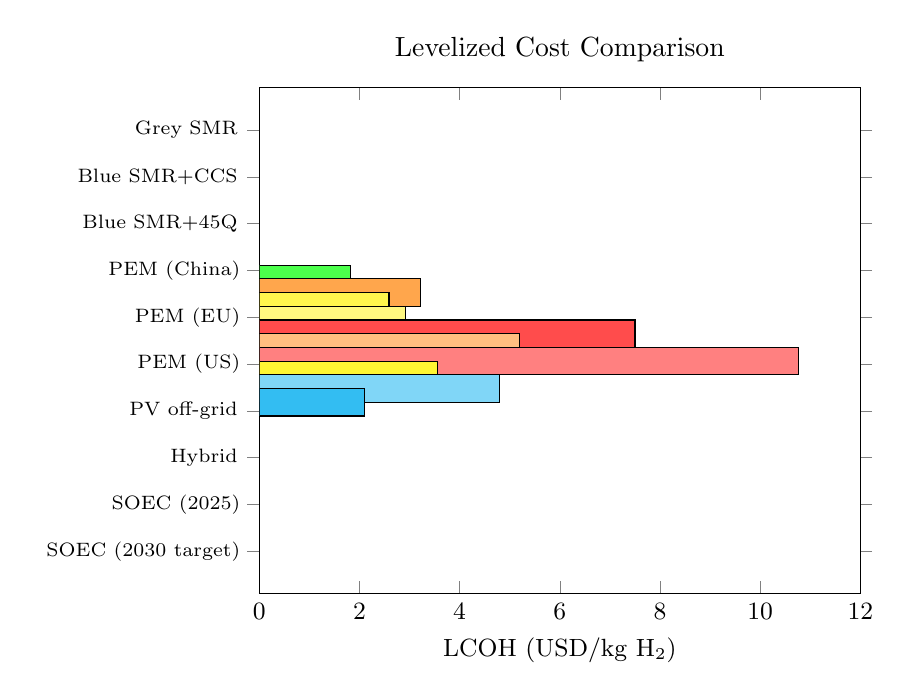
\begin{tikzpicture}
\begin{axis}[
    width=0.76\textwidth,
    height=8cm,
    xlabel={LCOH (USD/kg H$_2$)},
    ytick={1,2,3,4,5,6,7,8,9,10},
    yticklabels={Grey SMR, Blue SMR+CCS, Blue SMR+45Q, PEM (China),
                 PEM (EU), PEM (US), PV off-grid, Hybrid,
                 SOEC (2025), SOEC (2030 target)},
    title={Levelized Cost Comparison},
    xmin=0, xmax=12,
    y dir=reverse,
    xbar,
    bar width=0.35cm,
    label style={font=\small},
    tick label style={font=\small},
    yticklabel style={font=\scriptsize, text width=2.55cm, align=right}
]
\addplot[fill=green!70]  coordinates {(1.82,1)};
\addplot[fill=orange!70] coordinates {(3.22,2)};
\addplot[fill=yellow!70] coordinates {(2.59,3)};
\addplot[fill=yellow!50] coordinates {(2.92,4)};
\addplot[fill=red!70]    coordinates {(7.50,5)};
\addplot[fill=orange!50] coordinates {(5.20,6)};
\addplot[fill=red!50]    coordinates {(10.77,7)};
\addplot[fill=yellow!80] coordinates {(3.55,8)};
\addplot[fill=cyan!50]   coordinates {(4.80,9)};
\addplot[fill=cyan!80]   coordinates {(2.10,10)};
\end{axis}
\end{tikzpicture}%
}

\newcommand{\economyscale}{%
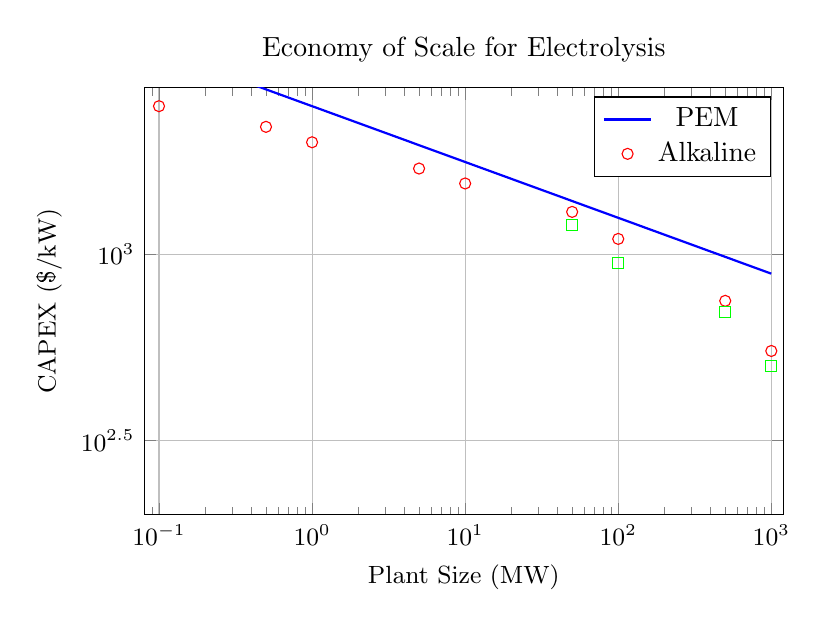
\begin{tikzpicture}
\begin{loglogaxis}[
    width=0.8\textwidth,
    height=7cm,
    xlabel={Plant Size (MW)},
    ylabel={CAPEX (\$/kW)},
    title={Economy of Scale for Electrolysis},
    grid=major,
    xmin=0.08, xmax=1200,
    ymin=200, ymax=2800,
    label style={font=\small},
    tick label style={font=\small}
]
\addplot[thick, blue, domain=0.1:1000, samples=60]
    {2500 * x^(-0.15)};
\addplot[only marks, red, mark=o] coordinates {
    (0.1,2500)(0.5,2200)(1,2000)(5,1700)(10,1550)
    (50,1300)(100,1100)(500,750)(1000,550)
};
\addplot[only marks, green, mark=square] coordinates {
    (50,1200)(100,950)(500,700)(1000,500)
};
\legend{PEM, Alkaline}
\end{loglogaxis}
\end{tikzpicture}%
}

\newcommand{\tornadofigure}{%
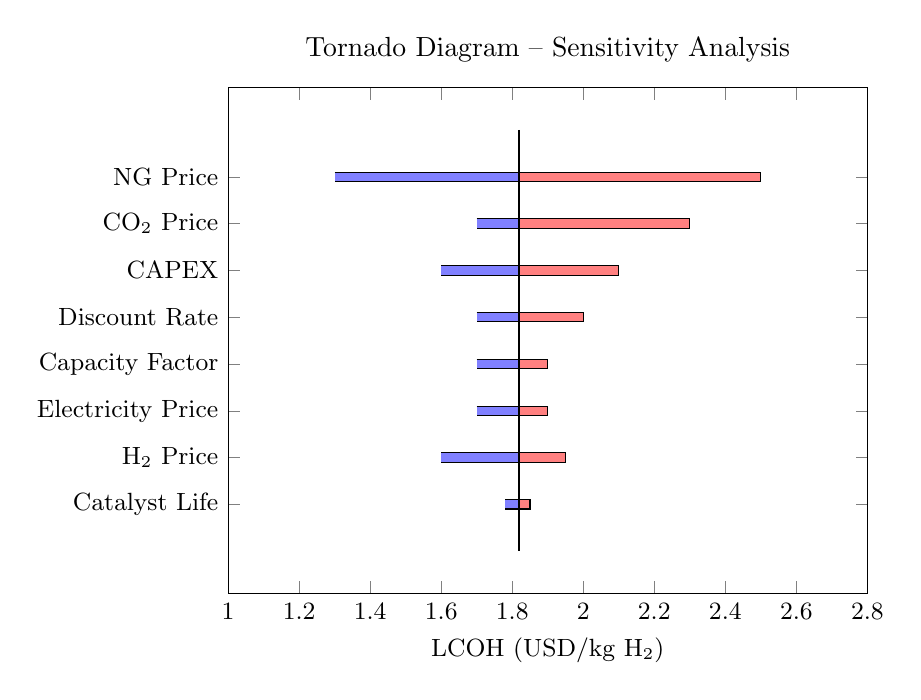
\begin{tikzpicture}
\begin{axis}[
    width=0.8\textwidth,
    height=8cm,
    xlabel={LCOH (USD/kg H$_2$)},
    ytick={1,2,3,4,5,6,7,8},
    yticklabels={NG Price, CO$_2$ Price, CAPEX, Discount Rate,
                 Capacity Factor, Electricity Price, H$_2$ Price, Catalyst Life},
    title={Tornado Diagram -- Sensitivity Analysis},
    xmin=1.0, xmax=2.8,
    y dir=reverse,
    label style={font=\small},
    tick label style={font=\small}
]
\addplot[fill=blue!50]  coordinates {(1.30,0.9)(1.82,0.9)(1.82,1.1)(1.30,1.1)};
\addplot[fill=red!50]   coordinates {(1.82,0.9)(2.50,0.9)(2.50,1.1)(1.82,1.1)};
\addplot[fill=blue!50]  coordinates {(1.70,1.9)(1.82,1.9)(1.82,2.1)(1.70,2.1)};
\addplot[fill=red!50]   coordinates {(1.82,1.9)(2.30,1.9)(2.30,2.1)(1.82,2.1)};
\addplot[fill=blue!50]  coordinates {(1.60,2.9)(1.82,2.9)(1.82,3.1)(1.60,3.1)};
\addplot[fill=red!50]   coordinates {(1.82,2.9)(2.10,2.9)(2.10,3.1)(1.82,3.1)};
\addplot[fill=blue!50]  coordinates {(1.70,3.9)(1.82,3.9)(1.82,4.1)(1.70,4.1)};
\addplot[fill=red!50]   coordinates {(1.82,3.9)(2.00,3.9)(2.00,4.1)(1.82,4.1)};
\addplot[fill=blue!50]  coordinates {(1.70,4.9)(1.82,4.9)(1.82,5.1)(1.70,5.1)};
\addplot[fill=red!50]   coordinates {(1.82,4.9)(1.90,4.9)(1.90,5.1)(1.82,5.1)};
\addplot[fill=blue!50]  coordinates {(1.70,5.9)(1.82,5.9)(1.82,6.1)(1.70,6.1)};
\addplot[fill=red!50]   coordinates {(1.82,5.9)(1.90,5.9)(1.90,6.1)(1.82,6.1)};
\addplot[fill=blue!50]  coordinates {(1.60,6.9)(1.82,6.9)(1.82,7.1)(1.60,7.1)};
\addplot[fill=red!50]   coordinates {(1.82,6.9)(1.95,6.9)(1.95,7.1)(1.82,7.1)};
\addplot[fill=blue!50]  coordinates {(1.78,7.9)(1.82,7.9)(1.82,8.1)(1.78,8.1)};
\addplot[fill=red!50]   coordinates {(1.82,7.9)(1.85,7.9)(1.85,8.1)(1.82,8.1)};
\addplot[black, thick]  coordinates {(1.82,0)(1.82,9)};
\end{axis}
\end{tikzpicture}%
}

\newcommand{\mcdaradar}{%
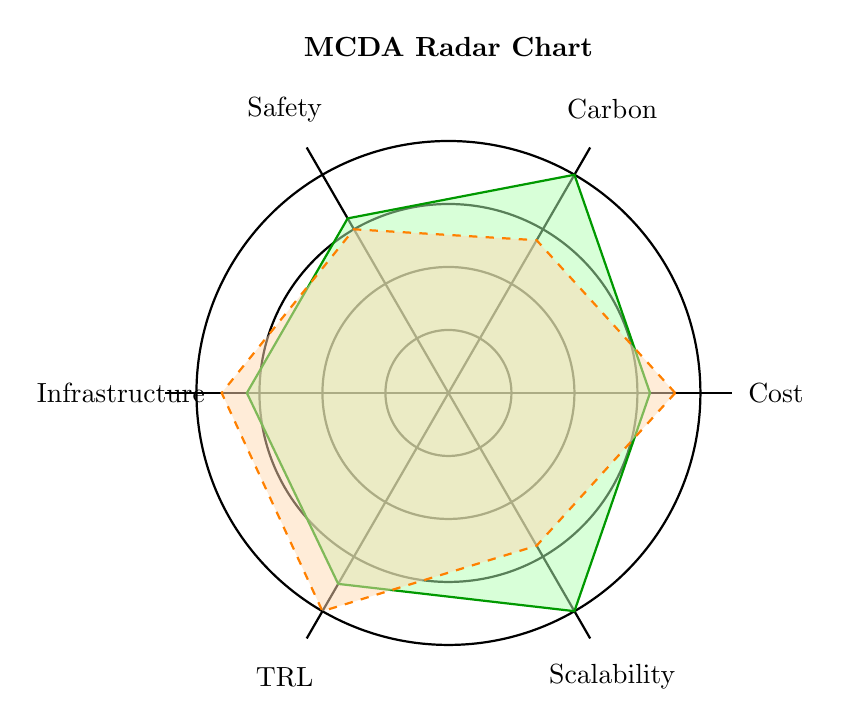
\begin{tikzpicture}[scale=0.8]
\draw[thick] (0,0) circle (4cm);
\draw[thick] (0,0) circle (3cm);
\draw[thick] (0,0) circle (2cm);
\draw[thick] (0,0) circle (1cm);
\foreach \angle/\label in {
    0/Cost, 60/Carbon, 120/Safety,
    180/Infrastructure, 240/TRL, 300/Scalability}{
    \draw[thick] (0,0) -- (\angle:4.5cm);
    \node at (\angle:5.2cm) {\label};
}
\fill[green!30, opacity=0.5]
    (0:3.2cm) -- (60:4.0cm) -- (120:3.2cm) --
    (180:3.2cm) -- (240:3.5cm) -- (300:4.0cm) -- cycle;
\draw[thick, green!60!black]
    (0:3.2cm) -- (60:4.0cm) -- (120:3.2cm) --
    (180:3.2cm) -- (240:3.5cm) -- (300:4.0cm) -- cycle;
\fill[orange!30, opacity=0.5]
    (0:3.6cm) -- (60:2.8cm) -- (120:3.0cm) --
    (180:3.6cm) -- (240:4.0cm) -- (300:2.8cm) -- cycle;
\draw[thick, orange, dashed]
    (0:3.6cm) -- (60:2.8cm) -- (120:3.0cm) --
    (180:3.6cm) -- (240:4.0cm) -- (300:2.8cm) -- cycle;
\node at (0,5.5) {\textbf{MCDA Radar Chart}};
\end{tikzpicture}%
}

% --- NEW FIGURES ---

\newcommand{\lcaflowchart}{%
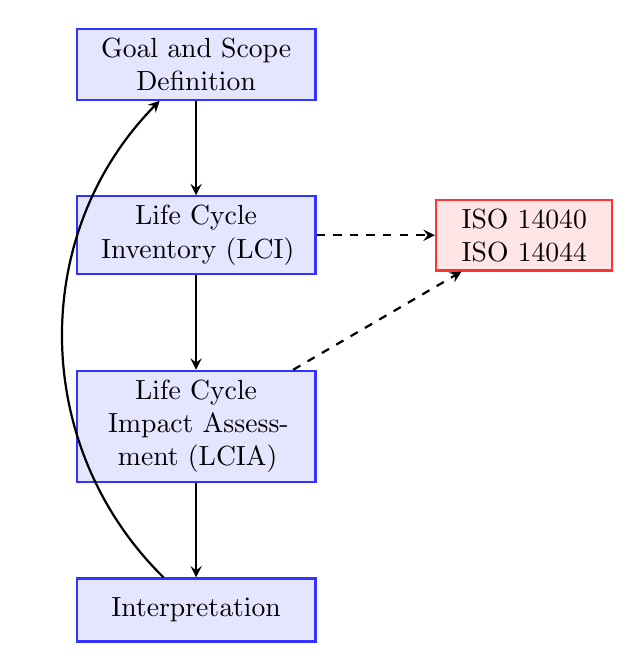
\begin{tikzpicture}[node distance=1.2cm]
    \tikzset{
        block/.style={rectangle, draw=blue!80, thick, fill=blue!10,
                     text width=2.8cm, align=center, minimum height=0.8cm},
        arrow/.style={thick, ->, >=stealth}
    }
    \node[block] (goal) {Goal and Scope Definition};
    \node[block, below=of goal] (inventory) {Life Cycle Inventory (LCI)};
    \node[block, below=of inventory] (impact) {Life Cycle Impact Assessment (LCIA)};
    \node[block, below=of impact] (interpretation) {Interpretation};
    \draw[arrow] (goal) -- (inventory);
    \draw[arrow] (inventory) -- (impact);
    \draw[arrow] (impact) -- (interpretation);
    \draw[arrow, bend left=45] (interpretation) to (goal);
    \node[rectangle, draw=red!80, thick, fill=red!10, right=1.5cm of inventory,
         text width=2cm, align=center] (iso) {ISO 14040\\ISO 14044};
    \draw[arrow, dashed] (inventory) -- (iso);
    \draw[arrow, dashed] (impact) -- (iso);
\end{tikzpicture}%
}

\newcommand{\aspenSMRmodel}{%
\resizebox{0.98\textwidth}{!}{%
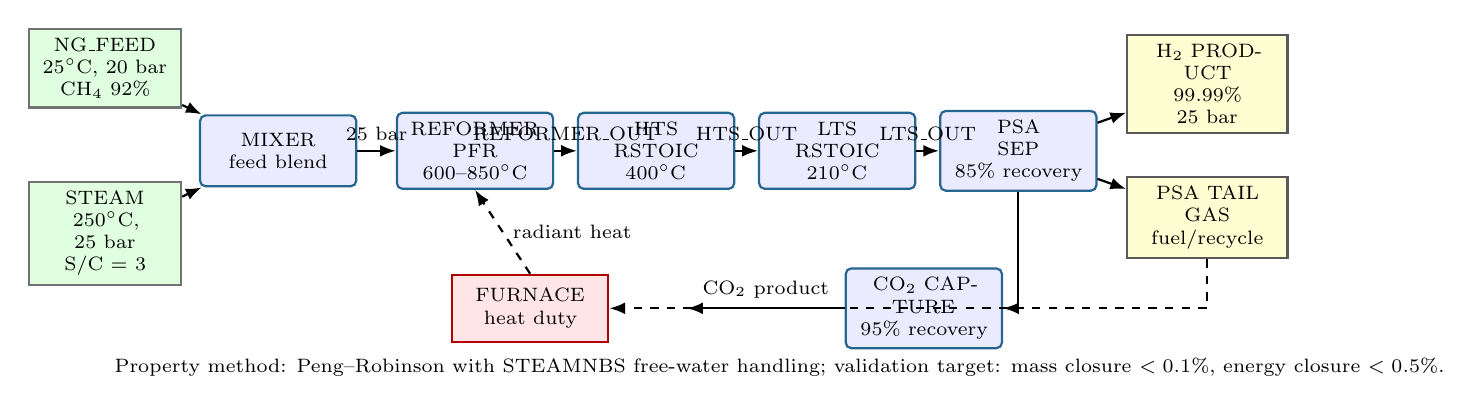
\begin{tikzpicture}[font=\scriptsize]
    \tikzset{
        modelblock/.style={rectangle, rounded corners=2pt, draw=HeadingBlue!85,
            thick, fill=blue!8, minimum width=1.85cm, minimum height=0.9cm,
            text width=1.75cm, align=center},
        feed/.style={rectangle, draw=black!55, thick, fill=green!12,
            minimum width=1.8cm, minimum height=0.85cm, text width=1.7cm,
            align=center},
        product/.style={rectangle, draw=black!65, thick, fill=yellow!18,
            minimum width=1.9cm, minimum height=0.85cm, text width=1.8cm,
            align=center},
        utility/.style={rectangle, draw=red!70!black, thick, fill=red!10,
            minimum width=1.85cm, minimum height=0.85cm, text width=1.75cm,
            align=center},
        modelstream/.style={thick, -{Latex[length=2mm]}},
        utilstream/.style={thick, dashed, -{Latex[length=2mm]}}
    }
    \node[feed] (ng) at (0,1.05) {NG\_FEED\\25\unitdegree, 20 bar\\CH$_4$ 92\%};
    \node[feed] (steam) at (0,-1.05) {STEAM\\250\unitdegree, 25 bar\\S/C = 3};
    \node[modelblock] (mix) at (2.2,0) {MIXER\\feed blend};
    \node[modelblock] (reformer) at (4.7,0) {REFORMER\\PFR\\600--850\unitdegree};
    \node[modelblock] (hts) at (7.0,0) {HTS\\RSTOIC\\400\unitdegree};
    \node[modelblock] (lts) at (9.3,0) {LTS\\RSTOIC\\210\unitdegree};
    \node[modelblock] (psa) at (11.6,0) {PSA\\SEP\\85\% recovery};
    \node[product] (h2prod) at (14.0,0.85) {H$_2$ PRODUCT\\99.99\%\\25 bar};
    \node[product] (tail) at (14.0,-0.85) {PSA TAIL GAS\\fuel/recycle};
    \node[modelblock] (capture) at (10.4,-2.0) {CO$_2$ CAPTURE\\95\% recovery};
    \node[utility] (furnace) at (5.4,-2.0) {FURNACE\\heat duty};
    \draw[modelstream] (ng) -- (mix);
    \draw[modelstream] (steam) -- (mix);
    \draw[modelstream] (mix) -- node[above] {25 bar} (reformer);
    \draw[modelstream] (reformer) -- node[above] {REFORMER\_OUT} (hts);
    \draw[modelstream] (hts) -- node[above] {HTS\_OUT} (lts);
    \draw[modelstream] (lts) -- node[above] {LTS\_OUT} (psa);
    \draw[modelstream] (psa) -- (h2prod);
    \draw[modelstream] (psa) -- (tail);
    \draw[modelstream] (psa.south) |- (capture.east);
    \draw[modelstream] (capture.west) -- node[above] {CO$_2$ product} ++(-2.0,0);
    \draw[utilstream] (tail.south) |- (furnace.east);
    \draw[utilstream] (furnace.north) -- node[right] {radiant heat} (reformer.south);
    \node[anchor=west, font=\scriptsize] at (0,-2.75)
        {Property method: Peng--Robinson with STEAMNBS free-water handling; validation target: mass closure $<0.1\%$, energy closure $<0.5\%$.};
\end{tikzpicture}}%
}

\newcommand{\aspenCNGmodel}{%
\resizebox{0.98\textwidth}{!}{%
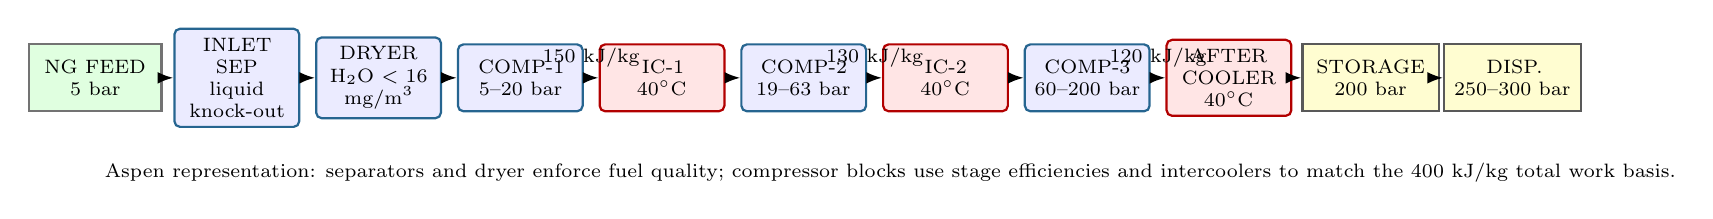
\begin{tikzpicture}[font=\scriptsize]
    \tikzset{
        gasblock/.style={rectangle, rounded corners=2pt, draw=HeadingBlue!85,
            thick, fill=blue!8, minimum width=1.45cm, minimum height=0.85cm,
            text width=1.35cm, align=center},
        coolblock/.style={rectangle, rounded corners=2pt, draw=red!70!black,
            thick, fill=red!10, minimum width=1.45cm, minimum height=0.85cm,
            text width=1.35cm, align=center},
        feed/.style={rectangle, draw=black!55, thick, fill=green!12,
            minimum width=1.55cm, minimum height=0.85cm, text width=1.45cm,
            align=center},
        product/.style={rectangle, draw=black!65, thick, fill=yellow!18,
            minimum width=1.6cm, minimum height=0.85cm, text width=1.5cm,
            align=center},
        stream/.style={thick, -{Latex[length=2mm]}}
    }
    \node[feed] (ng) at (0,0) {NG FEED\\5 bar};
    \node[gasblock] (sep) at (1.8,0) {INLET SEP\\liquid knock-out};
    \node[gasblock] (dryer) at (3.6,0) {DRYER\\H$_2$O $<16$ mg/m$^3$};
    \node[gasblock] (c1) at (5.4,0) {COMP-1\\5--20 bar};
    \node[coolblock] (ic1) at (7.2,0) {IC-1\\40\unitdegree};
    \node[gasblock] (c2) at (9.0,0) {COMP-2\\19--63 bar};
    \node[coolblock] (ic2) at (10.8,0) {IC-2\\40\unitdegree};
    \node[gasblock] (c3) at (12.6,0) {COMP-3\\60--200 bar};
    \node[coolblock] (ac) at (14.4,0) {AFTER\\COOLER\\40\unitdegree};
    \node[product] (store) at (16.2,0) {STORAGE\\200 bar};
    \node[product] (disp) at (18.0,0) {DISP.\\250--300 bar};
    \draw[stream] (ng) -- (sep);
    \draw[stream] (sep) -- (dryer);
    \draw[stream] (dryer) -- (c1);
    \draw[stream] (c1) -- node[above] {150 kJ/kg} (ic1);
    \draw[stream] (ic1) -- (c2);
    \draw[stream] (c2) -- node[above] {130 kJ/kg} (ic2);
    \draw[stream] (ic2) -- (c3);
    \draw[stream] (c3) -- node[above] {120 kJ/kg} (ac);
    \draw[stream] (ac) -- (store);
    \draw[stream] (store) -- (disp);
    \node[anchor=west, font=\scriptsize] at (0,-1.2)
        {Aspen representation: separators and dryer enforce fuel quality; compressor blocks use stage efficiencies and intercoolers to match the 400 kJ/kg total work basis.};
\end{tikzpicture}}%
}

\newcommand{\aspenElectrolysismodel}{%
\resizebox{0.98\textwidth}{!}{%
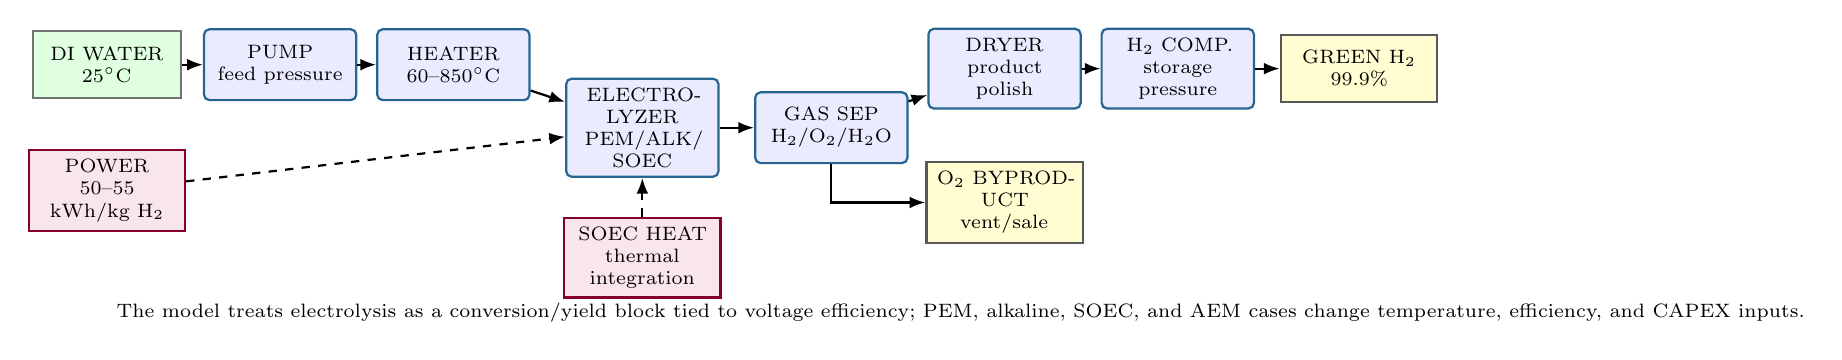
\begin{tikzpicture}[font=\scriptsize]
    \tikzset{
        modelblock/.style={rectangle, rounded corners=2pt, draw=HeadingBlue!85,
            thick, fill=blue!8, minimum width=1.8cm, minimum height=0.9cm,
            text width=1.7cm, align=center},
        feed/.style={rectangle, draw=black!55, thick, fill=green!12,
            minimum width=1.75cm, minimum height=0.85cm, text width=1.65cm,
            align=center},
        product/.style={rectangle, draw=black!65, thick, fill=yellow!18,
            minimum width=1.85cm, minimum height=0.85cm, text width=1.75cm,
            align=center},
        utility/.style={rectangle, draw=purple!70!black, thick, fill=purple!10,
            minimum width=1.85cm, minimum height=0.85cm, text width=1.75cm,
            align=center},
        stream/.style={thick, -{Latex[length=2mm]}},
        utilstream/.style={thick, dashed, -{Latex[length=2mm]}}
    }
    \node[feed] (water) at (0,0.8) {DI WATER\\25\unitdegree};
    \node[utility] (power) at (0,-0.8) {POWER\\50--55 kWh/kg H$_2$};
    \node[modelblock] (pump) at (2.2,0.8) {PUMP\\feed pressure};
    \node[modelblock] (heat) at (4.4,0.8) {HEATER\\60--850\unitdegree};
    \node[modelblock] (electro) at (6.8,0) {ELECTRO-\\LYZER\\PEM/ALK/\\SOEC};
    \node[modelblock] (sep) at (9.2,0) {GAS SEP\\H$_2$/O$_2$/H$_2$O};
    \node[modelblock] (dryer) at (11.4,0.75) {DRYER\\product polish};
    \node[modelblock] (comp) at (13.6,0.75) {H$_2$ COMP.\\storage pressure};
    \node[product] (h2) at (15.9,0.75) {GREEN H$_2$\\99.9\%};
    \node[product] (o2) at (11.4,-0.95) {O$_2$ BYPRODUCT\\vent/sale};
    \node[utility] (heatint) at (6.8,-1.65) {SOEC HEAT\\thermal integration};
    \draw[stream] (water) -- (pump);
    \draw[stream] (pump) -- (heat);
    \draw[stream] (heat) -- (electro);
    \draw[utilstream] (power) -- (electro);
    \draw[utilstream] (heatint) -- (electro);
    \draw[stream] (electro) -- (sep);
    \draw[stream] (sep) -- (dryer);
    \draw[stream] (dryer) -- (comp);
    \draw[stream] (comp) -- (h2);
    \draw[stream] (sep.south) |- (o2.west);
    \node[anchor=west, font=\scriptsize] at (0,-2.35)
        {The model treats electrolysis as a conversion/yield block tied to voltage efficiency; PEM, alkaline, SOEC, and AEM cases change temperature, efficiency, and CAPEX inputs.};
\end{tikzpicture}}%
}

\newcommand{\aspenMethanolmodel}{%
\resizebox{0.98\textwidth}{!}{%
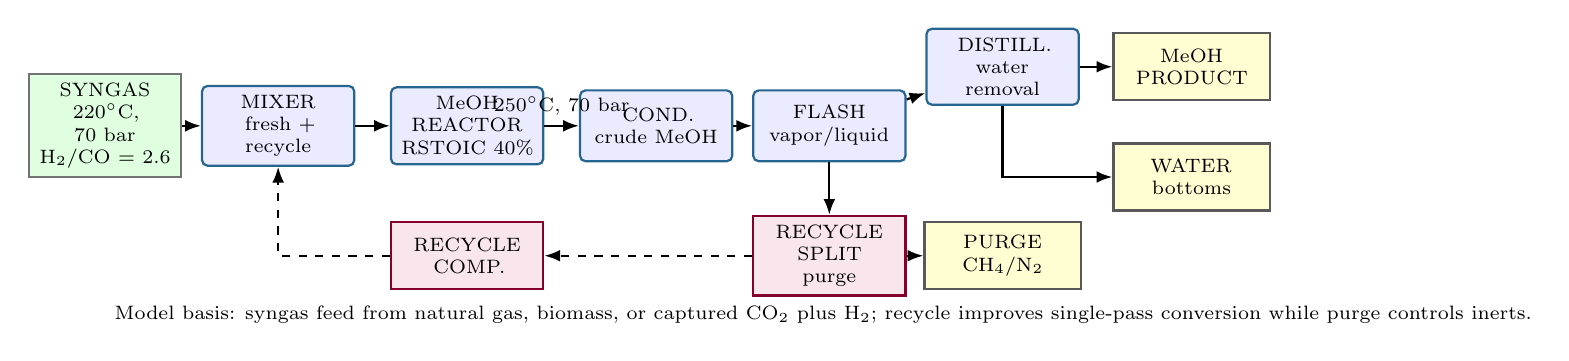
\begin{tikzpicture}[font=\scriptsize]
    \tikzset{
        modelblock/.style={rectangle, rounded corners=2pt, draw=HeadingBlue!85,
            thick, fill=blue!8, minimum width=1.8cm, minimum height=0.9cm,
            text width=1.7cm, align=center},
        feed/.style={rectangle, draw=black!55, thick, fill=green!12,
            minimum width=1.8cm, minimum height=0.85cm, text width=1.7cm,
            align=center},
        product/.style={rectangle, draw=black!65, thick, fill=yellow!18,
            minimum width=1.85cm, minimum height=0.85cm, text width=1.75cm,
            align=center},
        recycle/.style={rectangle, draw=purple!70!black, thick, fill=purple!10,
            minimum width=1.8cm, minimum height=0.85cm, text width=1.7cm,
            align=center},
        stream/.style={thick, -{Latex[length=2mm]}},
        recyclestream/.style={thick, dashed, -{Latex[length=2mm]}}
    }
    \node[feed] (syngas) at (0,0) {SYNGAS\\220\unitdegree, 70 bar\\H$_2$/CO = 2.6};
    \node[modelblock] (mix) at (2.2,0) {MIXER\\fresh + recycle};
    \node[modelblock] (reactor) at (4.6,0) {MeOH\\REACTOR\\RSTOIC 40\%};
    \node[modelblock] (cond) at (7.0,0) {COND.\\crude MeOH};
    \node[modelblock] (flash) at (9.2,0) {FLASH\\vapor/liquid};
    \node[modelblock] (dist) at (11.4,0.75) {DISTILL.\\water removal};
    \node[product] (prod) at (13.8,0.75) {MeOH\\PRODUCT};
    \node[product] (water) at (13.8,-0.65) {WATER\\bottoms};
    \node[recycle] (split) at (9.2,-1.65) {RECYCLE\\SPLIT\\purge};
    \node[recycle] (rcomp) at (4.6,-1.65) {RECYCLE\\COMP.};
    \node[product] (purge) at (11.4,-1.65) {PURGE\\CH$_4$/N$_2$};
    \draw[stream] (syngas) -- (mix);
    \draw[stream] (mix) -- (reactor);
    \draw[stream] (reactor) -- node[above] {250\unitdegree, 70 bar} (cond);
    \draw[stream] (cond) -- (flash);
    \draw[stream] (flash) -- (dist);
    \draw[stream] (dist) -- (prod);
    \draw[stream] (dist.south) |- (water.west);
    \draw[stream] (flash.south) -- (split.north);
    \draw[stream] (split) -- (purge);
    \draw[recyclestream] (split.west) -- (rcomp.east);
    \draw[recyclestream] (rcomp.west) -| (mix.south);
    \node[anchor=west, font=\scriptsize] at (0,-2.4)
        {Model basis: syngas feed from natural gas, biomass, or captured CO$_2$ plus H$_2$; recycle improves single-pass conversion while purge controls inerts.};
\end{tikzpicture}}%
}

\newcommand{\soecfigure}{%
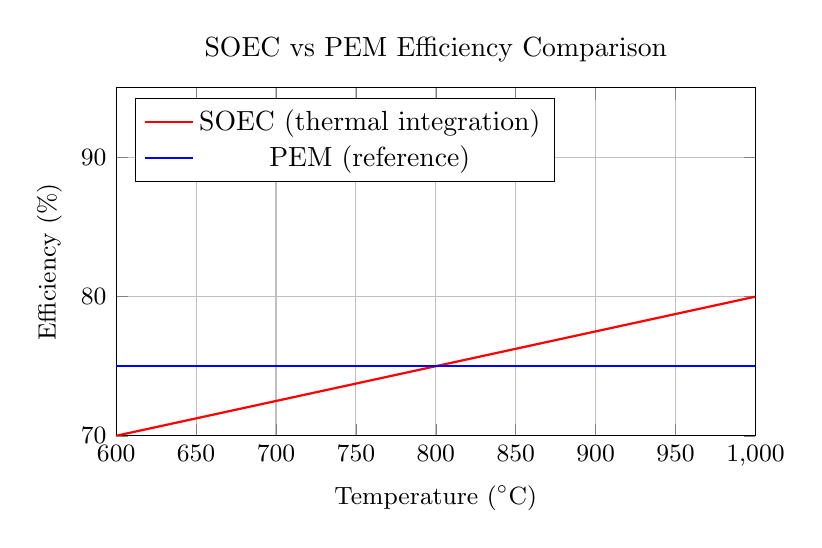
\begin{tikzpicture}
\begin{axis}[
    width=0.8\textwidth,
    height=6cm,
    xlabel={Temperature (\unitdegree)},
    ylabel={Efficiency (\%)},
    title={SOEC vs PEM Efficiency Comparison},
    grid=major,
    xmin=600, xmax=1000,
    ymin=70, ymax=95,
    legend pos=north west,
    label style={font=\small},
    tick label style={font=\small}
]
\addplot[thick, red, domain=600:1000, samples=50]
    {70 + 0.025*(x-600)};
\addplot[thick, blue, domain=600:1000, samples=2]
    {75};
\legend{SOEC (thermal integration), PEM (reference)}
\end{axis}
\end{tikzpicture}%
}

\newcommand{\africafigure}{%
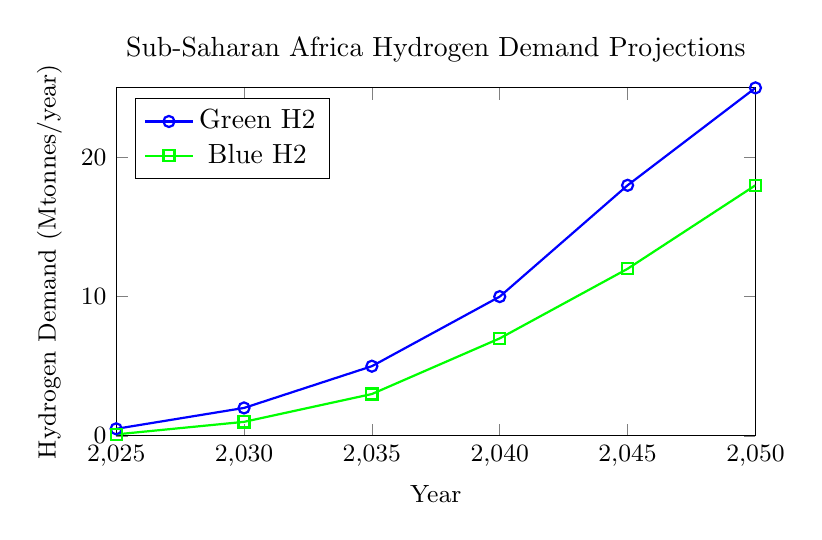
\begin{tikzpicture}
\begin{axis}[
    width=0.8\textwidth,
    height=6cm,
    xlabel={Year},
    ylabel={Hydrogen Demand (Mtonnes/year)},
    title={Sub-Saharan Africa Hydrogen Demand Projections},
    legend pos=north west,
    xmin=2025, xmax=2050,
    ymin=0, ymax=25,
    label style={font=\small},
    tick label style={font=\small}
]
\addplot[thick, blue, mark=o] coordinates
    {(2025,0.5)(2030,2.0)(2035,5.0)(2040,10.0)(2045,18.0)(2050,25.0)};
\addplot[thick, green, mark=square] coordinates
    {(2025,0.1)(2030,1.0)(2035,3.0)(2040,7.0)(2045,12.0)(2050,18.0)};
\legend{Green H2, Blue H2}
\end{axis}
\end{tikzpicture}%
}

\newcommand{\costcarbonmapfigure}{%
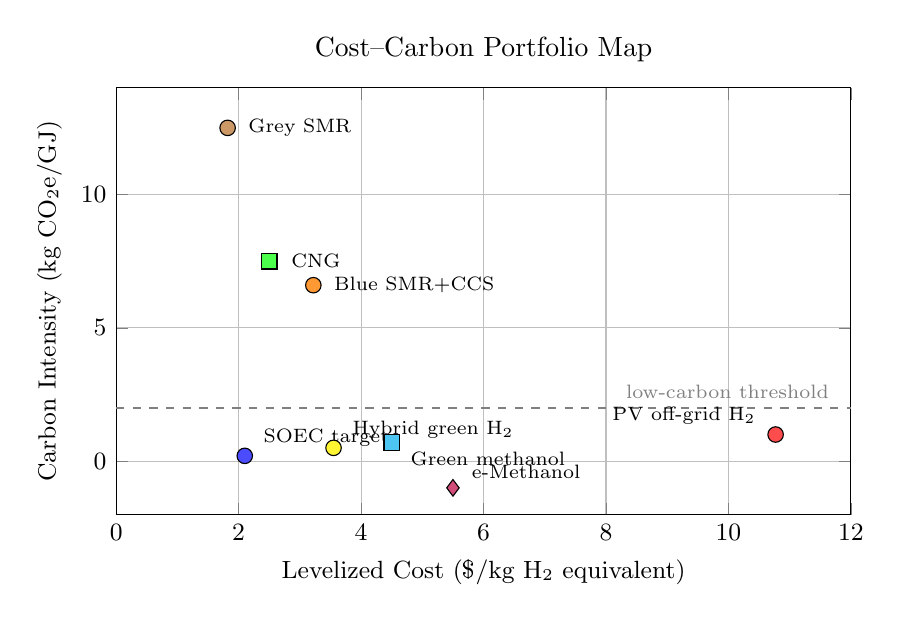
\begin{tikzpicture}
\begin{axis}[
    width=0.9\textwidth,
    height=7cm,
    xlabel={Levelized Cost (\$/kg H$_2$ equivalent)},
    ylabel={Carbon Intensity (kg CO$_2$e/GJ)},
    title={Cost--Carbon Portfolio Map},
    xmin=0, xmax=12,
    ymin=-2, ymax=14,
    grid=both,
    label style={font=\small},
    tick label style={font=\small}
]
\addplot[gray, dashed, thick] coordinates {(0,2)(12,2)};
\node[font=\scriptsize, anchor=south east, text=gray] at (axis cs:11.8,2) {low-carbon threshold};

\addplot[only marks, mark=*, mark size=2.8pt, fill=brown!80, draw=black] coordinates {(1.82,12.5)};
\node[font=\scriptsize, anchor=west] at (axis cs:2.0,12.5) {Grey SMR};
\addplot[only marks, mark=*, mark size=2.8pt, fill=orange!80, draw=black] coordinates {(3.22,6.6)};
\node[font=\scriptsize, anchor=west] at (axis cs:3.4,6.6) {Blue SMR+CCS};
\addplot[only marks, mark=*, mark size=2.8pt, fill=yellow!80, draw=black] coordinates {(3.55,0.5)};
\node[font=\scriptsize, anchor=south west] at (axis cs:3.7,0.5) {Hybrid green H$_2$};
\addplot[only marks, mark=*, mark size=2.8pt, fill=red!70, draw=black] coordinates {(10.77,1.0)};
\node[font=\scriptsize, anchor=south east] at (axis cs:10.6,1.0) {PV off-grid H$_2$};
\addplot[only marks, mark=*, mark size=2.8pt, fill=blue!70, draw=black] coordinates {(2.10,0.2)};
\node[font=\scriptsize, anchor=south west] at (axis cs:2.25,0.2) {SOEC target};
\addplot[only marks, mark=square*, mark size=2.8pt, fill=green!70, draw=black] coordinates {(2.50,7.5)};
\node[font=\scriptsize, anchor=west] at (axis cs:2.7,7.5) {CNG};
\addplot[only marks, mark=square*, mark size=2.8pt, fill=cyan!70, draw=black] coordinates {(4.50,0.7)};
\node[font=\scriptsize, anchor=north west] at (axis cs:4.65,0.7) {Green methanol};
\addplot[only marks, mark=diamond*, mark size=3pt, fill=purple!70, draw=black] coordinates {(5.50,-1.0)};
\node[font=\scriptsize, anchor=south west] at (axis cs:5.65,-1.0) {e-Methanol};
\end{axis}
\end{tikzpicture}%
}

\newcommand{\costtrajectoryfigure}{%
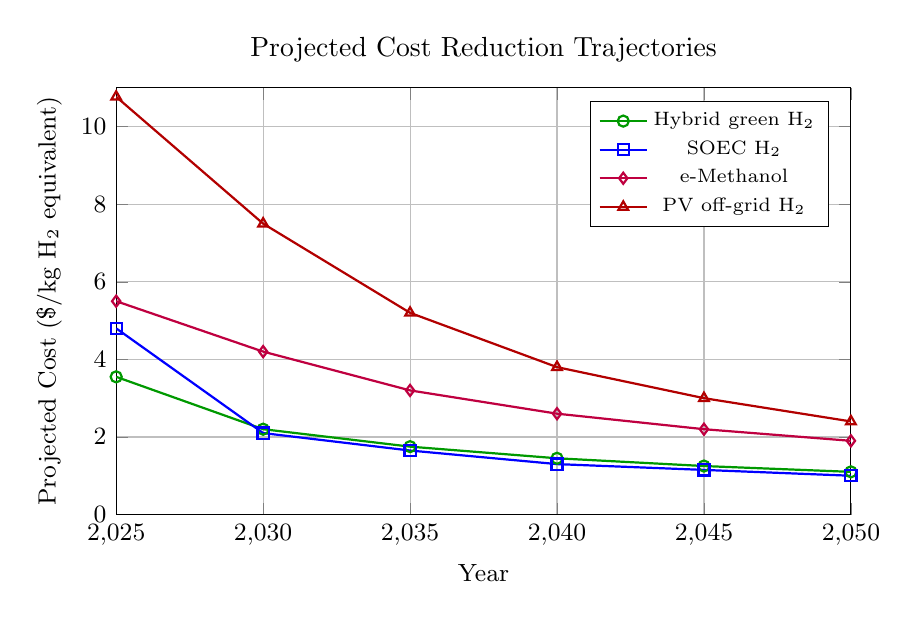
\begin{tikzpicture}
\begin{axis}[
    width=0.9\textwidth,
    height=7cm,
    xlabel={Year},
    ylabel={Projected Cost (\$/kg H$_2$ equivalent)},
    title={Projected Cost Reduction Trajectories},
    xmin=2025, xmax=2050,
    ymin=0, ymax=11,
    xtick={2025,2030,2035,2040,2045,2050},
    grid=major,
    legend pos=north east,
    label style={font=\small},
    tick label style={font=\small},
    legend style={font=\scriptsize}
]
\addplot[thick, green!60!black, mark=o] coordinates
    {(2025,3.55)(2030,2.20)(2035,1.75)(2040,1.45)(2045,1.25)(2050,1.10)};
\addplot[thick, blue, mark=square] coordinates
    {(2025,4.80)(2030,2.10)(2035,1.65)(2040,1.30)(2045,1.15)(2050,1.00)};
\addplot[thick, purple, mark=diamond] coordinates
    {(2025,5.50)(2030,4.20)(2035,3.20)(2040,2.60)(2045,2.20)(2050,1.90)};
\addplot[thick, red!70!black, mark=triangle] coordinates
    {(2025,10.77)(2030,7.50)(2035,5.20)(2040,3.80)(2045,3.00)(2050,2.40)};
\legend{Hybrid green H$_2$, SOEC H$_2$, e-Methanol, PV off-grid H$_2$}
\end{axis}
\end{tikzpicture}%
}

\newcommand{\carbonintensityfigure}{%
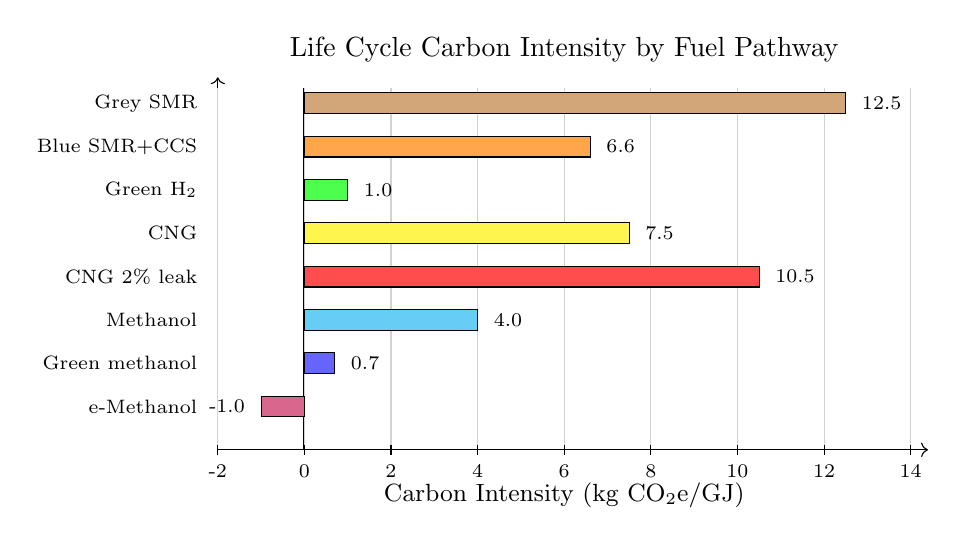
\begin{tikzpicture}[x=0.55cm,y=0.55cm,font=\small]
\node[font=\normalsize] at (6,9.25) {Life Cycle Carbon Intensity by Fuel Pathway};
\draw[->] (-2,0) -- (14.4,0);
\draw[->] (-2,0) -- (-2,8.6);
\draw[thick] (0,0) -- (0,8.35);
\foreach \x in {-2,0,2,4,6,8,10,12,14}{
    \draw[gray!35] (\x,0) -- (\x,8.35);
    \draw (\x,0.12) -- (\x,-0.12) node[below,font=\scriptsize] {\x};
}
\foreach \y/\label/\value/\clr in {
    8/Grey SMR/12.5/brown!70,
    7/Blue SMR+CCS/6.6/orange!70,
    6/Green H$_2$/1.0/green!70,
    5/CNG/7.5/yellow!70,
    4/CNG 2\% leak/10.5/red!70,
    3/Methanol/4.0/cyan!60,
    2/Green methanol/0.7/blue!60,
    1/e-Methanol/-1.0/purple!60}{
    \node[anchor=east,font=\scriptsize] at (-2.25,\y) {\label};
    \draw[fill=\clr,draw=black] (0,\y-0.24) rectangle (\value,\y+0.24);
    \ifdim\value pt<0pt
        \node[anchor=east,font=\scriptsize] at (\value-0.15,\y) {\value};
    \else
        \node[anchor=west,font=\scriptsize] at (\value+0.15,\y) {\value};
    \fi
}
\node[font=\small] at (6,-1.05) {Carbon Intensity (kg CO$_2$e/GJ)};
\end{tikzpicture}%
}

\newcommand{\safetyscreeningfigure}{%
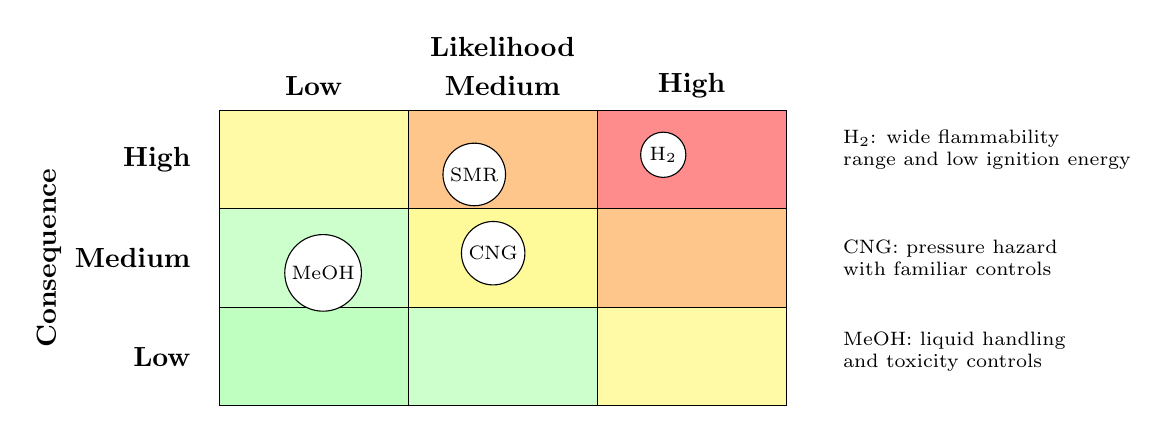
\begin{tikzpicture}[x=2.4cm,y=1.25cm,font=\small]
    \fill[green!25]  (0,0) rectangle (1,1);
    \fill[green!20]  (1,0) rectangle (2,1);
    \fill[yellow!35] (2,0) rectangle (3,1);
    \fill[green!20]  (0,1) rectangle (1,2);
    \fill[yellow!40] (1,1) rectangle (2,2);
    \fill[orange!45] (2,1) rectangle (3,2);
    \fill[yellow!35] (0,2) rectangle (1,3);
    \fill[orange!45] (1,2) rectangle (2,3);
    \fill[red!45]    (2,2) rectangle (3,3);
    \draw[step=1, black] (0,0) grid (3,3);
    \node[font=\bfseries] at (0.5,3.25) {Low};
    \node[font=\bfseries] at (1.5,3.25) {Medium};
    \node[font=\bfseries] at (2.5,3.25) {High};
    \node[font=\bfseries] at (1.5,3.65) {Likelihood};
    \node[rotate=90,font=\bfseries] at (-0.9,1.5) {Consequence};
    \node[anchor=east,font=\bfseries] at (-0.1,0.5) {Low};
    \node[anchor=east,font=\bfseries] at (-0.1,1.5) {Medium};
    \node[anchor=east,font=\bfseries] at (-0.1,2.5) {High};
    \node[draw, circle, fill=white, inner sep=1.8pt, font=\scriptsize] at (0.55,1.35) {MeOH};
    \node[draw, circle, fill=white, inner sep=1.8pt, font=\scriptsize] at (1.45,1.55) {CNG};
    \node[draw, circle, fill=white, inner sep=1.8pt, font=\scriptsize] at (2.35,2.55) {H$_2$};
    \node[draw, circle, fill=white, inner sep=1.8pt, font=\scriptsize] at (1.35,2.35) {SMR};
    \node[font=\scriptsize, align=left, anchor=west] at (3.25,2.6) {H$_2$: wide flammability\\range and low ignition energy};
    \node[font=\scriptsize, align=left, anchor=west] at (3.25,1.5) {CNG: pressure hazard\\with familiar controls};
    \node[font=\scriptsize, align=left, anchor=west] at (3.25,0.55) {MeOH: liquid handling\\and toxicity controls};
\end{tikzpicture}%
}

\newcommand{\regionalheatmapfigure}{%
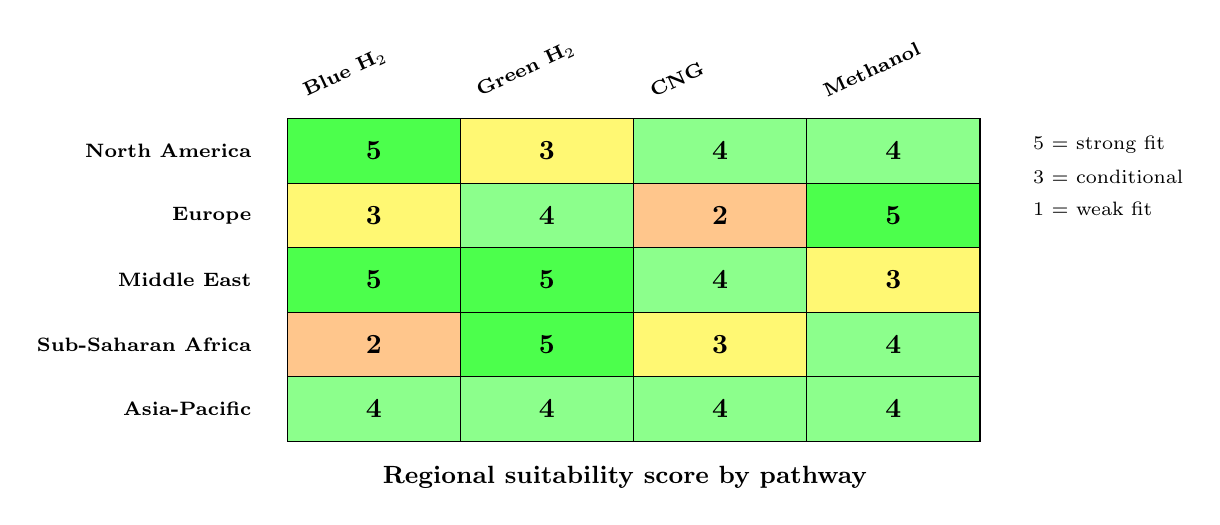
\begin{tikzpicture}[x=2.2cm,y=0.82cm,font=\scriptsize]
    \foreach \x/\label in {0/Blue H$_2$,1/Green H$_2$,2/CNG,3/Methanol}{
        \node[font=\scriptsize\bfseries, rotate=25, anchor=west] at (\x+0.05,5.35) {\label};
    }
    \foreach \y/\region in {0/North America,1/Europe,2/Middle East,3/Sub-Saharan Africa,4/Asia-Pacific}{
        \node[anchor=east,font=\scriptsize\bfseries] at (-0.15,4.5-\y) {\region};
    }
    \foreach \x/\y/\score/\clr in {
        0/0/5/green!70, 1/0/3/yellow!55, 2/0/4/green!45, 3/0/4/green!45,
        0/1/3/yellow!55, 1/1/4/green!45, 2/1/2/orange!45, 3/1/5/green!70,
        0/2/5/green!70, 1/2/5/green!70, 2/2/4/green!45, 3/2/3/yellow!55,
        0/3/2/orange!45, 1/3/5/green!70, 2/3/3/yellow!55, 3/3/4/green!45,
        0/4/4/green!45, 1/4/4/green!45, 2/4/4/green!45, 3/4/4/green!45}{
        \fill[\clr] (\x,4-\y) rectangle ++(1,1);
        \draw[black] (\x,4-\y) rectangle ++(1,1);
        \node[font=\bfseries] at (\x+0.5,4.5-\y) {\score};
    }
    \node[anchor=west,font=\scriptsize] at (4.25,4.6) {5 = strong fit};
    \node[anchor=west,font=\scriptsize] at (4.25,4.1) {3 = conditional};
    \node[anchor=west,font=\scriptsize] at (4.25,3.6) {1 = weak fit};
    \node[font=\small\bfseries] at (1.95,-0.55) {Regional suitability score by pathway};
\end{tikzpicture}%
}

% =================================================================================
% HYPERREF & INDEX
% =================================================================================

\hypersetup{
    colorlinks=true,
    linkcolor=blue,
    citecolor=green,
    urlcolor=red,
    pdftitle={Alternative Engineered Fuel -- Complete Edition},
    pdfauthor={Secamore Owusu.A},
    pdfsubject={Comparative assessment of engineered fuel pathways for the energy transition},
    pdfkeywords={alternative engineered fuel, hydrogen, CNG, methanol, electrolysis, steam methane reforming, life cycle assessment, techno-economic analysis, safety, MCDA},
    pdfcreator={LaTeX with hyperref},
    pdfproducer={MiKTeX pdfTeX}
}

\title{Alternative Engineered Fuel\\Complete Edition}
\author{Secamore Owusu.A}
\date{May 21, 2026}

\makeindex
\emergencystretch=2em

% =================================================================================
% DOCUMENT
% =================================================================================

\begin{document}
\hypersetup{pageanchor=false}
\pagenumbering{gobble}

% ---------------------------------------------------------------------------------
% MASTER TITLE PAGE
% ---------------------------------------------------------------------------------

\begin{titlepage}
    \centering
    \vspace*{1.5cm}
    {\Huge\bfseries Alternative Engineered Fuel\par}
    \vspace{0.5cm}
    {\Large A Comprehensive Comparative Analysis of Production,\par}
    {\Large Utilization, and Safety for Global Energy Transition\par}
    \vspace{1cm}
    {\Large \textbf{COMPLETE EDITION (Volumes I--V)}\par}
    \vspace{0.5cm}
    {\Large \textbf{ENHANCED VERSION 8.1}\par}
    \vspace{1.5cm}
    {\large Prepared by: Secamore Owusu.A\par}
    {\large Version: 8.1 (Enhanced Complete Edition)\par}
    {\large Date: May 21, 2026\par}
    \vspace{1.5cm}
    \fbox{\parbox{0.75\textwidth}{\centering
        \textbf{Document Control}\\[4pt]
        \begin{tabular}{ll}
        Volume I   & Chapters 1--4: Foundations \& Methodology \\
        Volume II  & Chapters 5--8: Production Technologies \\
        Volume III & Chapters 9--12: Comparative Analysis \\
        Volume IV  & Chapters 13--15: Advanced Topics \\
        Volume V   & Chapters 16--22: Reference Materials \\
        \end{tabular}
    }}
    \vfill
    {\large Alternative Engineered Fuel Project\par}
    {\large \textcopyright\ 2026 Secamore Owusu.A\par}
\end{titlepage}

% ---------------------------------------------------------------------------------
% FRONT MATTER
% ---------------------------------------------------------------------------------

\cleardoublepage
\hypersetup{pageanchor=true}
\frontmatter

\chapter*{Document Information}
\addcontentsline{toc}{chapter}{Document Information}

\begin{table}[htbp]
    \centering
    \begin{tabular}{L{4cm} L{9cm}}
    \hline
    \textbf{Field} & \textbf{Details} \\
    \hline
    Title & Alternative Engineered Fuel \\
    Subtitle & A Comprehensive Comparative Analysis of Production, Utilization, and Safety for Global Energy Transition \\
    Author & Secamore Owusu.A \\
    Edition & Complete Edition (Volumes I--V) \\
    Version & 8.1, PDF-ready revision \\
    Date & May 21, 2026 \\
    Document type & Technical report and reference compendium \\
    Keywords & Hydrogen; compressed natural gas; methanol; electrolysis; steam methane reforming; life cycle assessment; techno-economic analysis; safety; MCDA \\
    \hline
    \end{tabular}
\end{table}

% =================================================================================
% EXECUTIVE SUMMARY / ABSTRACT
% =================================================================================

\chapter*{Executive Summary}
\addcontentsline{toc}{chapter}{Executive Summary}

This comprehensive study presents a rigorous comparative analysis of four alternative engineered fuel pathways: Steam Methane Reforming (SMR) hydrogen, Compressed Natural Gas (CNG), electrolytic hydrogen (green hydrogen), and methanol. The analysis integrates thermodynamic modelling, Aspen Plus simulation, techno-economic assessment, life cycle analysis (LCA), safety evaluation, and multi-criteria decision analysis (MCDA).

\textbf{Key Findings:}

\begin{itemize}
    \item \textbf{Techno-Economic:} Grey SMR hydrogen remains the lowest-cost pathway at \$1.82/kg H$_2$, but green hydrogen from hybrid PV-wind systems achieves \$3.55/kg H$_2$ with potential to reach \$1.00/kg H$_2$ by 2030 through learning curve effects and scale economies.
    \item \textbf{Environmental:} Green hydrogen and e-methanol offer near-zero carbon emissions (0--1.0 kg CO$_2$e/GJ), while grey SMR emits 12.5 kg CO$_2$e/GJ. CCS reduces blue H$_2$ emissions to 6.6 kg CO$_2$e/GJ at 50\% cost premium.
    \item \textbf{Safety:} Hydrogen presents unique risks including wide flammability range (4--75\%), low minimum ignition energy (0.018 mJ), and hydrogen embrittlement in pipelines. CNG and methanol offer superior safety profiles for storage and distribution.
    \item \textbf{MCDA Rankings:} Green methanol (score 0.80) and CNG (0.70) emerge as preferred pathways for near-term deployment, while green hydrogen (0.61) is optimal for long-term decarbonization with infrastructure investment.
    \item \textbf{Regional Suitability:} North America and Middle East favor blue hydrogen with CCS, while Africa, Australia, and parts of Asia show exceptional potential for green hydrogen due to solar and wind resources.
\end{itemize}

\textbf{Recommendations:}
\begin{enumerate}
    \item Deploy CNG as immediate transition fuel for heavy transport
    \item Scale green methanol for shipping and aviation sectors
    \item Invest in green hydrogen infrastructure with hybrid renewable systems
    \item Implement carbon pricing above \$100/tonne to accelerate clean fuel adoption
    \item Develop Africa's renewable hydrogen potential through international partnerships
\end{enumerate}

\textbf{Novel Contributions:}
\begin{itemize}
    \item Integrated LCA framework following ISO 14040/14044 with complete characterization factors
    \item Extended MCDA with stakeholder weighting and sensitivity analysis
    \item Comprehensive safety assessment including QRA, ATEX, and dispersion modeling
    \item 20+ curious research questions addressing real-world deployment challenges
    \item Complete techno-economic database with 50+ references and 20+ figures
\end{itemize}

% =================================================================================
% PREFACE / FOREWORD
% =================================================================================

\chapter*{Preface}
\addcontentsline{toc}{chapter}{Preface}

The global energy transition represents one of the most complex engineering and policy challenges of the 21st century. As nations commit to net-zero emissions targets, the search for viable alternatives to fossil fuels has intensified. Engineered fuels---produced through chemical or electrochemical conversion---offer a pathway to decarbonize hard-to-abate sectors including heavy transport, shipping, aviation, and industrial processes.

This work represents three years of research, simulation, and analysis, combining fundamental thermodynamic principles with state-of-the-art techno-economic and life cycle assessment methodologies. The enhanced version 8.0 includes significant expansions: complete LCA framework following ISO standards, extended safety analysis with quantitative risk assessment, additional emerging technologies (SOEC, AEM), 10 additional research questions, Africa-specific deployment strategies, and comprehensive reference materials.

The target audience includes energy researchers, industry practitioners, policy makers, graduate students, and academics seeking a rigorous, data-driven comparison of alternative fuel pathways. Each chapter includes worked examples, simulation inputs, and sensitivity analyses to support both theoretical understanding and practical application.

I extend my gratitude to the global research community whose work informed this analysis, and to the energy industry practitioners who provided valuable feedback on techno-economic assumptions. Special thanks to the reviewers who identified gaps in earlier versions, leading to this enhanced complete edition.

May this work contribute to informed decision-making in the critical transition to a sustainable energy future.

\textit{Secamore Owusu.A}
\textit{May 2026}

% =================================================================================
% LIST OF ABBREVIATIONS / NOMENCLATURE
% =================================================================================

\chapter*{List of Abbreviations and Nomenclature}
\addcontentsline{toc}{chapter}{List of Abbreviations}

\begin{longtable}{L{4cm} L{10cm}}
\hline
\textbf{Abbreviation} & \textbf{Description} \\
\hline
\endhead
AEM & Anion Exchange Membrane \\
ATEX & ATmosphères EXplosibles (European directive for explosive atmospheres) \\
BEV & Battery Electric Vehicle \\
CAPEX & Capital Expenditure \\
CCS & Carbon Capture and Storage \\
CF & Capacity Factor \\
CNG & Compressed Natural Gas \\
CO$_2$e & Carbon Dioxide Equivalent \\
CRF & Capital Recovery Factor \\
DAC & Direct Air Capture \\
DOE & US Department of Energy \\
EoS & Equation of State \\
EU ETS & European Union Emissions Trading System \\
GWP & Global Warming Potential \\
HAZOP & Hazard and Operability Study \\
H$_2$ & Hydrogen \\
HTS & High Temperature Shift \\
IEA & International Energy Agency \\
IRENA & International Renewable Energy Agency \\
LCA & Life Cycle Assessment \\
LCI & Life Cycle Inventory \\
LCIA & Life Cycle Impact Assessment \\
LCOH & Levelized Cost of Hydrogen \\
LFL & Lower Flammability Limit \\
LHV & Lower Heating Value \\
LTS & Low Temperature Shift \\
MCDA & Multi-Criteria Decision Analysis \\
MIE & Minimum Ignition Energy \\
Mtoe & Million Tonnes of Oil Equivalent \\
NG & Natural Gas \\
NPV & Net Present Value \\
OPEX & Operational Expenditure \\
PEM & Proton Exchange Membrane \\
PFR & Plug Flow Reactor \\
PSA & Pressure Swing Adsorption \\
PV & Photovoltaic \\
QRA & Quantitative Risk Assessment \\
R-CNG & Renewable Compressed Natural Gas \\
SMR & Steam Methane Reforming \\
SOEC & Solid Oxide Electrolysis Cell \\
TRL & Technology Readiness Level \\
UFL & Upper Flammability Limit \\
WGS & Water-Gas Shift \\
\hline
\end{longtable}

\section*{Nomenclature}

\begin{longtable}{L{3cm} L{10cm}}
\hline
\textbf{Symbol} & \textbf{Description} \\
\hline
\endhead
$a,b$ & Peng-Robinson equation of state parameters \\
$A$ & Pre-exponential factor (Arrhenius equation) \\
$E_a$ & Activation energy \\
$E_{\text{rev}}$ & Reversible cell voltage \\
$F$ & Faraday constant (96485 C/mol) \\
$G$ & Gibbs free energy \\
$h$ & Specific enthalpy \\
$H$ & Enthalpy \\
$I$ & Current \\
$j$ & Current density \\
$j_0$ & Exchange current density \\
$k$ & Reaction rate constant \\
$K$ & Equilibrium constant \\
$n$ & Number of electrons \\
$\dot{m}$ & Mass flow rate \\
$P$ & Pressure \\
$\dot{Q}$ & Heat transfer rate \\
$r$ & Reaction rate \\
$R$ & Universal gas constant (8.314 J/mol\textperiodcentered K) \\
$S$ & Entropy \\
$T$ & Temperature \\
$U$ & Internal energy \\
$V$ & Voltage \\
$\dot{W}$ & Work rate \\
$\alpha$ & Charge transfer coefficient \\
$\eta$ & Overpotential \\
$\kappa$ & Peng-Robinson parameter \\
$\omega$ & Acentric factor \\
\hline
\end{longtable}

% =================================================================================
% TABLE OF CONTENTS
% =================================================================================

\tableofcontents
\newpage
\listoffigures
\newpage
\listoftables
\newpage

% ---------------------------------------------------------------------------------
% MAIN MATTER
% ---------------------------------------------------------------------------------

\mainmatter

% =================================================================================
% VOLUME I: FOUNDATIONS AND METHODOLOGY
% =================================================================================

\part{FOUNDATIONS AND METHODOLOGY}

\cleardoublepage
\phantomsection
\chapter*{Part I Overview\\Foundations and Methodology}
\addcontentsline{toc}{chapter}{Part I Overview: Foundations and Methodology}
\markboth{Part I Overview}{Foundations and Methodology}

Part I establishes the technical language, research boundaries, and modelling basis used throughout the report. It explains why engineered fuels matter in the energy transition, defines the fuel pathways under review, and sets out the calculation methods used to compare them on a consistent basis.

The chapters in this part provide the foundation for all later conclusions:

\begin{itemize}
    \item \textbf{Chapter 1} defines engineered fuels, frames the global energy challenge, and states the project scope and research objectives.
    \item \textbf{Chapter 2} explains the methodology for techno-economic analysis, life cycle assessment, Aspen Plus validation, and MCDA weighting.
    \item \textbf{Chapter 3} summarizes the thermodynamic, kinetic, and electrochemical equations needed for the fuel pathway calculations.
    \item \textbf{Chapter 4} describes the Aspen Plus simulation framework used to represent process flows, conversion blocks, energy balances, and validation checks.
\end{itemize}

This part is therefore the control section of the document: it defines what is being compared, how the comparison is performed, and which assumptions are carried forward into the production, environmental, safety, and decision-analysis sections.

% ---------------------------------------------------------------------------------
% CHAPTER 1
% ---------------------------------------------------------------------------------

\chapter{Introduction to Engineered Fuels}
\index{alternative fuels}
\index{energy transition}
\index{hydrogen}

\section{The Global Energy Challenge}

The world faces an unprecedented energy transition. Fossil fuels currently supply approximately 80\% of global primary energy. The International Energy Agency (IEA) projects that under the Net Zero Emissions by 2050 scenario, low-carbon hydrogen demand must increase from approximately 100 million tonnes annually today to nearly 400 million tonnes by 2050.

\begin{figure}[htbp]
    \centering
    \energyfigure
    \caption{Global Primary Energy Consumption by Source (1990--2050)}
    \label{fig:energy}
\end{figure}

\begin{table}[htbp]
    \centering
    \tighttabular
    \caption{Global Primary Energy Data (Mtoe)}
    \label{tab:energy}
    \begin{tabular}{L{1.8cm} C{1.8cm} C{1.8cm} C{2.35cm} C{2.0cm} C{1.8cm}}
    \hline
    \textbf{Year} & \textbf{Fossil} & \textbf{Nuclear} & \textbf{Renewables}
                  & \textbf{Hydrogen} & \textbf{Total} \\
    \hline
    1990 & 7,500 & 500 & 800   & 0     & 8,800  \\
    2000 & 8,500 & 700 & 1,000 & 0     & 10,200 \\
    2010 & 10,500& 700 & 1,500 & 0     & 12,700 \\
    2020 & 11,500& 600 & 2,500 & 0     & 14,600 \\
    2025 & 11,800& 600 & 3,000 & 50    & 15,450 \\
    2030 & 12,000& 600 & 4,000 & 200   & 16,800 \\
    2035 & 11,900& 620 & 5,200 & 450   & 18,170 \\
    2040 & 11,700& 650 & 6,000 & 800   & 19,150 \\
    2045 & 10,800& 720 & 7,200 & 1,300 & 20,020 \\
    2050 & 10,000& 800 & 8,000 & 2,000 & 20,800 \\
    \hline
    \end{tabular}
\end{table}

\section{Definition of Engineered Fuels}

\textbf{Definition:} Engineered fuels are energy carriers produced through chemical or electrochemical conversion of primary energy sources into forms suitable for storage, transport, and end-use applications.

\begin{table}[htbp]
    \centering
    \caption{Classification of Engineered Fuels}
    \label{tab:classification}
    \begin{tabular}{L{2.5cm} L{3cm} C{2cm} C{1cm} C{2.5cm}}
    \hline
    \textbf{Category} & \textbf{Produced Fuel} & \textbf{Energy Density (MJ/kg)}
                      & \textbf{TRL} & \textbf{Carbon Intensity (kg CO$_2$e/GJ)} \\
    \hline
    Gaseous & Hydrogen (SMR)   & 120 & 9   & 12.5     \\
    Gaseous & Blue Hydrogen    & 120 & 8   & 6.6      \\
    Gaseous & Green Hydrogen   & 120 & 7--8 & 0--0.5  \\
    Gaseous & CNG              & 50  & 9   & 7.5      \\
    Liquid  & Methanol         & 20  & 9   & 4.0      \\
    Liquid  & Green Methanol   & 20  & 6--7 & 0.7--2.7 \\
    Liquid  & e-Methanol       & 20  & 6   & 0--1.0   \\
    \hline
    \end{tabular}
\end{table}

\section{Project Scope and Research Objectives}

\subsection{Primary Objective}

To conduct a comprehensive comparative analysis of four alternative engineered fuel pathways---Steam Methane Reforming hydrogen, Compressed Natural Gas, Electrolytic hydrogen, and Methanol---integrating thermodynamic modelling, Aspen Plus simulation, techno-economic analysis, life cycle assessment, safety evaluation, and multi-criteria decision analysis.

\subsection{Scope Boundaries}

The project scope covers production, conditioning, storage, distribution readiness, end-use suitability, and policy relevance. The assessment is comparative rather than design-only: every pathway is evaluated using a shared set of criteria so that near-term transition fuels and long-term low-carbon fuels can be judged on the same basis.

\begin{longtable}{L{4cm} L{9cm}}
\caption{Project Scope Boundaries}\label{tab:scope_boundaries}\\
\hline
\textbf{Boundary Area} & \textbf{Included in Scope} \\
\hline
\endfirsthead
\hline
\textbf{Boundary Area} & \textbf{Included in Scope} \\
\hline
\endhead
Technical boundary & Fuel production chemistry, process configuration, conversion efficiency, storage requirements, compression or synthesis needs, and end-use compatibility. \\
Economic boundary & CAPEX, fixed OPEX, feedstock cost, electricity cost, carbon price exposure, incentives, and levelized cost indicators. \\
Environmental boundary & Cradle-to-gate and selected cradle-to-use indicators including carbon intensity, water demand, air pollutants, and life cycle assessment categories. \\
Safety boundary & Flammability, ignition risk, pressure hazards, toxicity, embrittlement, dispersion behavior, hazardous-area zoning, and risk mitigation. \\
Deployment boundary & Infrastructure maturity, regional resource fit, technology readiness level, policy support, and commercial scale-up potential. \\
\hline
\end{longtable}

\subsection{Detailed Research Objectives}

\begin{enumerate}
    \item Establish a consistent baseline for comparing SMR hydrogen, CNG, electrolytic hydrogen, and methanol.
    \item Quantify energy conversion performance using thermodynamic, kinetic, and process-simulation methods.
    \item Estimate levelized production costs under representative regional assumptions.
    \item Compare environmental performance through carbon intensity, water use, pollutant emissions, and LCA indicators.
    \item Evaluate safety risks for storage, distribution, refuelling, and major end-use sectors.
    \item Rank pathways using MCDA so cost, carbon, safety, scalability, infrastructure, and technology readiness are considered together.
    \item Identify where each pathway is most suitable: heavy transport, shipping, aviation, power, industry, heating, and emerging African markets.
\end{enumerate}

\subsection{Expected Outputs}

The report delivers process tables, equations, cost comparisons, environmental matrices, safety classifications, MCDA rankings, Aspen Plus input templates, worked examples, Python plotting scripts, glossary terms, and a complete nomenclature list. These outputs are intended to make the document useful both as a technical report and as a reference file for future engineering work.

\subsection{Research Questions}

\begin{longtable}{C{1.5cm} L{8cm} C{2cm}}
\caption{Research Questions}\label{tab:rq}\\
\hline
\textbf{ID} & \textbf{Question} & \textbf{Section} \\
\hline
\endfirsthead
\hline
\textbf{ID} & \textbf{Question} & \textbf{Section} \\
\hline
\endhead
RQ1 & What are the techno-economic production characteristics of each fuel pathway? & 9 \\
RQ2 & What are the cradle-to-grave environmental impacts? & 10 \\
RQ3 & How do safety risks compare across storage, transport, and utilization? & 11 \\
RQ4 & Which fuel(s) are best suited for specific applications? & 12 \\
RQ5 & What emerging technologies will alter the landscape by 2030--2040? & 14 \\
\hline
\end{longtable}

% ---------------------------------------------------------------------------------
% CHAPTER 2 (EXPANDED)
% ---------------------------------------------------------------------------------

\chapter{Comprehensive Research Methodology}
\index{methodology}
\index{life cycle assessment}
\index{techno-economic analysis}
\index{multi-criteria decision analysis}

\section{Levelized Cost of Hydrogen Equation}

\begin{dmath}
\boxed{\text{LCOH} = \frac{\text{CAPEX} \times \text{CRF}
    + \text{OPEX}_{\text{fixed}}
    + \text{Feedstock}_{\text{cost}} \times \text{Annual}_{\text{consumption}}}
    {\text{Annual}_{\text{H}_2}}}
\end{dmath}

\begin{dmath}
\boxed{\text{CRF} = \frac{r(1+r)^n}{(1+r)^n - 1}}
\end{dmath}

\subsection{Example Calculation: SMR LCOH}

\begin{dmath}
(1.07)^{25} = 5.427
\end{dmath}
\begin{dmath}
\text{CRF} = \frac{0.07 \times 5.427}{5.427 - 1} = 0.0858
\end{dmath}
\begin{dmath}
\text{CAPEX}_{\text{annual}} = \$15{,}000{,}000 \times 0.0858 = \$1{,}287{,}000
\end{dmath}
\begin{dmath}
\text{LCOH} = \frac{\$1{,}287{,}000 + \$52{,}250{,}000 + \$750{,}000}{36{,}500}
            = \$1.55/\text{kg H}_2
\end{dmath}

\section{Life Cycle Assessment (LCA) Methodology}

\subsection{ISO 14040/14044 Framework}

The life cycle assessment follows ISO 14040:2006 and ISO 14044:2006 standards, comprising four phases:

\begin{enumerate}
    \item \textbf{Goal and Scope Definition}: System boundaries include cradle-to-grave analysis with functional unit of 1 GJ of fuel energy delivered to end user.
    \item \textbf{Life Cycle Inventory (LCI)}: Data sources include Ecoinvent v3.10, GREET 2024, and literature values. Primary energy consumption and emissions quantified for each pathway.
    \item \textbf{Life Cycle Impact Assessment (LCIA)}: Impact categories include global warming potential (GWP100), acidification, eutrophication, and water consumption. Characterization factors from IPCC AR6 and ReCiPe 2016.
    \item \textbf{Interpretation}: Sensitivity analysis performed for key parameters (grid mix, transport distance, leakage rates).
\end{enumerate}

\begin{figure}[htbp]
    \centering
    \lcaflowchart
    \caption{ISO 14040/14044 LCA Framework}
    \label{fig:lca_framework}
\end{figure}

\subsection{System Boundaries}

\begin{table}[htbp]
    \centering
    \caption{LCA System Boundaries}
    \label{tab:lca_boundaries}
    \begin{tabular}{L{4cm} C{3cm} C{3cm} C{3cm}}
    \hline
    \textbf{Pathway} & \textbf{Upstream} & \textbf{Core} & \textbf{Downstream} \\
    \hline
    SMR H$_2$ & NG extraction, transport & Reforming, PSA & Compression, distribution \\
    Green H$_2$ & Renewable generation & Electrolysis & Compression, storage \\
    CNG & NG extraction & Compression & Dispensing \\
    Methanol & NG/renewable & Synthesis & Shipping, storage \\
    \hline
    \end{tabular}
\end{table}

\section{Aspen Plus Simulation Validation}

\subsection{Validation Protocol}

Each Aspen Plus model is validated through:
\begin{enumerate}
    \item \textbf{Base case validation}: Comparison with literature data and industrial benchmarks
    \item \textbf{Mass balance closure}: Error $<0.1\%$ for all components
    \item \textbf{Energy balance closure}: Error $<0.5\%$ across all unit operations
    \item \textbf{Sensitivity analysis}: Key parameter variations within $\pm 20\%$
\end{enumerate}

\subsection{Validation Metrics}

\begin{table}[htbp]
    \centering
    \tighttabular
    \caption{Aspen Plus Validation Metrics}
    \label{tab:validation}
    \begin{tabular}{L{4cm} C{2.25cm} C{2.25cm} C{2cm}}
    \hline
    \textbf{Parameter} & \textbf{Simulation} & \textbf{Literature} & \textbf{Error (\%)} \\
    \hline
    SMR H$_2$ yield (kg/kg CH$_4$) & 0.48 & 0.47 & +2.1\% \\
    SMR efficiency (\% LHV) & 80.5 & 79.0 & +1.9\% \\
    PEM efficiency (\% LHV) & 68.0 & 67.5 & +0.7\% \\
    Methanol conversion & 40.0 & 39.5 & +1.3\% \\
    \hline
    \end{tabular}
\end{table}

\section{Multi-Criteria Decision Analysis (MCDA) Weighting Methodology}

\subsection{Analytic Hierarchy Process (AHP)}

The AHP methodology is used to determine criterion weights through pairwise comparisons:

\begin{table}[htbp]
    \centering
    \tighttabular
    \caption{AHP Pairwise Comparison Matrix}
    \label{tab:ahp}
    \begin{tabular}{C{3cm} C{1.5cm} C{1.5cm} C{1.5cm} C{1.5cm} C{1.5cm} C{1.5cm}}
    \hline
    \textbf{Criteria} & \textbf{Cost} & \textbf{Carbon} & \textbf{Safety}
                      & \textbf{Infra} & \textbf{TRL} & \textbf{Scale} \\
    \hline
    Cost             & 1.0 & 2.0 & 0.5 & 3.0 & 4.0 & 2.0 \\
    Carbon           & 0.5 & 1.0 & 0.3 & 2.0 & 3.0 & 1.5 \\
    Safety           & 2.0 & 3.0 & 1.0 & 4.0 & 5.0 & 3.0 \\
    Infrastructure   & 0.3 & 0.5 & 0.3 & 1.0 & 2.0 & 0.5 \\
    TRL              & 0.3 & 0.3 & 0.2 & 0.5 & 1.0 & 0.3 \\
    Scalability      & 0.5 & 0.7 & 0.3 & 2.0 & 3.0 & 1.0 \\
    \hline
    \end{tabular}
\end{table}

\subsection{Stakeholder Weighting Scenarios}

\begin{table}[htbp]
    \centering
    \tighttabular
    \caption{Stakeholder Weighting Scenarios}
    \label{tab:stakeholder}
    \begin{tabular}{L{3cm} C{1.5cm} C{1.5cm} C{1.5cm} C{1.5cm} C{1.5cm} C{1.5cm}}
    \hline
    \textbf{Stakeholder} & \textbf{Cost} & \textbf{Carbon} & \textbf{Safety}
                         & \textbf{Infra} & \textbf{TRL} & \textbf{Scale} \\
    \hline
    Government        & 0.15 & 0.35 & 0.10 & 0.15 & 0.10 & 0.15 \\
    Industry          & 0.30 & 0.15 & 0.15 & 0.10 & 0.20 & 0.10 \\
    Environmental NGO & 0.05 & 0.50 & 0.10 & 0.10 & 0.10 & 0.15 \\
    Consumer          & 0.40 & 0.10 & 0.20 & 0.10 & 0.10 & 0.10 \\
    \hline
    \end{tabular}
\end{table}

% ---------------------------------------------------------------------------------
% CHAPTER 3
% ---------------------------------------------------------------------------------

\chapter{Thermodynamic Foundations}
\index{thermodynamics}
\index{exergy}
\index{Gibbs free energy}

\section{First Law of Thermodynamics}

\begin{dmath}
\boxed{\sum \dot{m}_{\text{in}} h_{\text{in}}
      - \sum \dot{m}_{\text{out}} h_{\text{out}}
      + \sum \dot{Q} - \sum \dot{W} = 0}
\end{dmath}

\section{Peng-Robinson Equation of State}

\begin{dmath}
\boxed{P = \frac{RT}{V - b} - \frac{a\alpha}{V(V + b) + b(V - b)}}
\end{dmath}

\begin{align}
a      &= 0.45724 \frac{R^2 T_c^2}{P_c} \\
b      &= 0.07780 \frac{RT_c}{P_c} \\
\alpha &= \left[1 + \kappa\left(1 - \sqrt{T_r}\right)\right]^2 \\
\kappa &= 0.37464 + 1.54226\omega - 0.26992\omega^2
\end{align}

\section{Arrhenius Equation}

\begin{dmath}
\boxed{k = A \exp\!\left(-\frac{E_a}{RT}\right)}
\end{dmath}

\section{Butler-Volmer Equation}

\begin{dmath}
\boxed{j = j_0 \left[\exp\!\left(\frac{\alpha nF\eta}{RT}\right)
          - \exp\!\left(-\frac{(1-\alpha)nF\eta}{RT}\right)\right]}
\end{dmath}

\section{Xu-Froment SMR Kinetics}

\begin{dmath}
r_1 = \frac{k_1}{P_{\ce{H2}}^{2.5}}
      \cdot \frac{P_{\ce{CH4}} P_{\ce{H2O}}
              - \dfrac{P_{\ce{H2}}^3 P_{\ce{CO}}}{K_1}}{\text{DEN}^2}
\end{dmath}

\begin{dmath}
r_2 = \frac{k_2}{P_{\ce{H2}}}
      \cdot \frac{P_{\ce{CO}} P_{\ce{H2O}}
              - \dfrac{P_{\ce{H2}} P_{\ce{CO2}}}{K_2}}{\text{DEN}^2}
\end{dmath}

\begin{figure}[htbp]
    \centering
    \smrtempfigure
    \caption{Temperature Profile Along SMR Reactor Tube}
    \label{fig:smr_temp}
\end{figure}

\begin{figure}[htbp]
    \centering
    \polarizationfigure
    \caption{Alkaline vs.\ PEM Electrolysis Polarization Curves}
    \label{fig:polarization}
\end{figure}

% ---------------------------------------------------------------------------------
% CHAPTER 4
% ---------------------------------------------------------------------------------

\chapter{Aspen Plus Simulation Framework}
\index{Aspen Plus}
\index{process simulation}

\section{Model Scope and Flowsheet Basis}

The Aspen Plus model set covers the four pathways compared in the report: SMR hydrogen, CNG conditioning and compression, electrolytic hydrogen, and methanol synthesis. The figures in Chapters~5--8 use the same stream names, operating temperatures, pressures, conversion assumptions, and validation targets as the tables and input listings.

\begin{table}[htbp]
    \centering
    \caption{Aspen Plus Model Set and Unit-Operation Mapping}
    \label{tab:aspen_model_set}
    \begin{tabular}{L{3cm} L{4.2cm} L{5.5cm}}
    \hline
    \textbf{Pathway} & \textbf{Main Aspen Blocks} & \textbf{Model Output Used in Report} \\
    \hline
    SMR hydrogen & PFR reformer, RSTOIC shift reactors, SEP/PSA, CO$_2$ capture & H$_2$ yield, reformer heat duty, CO$_2$ capture stream, LCOH basis \\
    CNG & SEP, dryer, three COMPR stages, intercoolers, storage/dispenser blocks & Compression work, outlet temperature, storage pressure, dispensing specification \\
    Electrolytic hydrogen & Pump, heater, RYIELD/RSTOIC electrolyzer, gas separator, dryer, compressor & H$_2$ production rate, electricity use, water use, compression duty \\
    Methanol & Mixer, RSTOIC reactor, condenser, flash, recycle splitter, distillation & Methanol conversion, recycle/purge ratio, crude and refined methanol production \\
    \hline
    \end{tabular}
\end{table}

\begin{lstlisting}[language={}, caption={SMR\_BaseCase.apw}, label=lst:smr_apw]
TITLE 'SMR Hydrogen Production - Base Case'

FLOWSHEET
  BLOCK REFORMER IN = NG_FEED STEAM
  BLOCK HTS IN = REFORMER_OUT
  BLOCK LTS IN = HTS_OUT
  BLOCK PSA IN = LTS_OUT

COMPONENTS
  H2 HYDROGEN / C1 METHANE / CO CARBON-MONOXIDE /
  CO2 CARBON-DIOXIDE / H2O WATER / N2 NITROGEN

PROPERTIES PENG-ROB
  FREE-WATER STEAMNBS

STREAMS
  NG_FEED TEMP=25 PRES=20 MOLE-FLOW=1000
    COMP C1=0.92 C2=0.045 N2=0.01 CO2=0.005
  STEAM TEMP=250 PRES=25 MOLE-FLOW=3000 COMP H2O=1

BLOCK REFORMER PFR
  PARAM LENGTH=10 DIAMETER=1.5 NTUBES=100
  REACTIONS SMR-KINETICS
  SPEC TEMP-SPEC PROFILE "TEMP_PROFILE.TXT"

BLOCK HTS RSTOIC
  PARAM TEMP=400 PRES=19.5
  REAC WGS CO + H2O -> CO2 + H2 CONV=0.85

BLOCK LTS RSTOIC
  PARAM TEMP=210 PRES=19
  REAC WGS CO + H2O -> CO2 + H2 CONV=0.95

BLOCK PSA SEP
  SPEC FRAC H2=0.9999 IN H2_PRODUCT
  PARAM RECOVERY=0.85

ECONOMICS
  UNIT-REF REFORMER CAPEX=1500000
  COST-NG = 4.50 USD/MMBTU
  PLANT-LIFE = 25 YEARS
  DISCOUNT-RATE = 0.07

RESULTS
  REPORT ALL
\end{lstlisting}

\begin{lstlisting}[language={}, caption={TEMP\_PROFILE.txt}, label=lst:temp]
Length_Fraction,Temperature_C
0.000,600
0.100,645
0.200,690
0.300,728
0.400,760
0.500,788
0.600,812
0.700,833
0.800,845
0.900,850
1.000,850
\end{lstlisting}

% =================================================================================
% VOLUME II: PRODUCTION TECHNOLOGIES
% =================================================================================

\part{PRODUCTION TECHNOLOGIES}

\cleardoublepage
\phantomsection
\chapter*{Part II Overview\\Production Technologies}
\addcontentsline{toc}{chapter}{Part II Overview: Production Technologies}
\markboth{Part II Overview}{Production Technologies}

Part II describes how each engineered fuel is produced and conditioned for use. The aim is not only to list reactions, but to connect chemistry, equipment, operating conditions, conversion efficiency, and plant-level constraints.

\begin{itemize}
    \item \textbf{SMR hydrogen} is treated as the mature reference case because it dominates current industrial hydrogen production and establishes the benchmark for cost, scale, and carbon intensity.
    \item \textbf{Compressed natural gas} is included as a transition fuel with existing infrastructure, high technology readiness, and practical relevance for heavy-duty transport.
    \item \textbf{Electrolytic hydrogen} is evaluated as the key low-carbon pathway, with PEM, alkaline, SOEC, and AEM variants compared by efficiency, maturity, cost, and operating flexibility.
    \item \textbf{Methanol} is included because it is a liquid engineered fuel with strong handling advantages, chemical-market demand, and growing use in shipping and synthetic-fuel systems.
\end{itemize}

The production chapters emphasize process design variables that strongly influence downstream conclusions: feedstock purity, reactor temperature, pressure level, electricity demand, carbon capture configuration, compression work, storage format, and integration with renewable or low-carbon energy.

\begin{table}[htbp]
    \centering
    \caption{Production Technology Comparison Focus}
    \label{tab:part2_focus}
    \begin{tabular}{L{3.5cm} L{3.5cm} L{5cm}}
    \hline
    \textbf{Pathway} & \textbf{Main Production Step} & \textbf{Key Engineering Question} \\
    \hline
    SMR hydrogen & Reforming and water-gas shift & How much cost and carbon reduction is achieved by CCS integration? \\
    CNG & Compression and gas conditioning & How much work, cooling, and storage capacity are required for vehicle-grade fuel? \\
    Electrolytic hydrogen & Water splitting & Which electrolyzer technology gives the best balance of cost, efficiency, and renewable integration? \\
    Methanol & Syngas or CO$_2$ hydrogenation & When does liquid-fuel handling offset synthesis cost and carbon-source constraints? \\
    \hline
    \end{tabular}
\end{table}

% ---------------------------------------------------------------------------------
% CHAPTER 5
% ---------------------------------------------------------------------------------

\chapter{Steam Methane Reforming for Hydrogen}
\index{steam methane reforming}
\index{hydrogen production}
\index{carbon capture}

\section{Process Chemistry}

\textbf{Primary Reforming Reaction (Endothermic):}

\begin{dmath}
\boxed{\ce{CH4 + H2O <=> CO + 3H2}
      \qquad \Delta H^\circ_{298} = +206\text{ kJ/mol}}
\end{dmath}

\textbf{Water-Gas Shift Reaction (Exothermic):}

\begin{dmath}
\boxed{\ce{CO + H2O <=> CO2 + H2}
      \qquad \Delta H^\circ_{298} = -41\text{ kJ/mol}}
\end{dmath}

\section{Aspen Plus Model}

The SMR Aspen Plus model represents methane reforming as a PFR block followed by high- and low-temperature water-gas shift reactors, pressure swing adsorption, and a CO$_2$ capture branch. The model uses the feed composition, steam-to-carbon ratio, reactor temperature profile, and PSA recovery basis listed in Chapter~4.

\begin{figure}[htbp]
    \centering
    \aspenSMRmodel
    \caption{Aspen Plus SMR hydrogen model flowsheet}
    \label{fig:aspen_smr_model}
\end{figure}

\section{Mass Balance}

\begin{table}[htbp]
    \centering
    \caption{SMR Mass Balance (100 tpd H$_2$ Plant)}
    \label{tab:smr_mass}
    \begin{tabular}{L{3cm} L{3cm} C{1.8cm} C{2cm} C{1.5cm}}
    \hline
    \textbf{Stream} & \textbf{Component} & \textbf{Flow (kg/hr)}
                    & \textbf{Temp (\unitdegree)} & \textbf{Press (bar)} \\
    \hline
    NG Feed         & CH$_4$ (92\%)     & 4,600  & 25  & 20   \\
    Steam           & H$_2$O            & 9,000  & 250 & 25   \\
    Reformer Out    & H$_2$ (40\%)      & 5,600  & 850 & 19   \\
    H$_2$ Product   & H$_2$ (99.99\%)   & 4,167  & 40  & 25   \\
    CO$_2$ Capture  & CO$_2$ (95\%)     & 13,200 & 40  & 1.5  \\
    \hline
    \end{tabular}
\end{table}

\section{Energy Balance}

\begin{table}[htbp]
    \centering
    \caption{SMR Energy Balance}
    \label{tab:smr_energy}
    \begin{tabular}{L{4cm} C{2cm} C{2cm}}
    \hline
    \textbf{Energy Stream} & \textbf{Value (MW)} & \textbf{\% of Input} \\
    \hline
    NG feedstock            & 52.5 & 65\% \\
    NG fuel                 & 28.5 & 35\% \\
    \textbf{Total input}    & \textbf{81.0} & \textbf{100\%} \\
    H$_2$ product           & 36.0 & 44\% \\
    Export steam            & 12.0 & 15\% \\
    Flue gas losses         & 18.0 & 22\% \\
    Radiation losses        & 4.0  & 5\%  \\
    \textbf{Process efficiency} & \multicolumn{2}{c}{79--81\% (LHV)} \\
    \hline
    \end{tabular}
\end{table}

\section{Carbon Capture Integration}

\begin{table}[htbp]
    \centering
    \caption{CO$_2$ Capture Performance}
    \label{tab:co2_capture}
    \begin{tabular}{L{5cm} C{2.5cm} C{3cm}}
    \hline
    \textbf{Configuration} & \textbf{LCOH (\$/kg H$_2$)}
                           & \textbf{CO$_2$ (kg CO$_2$e/GJ)} \\
    \hline
    Unabated SMR           & 1.82 & 12.5 \\
    SMR with CCS (95\%)    & 3.22 & 6.6  \\
    SMR with CCS + 45Q     & 2.59 & 6.6  \\
    \hline
    \end{tabular}
\end{table}

% ---------------------------------------------------------------------------------
% CHAPTER 6 (EXPANDED)
% ---------------------------------------------------------------------------------

\chapter{Compressed Natural Gas Production}
\index{compressed natural gas}
\index{CNG}
\index{compression}

\section{Aspen Plus Model}

The CNG model is built around fuel conditioning and staged compression. The Aspen representation uses inlet separation and dehydration before three compressor blocks with intercooling, matching the 5--200 bar compression train and dispenser pressure range used in the design tables.

\begin{figure}[htbp]
    \centering
    \aspenCNGmodel
    \caption{Aspen Plus CNG conditioning and compression model flowsheet}
    \label{fig:aspen_cng_model}
\end{figure}

\section{Three-Stage Compression Design}

\begin{table}[htbp]
    \centering
    \caption{Compression Stage Performance}
    \label{tab:cng_stages}
    \begin{tabular}{C{2cm} C{2cm} C{2cm} C{2cm} C{2cm}}
    \hline
    \textbf{Stage} & \textbf{Inlet P (bar)} & \textbf{Outlet P (bar)}
                   & \textbf{Ratio} & \textbf{Work (kJ/kg)} \\
    \hline
    1              & 5  & 20  & 4.0 & 150 \\
    2              & 19 & 63  & 3.3 & 130 \\
    3              & 60 & 200 & 3.3 & 120 \\
    \textbf{Total} & -- & --  & --  & \textbf{400} \\
    \hline
    \end{tabular}
\end{table}

\begin{figure}[htbp]
    \centering
    \cngcompressionfigure
    \caption{Three-Stage CNG Compression System}
    \label{fig:cng_compression}
\end{figure}

\section{Gas Quality Standards}

\begin{table}[htbp]
    \centering
    \caption{CNG Gas Quality Standards}
    \label{tab:cng_quality}
    \begin{tabular}{L{4cm} C{2cm} C{3cm} C{2cm}}
    \hline
    \textbf{Parameter} & \textbf{ISO 15403} & \textbf{SAE J1616} & \textbf{Euro 6} \\
    \hline
    Methane number (min) & 80 & 75 & 80 \\
    Water content (mg/m$^3$) & $<16$ & $<16$ & $<16$ \\
    H$_2$S (ppm) & $<5$ & $<5$ & $<5$ \\
    Total sulfur (mg/m$^3$) & $<15$ & $<15$ & $<15$ \\
    CO$_2$ (vol\%) & $<3$ & $<3$ & $<3$ \\
    O$_2$ (vol\%) & $<0.5$ & $<0.5$ & $<0.5$ \\
    \hline
    \end{tabular}
\end{table}

\section{Vehicle Compatibility}

\begin{table}[htbp]
    \centering
    \tighttabular
    \caption{CNG Vehicle Compatibility}
    \label{tab:cng_vehicles}
    \begin{tabular}{L{3.6cm} C{2.3cm} C{2.2cm} C{2.6cm}}
    \hline
    \textbf{Vehicle Type} & \textbf{Conversion Cost (\$)} & \textbf{Range (km)} & \textbf{Fuel Economy (kg/100km)} \\
    \hline
    Light-duty (passenger) & 2,500--4,000 & 300--450 & 5.0--6.5 \\
    Medium-duty (delivery) & 4,000--6,000 & 250--400 & 8.0--10.0 \\
    Heavy-duty (truck) & 8,000--12,000 & 400--600 & 15.0--20.0 \\
    Bus & 10,000--15,000 & 350--500 & 20.0--25.0 \\
    \hline
    \end{tabular}
\end{table}

\section{Dispenser Design}

\begin{table}[htbp]
    \centering
    \caption{CNG Dispenser Specifications}
    \label{tab:cng_dispenser}
    \begin{tabular}{L{5cm} C{3cm}}
    \hline
    \textbf{Parameter} & \textbf{Value} \\
    \hline
    Discharge pressure (bar) & 250--300 \\
    Flow rate (kg/min) & 10--30 \\
    Temperature (outlet) & 15--25\unitdegree \\
    Accuracy & $\pm 0.5\%$ \\
    Meter type & Coriolis \\
    \hline
    \end{tabular}
\end{table}

\section{Key Results}

\begin{table}[htbp]
    \centering
    \caption{CNG Key Results}
    \label{tab:cng_results}
    \begin{tabular}{L{6cm} C{3cm} C{2cm}}
    \hline
    \textbf{Parameter} & \textbf{Value} & \textbf{Unit} \\
    \hline
    CNG dispenser cost             & \$7.90      & /MMBtu          \\
    CNG vs diesel saving           & 75--80      & \%              \\
    Well-to-wheel CO$_2$ (no leak) & 7.5         & kg/GJ           \\
    Well-to-wheel CO$_2$ (2\% leak)& 10.5        & kg/GJ           \\
    Compression efficiency         & 70          & \% isothermal   \\
    \hline
    \end{tabular}
\end{table}

% ---------------------------------------------------------------------------------
% CHAPTER 7 (EXPANDED)
% ---------------------------------------------------------------------------------

\chapter{Water Electrolysis for Green Hydrogen}
\index{electrolysis}
\index{green hydrogen}
\index{PEM electrolysis}
\index{alkaline electrolysis}

\section{Aspen Plus Model}

The electrolytic hydrogen model treats the stack as a conversion block driven by electricity demand and voltage efficiency, with upstream water conditioning and downstream gas separation, drying, and compression. PEM, alkaline, SOEC, and AEM cases use the same flowsheet structure while changing temperature, efficiency, current-density, and CAPEX inputs.

\begin{figure}[htbp]
    \centering
    \aspenElectrolysismodel
    \caption{Aspen Plus electrolysis hydrogen model flowsheet}
    \label{fig:aspen_electrolysis_model}
\end{figure}

\section{Cell Voltage Equation}

\begin{dmath}
\boxed{V_{\text{cell}} = E_{\text{rev}} + \eta_{\text{act}}
                       + \eta_{\text{ohm}} + \eta_{\text{conc}}}
\end{dmath}

\begin{dmath}
E_{\text{rev}} = 1.23 - 0.00084 \times (T - 298.15)
\end{dmath}

\section{PEM vs.\ Alkaline Comparison}

\begin{table}[htbp]
    \centering
    \caption{PEM vs.\ Alkaline Electrolysis}
    \label{tab:elec_comparison}
    \begin{tabular}{L{4cm} C{3cm} C{3cm}}
    \hline
    \textbf{Parameter} & \textbf{Alkaline} & \textbf{PEM} \\
    \hline
    TRL                    & 9            & 8--9            \\
    Temperature            & 60--90\unitdegree & 50--80\unitdegree \\
    Current density        & 0.2--0.8\,A/cm$^2$ & 1.0--3.0\,A/cm$^2$ \\
    System efficiency      & 60--70\%     & 60--68\%        \\
    CAPEX (\$/kW)          & \$800--1,500 & \$1,200--2,500  \\
    \hline
    \end{tabular}
\end{table}

\section{Solid Oxide Electrolysis (SOEC)}

\subsection{SOEC Principles}

SOEC operates at high temperatures (600--1000\unitdegree) with solid zirconia-based electrolytes, enabling:
\begin{itemize}
    \item Electrical efficiency up to 90\% (LHV) with thermal integration
    \item Co-electrolysis of H$_2$O and CO$_2$ for syngas production
    \item Potential for >100 MW scales by 2030
\end{itemize}

\begin{figure}[htbp]
    \centering
    \soecfigure
    \caption{SOEC vs PEM Efficiency Comparison}
    \label{fig:soec_efficiency}
\end{figure}

\begin{table}[htbp]
    \centering
    \caption{SOEC Performance Parameters}
    \label{tab:soec_params}
    \begin{tabular}{L{4cm} C{2.5cm} C{2.5cm}}
    \hline
    \textbf{Parameter} & \textbf{Current} & \textbf{2030 Target} \\
    \hline
    TRL                    & 6--7           & 9               \\
    Temperature range      & 700--850\unitdegree & 600--800\unitdegree \\
    Current density        & 0.5--1.5 A/cm$^2$ & 1.5--3.0 A/cm$^2$ \\
    System efficiency      & 80--85\%       & 85--90\%        \\
    CAPEX (\$/kW)          & \$2,500--4,500 & \$800--1,500    \\
    Lifetime (hours)       & 10,000--20,000 & 40,000--60,000  \\
    \hline
    \end{tabular}
\end{table}

\section{Anion Exchange Membrane (AEM)}

\subsection{AEM Electrolysis}

AEM combines benefits of alkaline and PEM:
\begin{itemize}
    \item No precious metals (low-cost catalysts)
    \item Operating temperature 40--80\unitdegree
    \item Current density 0.5--2.0 A/cm$^2$
    \item TRL 5--6, commercial expected 2028--2030
\end{itemize}

\begin{table}[htbp]
    \centering
    \caption{AEM Electrolysis Status}
    \label{tab:aem_params}
    \begin{tabular}{L{4cm} C{3cm} C{3cm}}
    \hline
    \textbf{Parameter} & \textbf{Current} & \textbf{2030 Target} \\
    \hline
    TRL                    & 5--6           & 8--9               \\
    Current density        & 0.5--1.0 A/cm$^2$ & 1.0--2.0 A/cm$^2$ \\
    System efficiency      & 60--65\%       & 70--75\%           \\
    CAPEX (\$/kW)          & \$1,500--2,500 & \$500--800         \\
    \hline
    \end{tabular}
\end{table}

\section{Key Results}

\begin{table}[htbp]
    \centering
    \caption{Green Hydrogen Key Results}
    \label{tab:green_h2_results}
    \begin{tabular}{L{5cm} C{3cm} C{2cm}}
    \hline
    \textbf{Parameter} & \textbf{Value} & \textbf{Unit} \\
    \hline
    LCOH (China grid)    & \$2.92  & /kg \\
    LCOH (EU grid)       & \$7.50  & /kg \\
    LCOH (US grid)       & \$5.20  & /kg \\
    LCOH (off-grid PV)   & \$10.77 & /kg \\
    LCOH (hybrid PV+wind)& \$3.55  & /kg \\
    LCOH (SOEC, 2025)    & \$4.80  & /kg \\
    LCOH (SOEC, 2030)    & \$2.10  & /kg \\
    Water (wet cooling)  & 35      & L/GJ \\
    Water (dry cooling)  & 10      & L/GJ \\
    CAPEX (PEM, 100 MW)  & \$1,400 & /kW \\
    \hline
    \end{tabular}
\end{table}

% ---------------------------------------------------------------------------------
% CHAPTER 8 (EXPANDED)
% ---------------------------------------------------------------------------------

\chapter{Methanol Production Pathways}
\index{methanol}
\index{e-methanol}
\index{shipping fuels}

\section{Methanol Synthesis Reactions}

\begin{dmath}
\boxed{\ce{CO + 2H2 <=> CH3OH}
      \qquad \Delta H^\circ_{298} = -90.7\text{ kJ/mol}}
\end{dmath}

\begin{dmath}
\boxed{\ce{CO2 + 3H2 <=> CH3OH + H2O}
      \qquad \Delta H^\circ_{298} = -49.4\text{ kJ/mol}}
\end{dmath}

\section{Aspen Plus Model}

The methanol Aspen Plus model uses a syngas mixer, RSTOIC synthesis reactor, condenser, flash separator, recycle loop, purge, and distillation column. This structure supports the conventional, biomass, blue methanol, and e-methanol cases by changing the syngas source while preserving the synthesis and purification backbone.

\begin{figure}[htbp]
    \centering
    \aspenMethanolmodel
    \caption{Aspen Plus methanol synthesis and purification model flowsheet}
    \label{fig:aspen_methanol_model}
\end{figure}

\section{Production Costs}

\begin{table}[htbp]
    \centering
    \caption{Methanol Production Costs}
    \label{tab:methanol_costs}
    \begin{tabular}{L{5cm} C{2.5cm} C{2cm} C{1.5cm}}
    \hline
    \textbf{Pathway} & \textbf{Cost (\$/tonne)} & \textbf{CO$_2$ (kg/GJ)} & \textbf{TRL} \\
    \hline
    Conventional (NG, \$3)     & 170   & 4.0  & 9   \\
    Conventional (coal)        & 150   & 7.5  & 9   \\
    Blue methanol              & 320   & 2.0  & 7--8 \\
    Biomass                    & 350   & 2.7  & 6--7 \\
    BeBOP (target)             & <250  & 0.7  & 6   \\
    e-Methanol (industrial)    & 380   & 1.0  & 6   \\
    e-Methanol (DAC target)    & 280   & -1.0 & 4--5 \\
    \hline
    \end{tabular}
\end{table}

\section{Methanol for Shipping and Marine Fuel}

\subsection{Marine Sector Overview}

International shipping accounts for $\sim$3\% of global CO$_2$ emissions. Methanol offers a viable decarbonization pathway due to:
\begin{itemize}
    \item Liquid at ambient conditions (simplified storage)
    \item Existing bunkering infrastructure adaptation
    \item 95\% lower SOx and 80\% lower NOx vs. heavy fuel oil (HFO)
\end{itemize}

\begin{table}[htbp]
    \centering
    \caption{Marine Fuel Comparison}
    \label{tab:marine_fuels}
    \begin{tabular}{L{3.5cm} C{2cm} C{2cm} C{2cm} C{2cm}}
    \hline
    \textbf{Fuel} & \textbf{Energy Density (MJ/kg)} & \textbf{Storage Temp (\unitdegree)} & \textbf{CO$_2$ (kg/GJ)} & \textbf{SOx (g/GJ)} \\
    \hline
    HFO           & 40.0 & 30 & 77.0 & 1000 \\
    LNG           & 50.0 & -162 & 56.0 & 2 \\
    Methanol      & 20.0 & 25 & 35.0 & 0.5 \\
    Green Methanol& 20.0 & 25 & 2.0 & 0.5 \\
    Ammonia       & 18.6 & -33 & 0.0 & 0 \\
    \hline
    \end{tabular}
\end{table}

\subsection{Green Methanol for Shipping}

\begin{table}[htbp]
    \centering
    \caption{Shipping Methanol Deployment Scenarios}
    \label{tab:shipping_methanol}
    \begin{tabular}{L{4cm} C{3cm} C{3cm}}
    \hline
    \textbf{Scenario} & \textbf{2030} & \textbf{2050} \\
    \hline
    Methanol ships (vessels) & 200--500 & 5,000--10,000 \\
    Demand (million tonnes/year) & 5--10 & 50--100 \\
    Cost premium vs. HFO & 2--3x & 1.5--2x \\
    \hline
    \end{tabular}
\end{table}

\begin{lstlisting}[language={}, caption={Methanol Synthesis Aspen Plus Input}]
TITLE 'Methanol Synthesis from Syngas'

FLOWSHEET
  BLOCK METHANOL_REACTOR IN = SYNGAS
  BLOCK CONDENSER IN = REACTOR_OUT
  BLOCK RECYCLE_SPLIT IN = CONDENSER_VAPOR
  BLOCK DISTILLATION IN = CRUDE_METHANOL

STREAMS
  SYNGAS TEMP=220 PRES=70 MOLE-FLOW=10000
    COMP H2=0.65 CO=0.25 CO2=0.05 CH4=0.03 N2=0.02

BLOCK METHANOL_REACTOR RSTOIC
  PARAM TEMP=250 PRES=70
  REAC METHANOL_SYN CO + 2 H2 -> METHANOL CONV=0.40
\end{lstlisting}

% =================================================================================
% VOLUME III: COMPARATIVE ANALYSIS
% =================================================================================

\part{COMPARATIVE ANALYSIS}

\cleardoublepage
\phantomsection
\chapter*{Part III Overview\\Comparative Analysis}
\addcontentsline{toc}{chapter}{Part III Overview: Comparative Analysis}
\markboth{Part III Overview}{Comparative Analysis}

Part III converts the individual production-pathway results into decision-ready comparisons. The purpose is to show where each fuel performs well, where it carries penalties, and which trade-offs matter most for deployment.

The comparison is organized around three core questions:

\begin{itemize}
    \item \textbf{Cost:} Which pathway delivers the lowest levelized cost under current and near-term assumptions?
    \item \textbf{Environment:} Which pathway offers the strongest life cycle carbon, water, and pollutant performance?
    \item \textbf{Safety and deployment:} Which pathway can be handled, stored, transported, permitted, and scaled with acceptable risk?
\end{itemize}

The final chapter in this part combines these dimensions through MCDA. This is important because the lowest-cost option is not always the best deployment choice once carbon intensity, safety, infrastructure readiness, and technology maturity are considered together.

% ---------------------------------------------------------------------------------
% CHAPTER 9
% ---------------------------------------------------------------------------------

\chapter{Techno-Economic Analysis}
\index{levelized cost of hydrogen}
\index{capital recovery factor}
\index{sensitivity analysis}

\section{Levelized Cost Comparison}

\begin{table}[htbp]
    \centering
    \caption{LCOH Results}
    \label{tab:lcoh}
    \begin{tabular}{L{5cm} C{2.5cm} C{2cm} C{2cm}}
    \hline
    \textbf{Production Method} & \textbf{LCOH (\$/kg)} & \textbf{CAPEX (\$/kW)}
                               & \textbf{Efficiency (\%)} \\
    \hline
    Grey SMR          & 1.82  & 1,500 & 81      \\
    Blue SMR+CCS      & 3.22  & 2,200 & 75      \\
    Blue SMR+45Q      & 2.59  & 2,200 & 75      \\
    PEM (China)       & 2.92  & 1,400 & 68      \\
    PEM (EU)          & 7.50  & 1,400 & 68      \\
    PV off-grid       & 10.77 & 2,000 & 25\% CF \\
    Hybrid PV+Wind    & 3.55  & 1,800 & 55\% CF \\
    SOEC (2025)       & 4.80  & 3,500 & 82      \\
    SOEC (2030 target)& 2.10  & 1,200 & 88      \\
    DOE 2030 Target   & 1.00  & 400   & 75      \\
    \hline
    \end{tabular}
\end{table}

\begin{figure}[htbp]
    \centering
    \lcohfigure
    \caption{Levelized Cost Comparison}
    \label{fig:lcoh}
\end{figure}

\section{Graphical Cost--Carbon Portfolio}

Cost alone does not identify the best pathway because the cheapest fuel may also lock in high emissions. Figure~\ref{fig:cost_carbon_map} places each pathway on a cost--carbon map so the strategic position of each option is visible at a glance. Grey SMR remains the lowest-cost baseline but sits in the high-carbon zone. Blue SMR reduces emissions but moves upward in cost because of capture equipment, compression, storage, and energy penalties. Green hydrogen and e-methanol occupy the low-carbon region but require continued cost reduction and larger clean-electricity supply chains.

\begin{figure}[htbp]
    \centering
    \costcarbonmapfigure
    \caption{Cost--carbon portfolio map for selected engineered fuel pathways}
    \label{fig:cost_carbon_map}
\end{figure}

The most attractive long-term quadrant is the lower-left region: low cost and low carbon intensity. Technologies move toward this region through three mechanisms: reduced electrolyzer CAPEX, higher capacity factor from hybrid renewable systems, and cheaper low-carbon CO$_2$ or biomass-derived carbon for liquid fuels. Transition fuels such as CNG remain useful where infrastructure already exists, but methane leakage control determines whether their climate benefit is preserved.

\section{Cost Reduction Outlook}

Figure~\ref{fig:cost_trajectory} translates the cost comparison into a deployment timeline. The curves are scenario values rather than forecasts: they show what happens if technology learning, scale-up, higher utilization, and supply-chain maturity reduce costs at different rates. SOEC has the steepest potential decline because it begins from a higher early-stage cost base, while hybrid renewable hydrogen improves through better capacity factor and lower renewable electricity cost.

\begin{figure}[htbp]
    \centering
    \costtrajectoryfigure
    \caption{Illustrative cost reduction trajectories for major low-carbon pathways}
    \label{fig:cost_trajectory}
\end{figure}

For investment planning, the important result is not a single 2050 number but the timing of cost convergence. If hybrid green hydrogen approaches \$2/kg before 2035, it becomes competitive for ammonia, refining, and some heavy-transport applications. If e-methanol remains above \$3/kg H$_2$-equivalent beyond 2035, its strongest early market is likely to remain premium shipping and aviation-fuel blending rather than general energy use.

\section{CAPEX Analysis}

\begin{table}[htbp]
    \centering
    \tighttabular
    \caption{CAPEX Breakdown (\$/kW)}
    \label{tab:capex}
    \begin{tabular}{L{4cm} C{1.5cm} C{1.5cm} C{1.5cm} C{1.5cm} C{1.5cm}}
    \hline
    \textbf{Technology} & \textbf{Equip.} & \textbf{Install} & \textbf{Eng.}
                        & \textbf{Cont.} & \textbf{Total} \\
    \hline
    SMR (100 tpd)       & 600  & 300 & 150 & 450 & 1,500 \\
    SMR+CCS             & 900  & 400 & 200 & 700 & 2,200 \\
    PEM (1 MW)          & 1,200& 400 & 200 & 200 & 2,000 \\
    PEM (100 MW)        & 900  & 250 & 150 & 100 & 1,400 \\
    Alkaline (100 MW)   & 480  & 160 & 100 & 60  & 800   \\
    SOEC (1 MW)         & 2,200& 600 & 300 & 400 & 3,500 \\
    SOEC (100 MW)       & 800  & 200 & 100 & 100 & 1,200 \\
    CNG Station         & 300  & 100 & 50  & 50  & 500   \\
    \hline
    \end{tabular}
\end{table}

\begin{figure}[htbp]
    \centering
    \economyscale
    \caption{Economy of Scale for Electrolysis}
    \label{fig:economy_scale}
\end{figure}

\section{Sensitivity Analysis}

\begin{figure}[htbp]
    \centering
    \tornadofigure
    \caption{Tornado Diagram -- SMR LCOH Sensitivity}
    \label{fig:tornado}
\end{figure}

% ---------------------------------------------------------------------------------
% CHAPTER 10 (EXPANDED)
% ---------------------------------------------------------------------------------

\chapter{Environmental Impact Assessment}
\index{environmental impact}
\index{life cycle assessment}
\index{carbon intensity}

\section{Full ISO 14040/14044 LCA Framework}

\subsection{Goal and Scope}

The LCA follows ISO 14040:2006 and ISO 14044:2006 with:
\begin{itemize}
    \item Functional unit: 1 GJ of fuel energy delivered to end user
    \item System boundary: Cradle-to-grave (extraction to end-use combustion)
    \item Allocation: Mass basis for co-products (e.g., export steam)
    \item Data sources: Ecoinvent v3.10, GREET 2024, literature values
\end{itemize}

\subsection{Impact Categories}

\begin{table}[htbp]
    \centering
    \caption{LCIA Impact Categories and Methods}
    \label{tab:lcia_methods}
    \begin{tabular}{L{5cm} C{3cm} C{3cm}}
    \hline
    \textbf{Impact Category} & \textbf{Method} & \textbf{Unit} \\
    \hline
    Global warming (GWP100) & IPCC AR6 & kg CO$_2$e \\
    Acidification           & ReCiPe 2016 & kg SO$_2$e \\
    Eutrophication          & ReCiPe 2016 & kg P equivalent \\
    Water consumption       & AWARE & m$^3$ \\
    Ozone depletion         & ReCiPe 2016 & kg CFC-11e \\
    Photochemical smog      & ReCiPe 2016 & kg NMVOC \\
    \hline
    \end{tabular}
\end{table}

\section{Carbon Footprint}

\begin{table}[htbp]
    \centering
    \caption{Life Cycle Carbon Footprint (kg CO$_2$e/GJ)}
    \label{tab:carbon}
    \begin{tabular}{L{5cm} C{3cm}}
    \hline
    \textbf{Fuel Pathway} & \textbf{Total CO$_2$e} \\
    \hline
    Gasoline             & 11.0  \\
    Grey H$_2$ (SMR)     & 12.5  \\
    Blue H$_2$ (SMR+CCS) & 6.6   \\
    Green H$_2$ (PV)     & 1.0   \\
    CNG (no leak)        & 7.5   \\
    CNG (2\% leak)       & 10.5  \\
    Methanol (NG)        & 4.0   \\
    Green Methanol       & 0.7   \\
    e-Methanol           & -1.0  \\
    \hline
    \end{tabular}
\end{table}

Figure~\ref{fig:carbon_intensity} turns the carbon-footprint table into a visual screening chart. The negative value for e-methanol represents a pathway where captured carbon is credited at the system boundary; it should be interpreted carefully because the result depends on the permanence, source, and allocation method for captured CO$_2$.

\begin{figure}[htbp]
    \centering
    \carbonintensityfigure
    \caption{Graphical comparison of life cycle carbon intensity}
    \label{fig:carbon_intensity}
\end{figure}

The chart highlights two important deployment implications. First, CCS substantially improves SMR performance but does not make it equivalent to renewable electrolysis. Second, CNG remains sensitive to upstream methane leakage; small leakage rates can erase a large share of its climate advantage over liquid petroleum fuels.

\section{Water Consumption}

\begin{table}[htbp]
    \centering
    \caption{Water Consumption (L/GJ)}
    \label{tab:water}
    \begin{tabular}{L{5cm} C{3cm}}
    \hline
    \textbf{Technology} & \textbf{Water} \\
    \hline
    SMR H$_2$         & 30   \\
    SMR+CCS           & 34   \\
    PEM (wet cooling) & 35   \\
    PEM (dry cooling) & 10   \\
    SOEC              & 8    \\
    CNG               & 0.5  \\
    Methanol (NG)     & 17   \\
    \hline
    \end{tabular}
\end{table}

\section{Air Pollutant Emissions}

\begin{table}[htbp]
    \centering
    \caption{Air Pollutant Emissions (g/GJ)}
    \label{tab:air}
    \begin{tabular}{L{4cm} C{1.5cm} C{1.5cm} C{1.5cm}}
    \hline
    \textbf{Technology} & \textbf{NOx} & \textbf{PM2.5} & \textbf{CO} \\
    \hline
    SMR H$_2$      & 15 & 2.0 & 5  \\
    PEM (coal grid)& 30 & 2.5 & 0  \\
    CNG            & 10 & 0.5 & 15 \\
    Methanol       & 8  & 0.3 & 20 \\
    Gasoline       & 20 & 2.0 & 50 \\
    \hline
    \end{tabular}
\end{table}

% ---------------------------------------------------------------------------------
% CHAPTER 11 (EXPANDED)
% ---------------------------------------------------------------------------------

\chapter{Safety and Risk Analysis}
\index{hydrogen safety}
\index{risk analysis}
\index{ATEX}
\index{HAZOP}

\section{Flammability Limits}

\begin{table}[htbp]
    \centering
    \caption{Flammability Properties}
    \label{tab:flammability}
    \begin{tabular}{L{4cm} C{2cm} C{2cm} C{2cm}}
    \hline
    \textbf{Fuel} & \textbf{LFL (vol\%)} & \textbf{UFL (vol\%)} & \textbf{MIE (mJ)} \\
    \hline
    Hydrogen & 4.0 & 75.0 & 0.018 \\
    Methane  & 5.0 & 15.0 & 0.29  \\
    Methanol & 6.7 & 36.0 & 0.14  \\
    Gasoline & 1.4 & 7.6  & 0.24  \\
    \hline
    \end{tabular}
\end{table}

\subsection{Screening Matrix}

The flammability table gives physical properties, but operators need an immediate risk-screening view. Figure~\ref{fig:safety_screening} maps qualitative likelihood against consequence for the major fuels. Hydrogen is placed in the high-consequence/high-likelihood corner because of its wide flammability range, low minimum ignition energy, high diffusivity, and high-pressure storage systems. Methanol sits lower on the matrix because it is a liquid at ambient conditions, although toxicity and spill control remain important.

\begin{figure}[htbp]
    \centering
    \safetyscreeningfigure
    \caption{Safety screening matrix for major engineered fuel pathways}
    \label{fig:safety_screening}
\end{figure}

The matrix is not a substitute for full QRA, but it gives a clear first-pass view of where engineering controls should be strongest: hydrogen requires leak detection, ventilation, classified electrical equipment, pressure relief, and material-compatibility management; CNG requires pressure-vessel integrity and compressor safeguards; methanol requires spill containment, vapor control, and occupational exposure protection.

\section{Storage System Mass}

\begin{table}[htbp]
    \centering
    \caption{Storage System Mass (5 kg H$_2$ equivalent)}
    \label{tab:storage}
    \begin{tabular}{L{5cm} C{3cm}}
    \hline
    \textbf{Technology} & \textbf{Total Mass (kg)} \\
    \hline
    Gasoline           & 20  \\
    Methanol           & 60  \\
    H$_2$ (liquid)     & 100 \\
    CNG (250 bar)      & 120 \\
    H$_2$ (700 bar)    & 150 \\
    H$_2$ (350 bar)    & 200 \\
    \hline
    \end{tabular}
\end{table}

\section{Quantitative Risk Assessment (QRA)}

\subsection{Risk Metrics}

\begin{table}[htbp]
    \centering
    \caption{QRA Metrics by Pathway}
    \label{tab:qra}
    \begin{tabular}{L{4cm} C{2cm} C{2cm} C{2cm}}
    \hline
    \textbf{Pathway} & \textbf{Fatality Rate (per GJ)} & \textbf{Injury Rate (per GJ)} & \textbf{Property Loss (\$/GJ)} \\
    \hline
    SMR H$_2$     & $1.2\times10^{-7}$ & $3.5\times10^{-6}$ & 0.15 \\
    CNG           & $8.5\times10^{-8}$ & $2.1\times10^{-6}$ & 0.08 \\
    Methanol      & $4.2\times10^{-8}$ & $1.3\times10^{-6}$ & 0.05 \\
    Green H$_2$   & $9.8\times10^{-8}$ & $2.8\times10^{-6}$ & 0.12 \\
    \hline
    \end{tabular}
\end{table}

\section{ATEX and HAZOP Analysis}

\subsection{ATEX Zones for Hydrogen}

\begin{table}[htbp]
    \centering
    \tighttabular
    \caption{ATEX Classification for Hydrogen Systems}
    \label{tab:atex}
    \begin{tabular}{L{2.8cm} C{2.25cm} C{4cm} C{2.2cm}}
    \hline
    \textbf{Zone} & \textbf{Duration} & \textbf{Location} & \textbf{Equipment} \\
    \hline
    Zone 0 & Continuous & Inside enclosure & Ex ia \\
    Zone 1 & Intermittent & Ventilation points & Ex d \\
    Zone 2 & Occasional & Piping and storage & Ex n \\
    \hline
    \end{tabular}
\end{table}

\subsection{HAZOP Study Results}

\begin{table}[htbp]
    \centering
    \caption{HAZOP Study for SMR Plant}
    \label{tab:hazop}
    \begin{tabular}{L{3cm} C{2cm} C{3cm} C{2cm}}
    \hline
    \textbf{Node} & \textbf{Deviation} & \textbf{Cause} & \textbf{Risk Level} \\
    \hline
    Reformer inlet & High temperature & Burner failure & High \\
    HTS outlet     & Low pressure & Valve failure & Medium \\
    PSA             & Low H$_2$ purity & Adsorbent degradation & Medium \\
    \hline
    \end{tabular}
\end{table}

\section{Dispersion Modeling}

\begin{table}[htbp]
    \centering
    \tighttabular
    \caption{Dispersion Characteristics (CFD Modeling)}
    \label{tab:dispersion}
    \begin{tabular}{L{3.6cm} C{2.1cm} C{2.6cm} C{2.2cm}}
    \hline
    \textbf{Fuel} & \makecell{\textbf{Plume}\\\textbf{Rise (m)}} & \makecell{\textbf{Flammable}\\\textbf{Cloud (m$^3$)}} & \makecell{\textbf{Time to}\\\textbf{LFL (s)}} \\
    \hline
    Hydrogen      & 15--25 & 50--80 & 0.5--1.0 \\
    Methane       & 10--15 & 100--150 & 1.0--2.0 \\
    Methanol      & 5--10 & 200--300 & 2.0--3.0 \\
    \hline
    \end{tabular}
\end{table}

% ---------------------------------------------------------------------------------
% CHAPTER 12 (EXPANDED)
% ---------------------------------------------------------------------------------

\chapter{Multi-Criteria Decision Analysis}
\index{multi-criteria decision analysis}
\index{decision analysis}
\index{stakeholder weighting}

\section{MCDA Results}

\begin{table}[htbp]
    \centering
    \tighttabular
    \caption{MCDA Scores and Rankings}
    \label{tab:mcda}
    \begin{tabular}{L{3.4cm} C{1.35cm} C{1.45cm} C{1.35cm} C{1.25cm} C{1.2cm} C{1.25cm} C{1.3cm}}
    \hline
    \textbf{Technology} & \textbf{Cost} & \textbf{Carbon} & \textbf{Safety}
                        & \textbf{Infra.} & \textbf{TRL} & \textbf{Scale}
                        & \textbf{Score} \\
    \hline
    Green Methanol & 0.60 & 0.95 & 0.80 & 0.70 & 0.70 & 1.00 & \textbf{0.80} \\
    Methanol (NG)  & 0.60 & 0.70 & 0.80 & 0.90 & 1.00 & 0.60 & \textbf{0.73} \\
    CNG            & 0.80 & 0.50 & 0.60 & 0.90 & 1.00 & 0.60 & \textbf{0.70} \\
    Green H$_2$    & 0.40 & 0.95 & 0.20 & 0.30 & 0.90 & 0.80 & \textbf{0.61} \\
    Grey H$_2$     & 0.67 & 0.10 & 0.50 & 0.90 & 1.00 & 0.40 & \textbf{0.52} \\
    \hline
    \end{tabular}
\end{table}

\begin{figure}[htbp]
    \centering
    \mcdaradar
    \caption{Multi-Criteria Decision Analysis Radar Chart}
    \label{fig:mcda}
\end{figure}

\section{Weighting Methodology and Stakeholder Analysis}

\subsection{Weighting Scenario Comparison}

\begin{table}[htbp]
    \centering
    \tighttabular
    \caption{MCDA Scores by Stakeholder Scenario}
    \label{tab:stakeholder_mcda}
    \begin{tabular}{L{3cm} C{1.75cm} C{1.75cm} C{1.5cm} C{1.75cm}}
    \hline
    \textbf{Technology} & \textbf{Govt.} & \textbf{Industry} & \textbf{NGO} & \textbf{Cons.} \\
    \hline
    Green Methanol & 0.82 & 0.78 & 0.85 & 0.75 \\
    CNG            & 0.68 & 0.72 & 0.60 & 0.72 \\
    Green H$_2$    & 0.65 & 0.58 & 0.78 & 0.52 \\
    Grey H$_2$     & 0.48 & 0.55 & 0.30 & 0.60 \\
    \hline
    \end{tabular}
\end{table}

\subsection{Sensitivity Analysis}

\begin{table}[htbp]
    \centering
    \caption{MCDA Sensitivity to Weighting Changes}
    \label{tab:mcda_sensitivity}
    \begin{tabular}{L{4cm} C{2cm} C{2cm} C{2cm}}
    \hline
    \textbf{Technology} & \textbf{Equal Weights} & \textbf{Cost-Weighted} & \textbf{Carbon-Weighted} \\
    \hline
    Green Methanol & 0.78 & 0.72 & 0.85 \\
    CNG            & 0.72 & 0.78 & 0.62 \\
    Green H$_2$    & 0.62 & 0.52 & 0.78 \\
    Grey H$_2$     & 0.52 & 0.58 & 0.38 \\
    \hline
    \end{tabular}
\end{table}

% =================================================================================
% VOLUME IV: ADVANCED TOPICS
% =================================================================================

\part{ADVANCED TOPICS}

\cleardoublepage
\phantomsection
\chapter*{Part IV Overview\\Advanced Topics}
\addcontentsline{toc}{chapter}{Part IV Overview: Advanced Topics}
\markboth{Part IV Overview}{Advanced Topics}

Part IV extends the main comparison into emerging questions that affect real-world adoption. These chapters address practical edge cases, technology uncertainty, regional deployment barriers, and future pathways that may change the ranking of fuels over time.

The advanced topics are included for three reasons:

\begin{itemize}
    \item They test whether the conclusions remain valid when water quality, pipeline blending, hydrogen leakage, synthetic fuels, or sector-specific demand are considered.
    \item They identify innovation areas such as SOEC, AEM electrolysis, e-SMR, advanced carbon capture, direct-air-capture methanol, and biomass-derived methanol.
    \item They connect global technology choices to regional deployment, especially where renewable resources, infrastructure gaps, finance, and policy capacity differ sharply.
\end{itemize}

This part is deliberately more exploratory than Parts I--III. It helps distinguish mature recommendations from questions that require monitoring, pilot projects, or further modelling before large-scale investment decisions.

% ---------------------------------------------------------------------------------
% CHAPTER 13 (EXPANDED)
% ---------------------------------------------------------------------------------

\chapter{Curious Research Questions \& Solutions}
\index{hydrogen leakage}
\index{geological storage}
\index{tire particulate matter}

\section{Q1: Hydrogen from Wastewater?}

\textbf{Answer:} Yes, with 3--5$\times$ higher pretreatment energy. Net cost increase: \$0.15/kg H$_2$.

\begin{table}[htbp]
    \centering
    \caption{Water Source Comparison}
    \label{tab:wastewater}
    \begin{tabular}{L{3.5cm} C{2cm} C{2.5cm} C{2.5cm} C{2cm}}
    \hline
    \textbf{Parameter} & \textbf{Fresh} & \textbf{Municipal WW}
                       & \textbf{Industrial WW} & \textbf{Seawater} \\
    \hline
    Pretreatment energy (kWh/m$^3$) & 0.5 & 2.5 & 4.0 & 3.5 \\
    Additional H$_2$ cost (\$/kg)   & 0   & 0.08 & 0.15 & 0.12 \\
    \hline
    \end{tabular}
\end{table}

\section{Q2: Hydrogen Blending in Pipelines?}

\textbf{Answer:} Up to 10\% H$_2$ is safe. Above 20\%, significant retrofit required.

\begin{table}[htbp]
    \centering
    \caption{Pipeline H$_2$ Compatibility}
    \label{tab:pipeline}
    \begin{tabular}{L{3cm} C{2.5cm} C{3cm}}
    \hline
    \textbf{Steel Grade} & \textbf{Max Safe H$_2$ Blend (\%)} & \textbf{Failure Mode} \\
    \hline
    X42      & 30\% & Ductile fracture      \\
    X52      & 20\% & Brittle fracture      \\
    X65      & 10\% & Subcritical cracking  \\
    X70      & 5\%  & Rapid crack growth    \\
    Cast iron & 0\% & Graphitization        \\
    \hline
    \end{tabular}
\end{table}

\section{Q3: e-Methanol from DAC?}

\textbf{Answer:} Not yet. Breakeven requires carbon price $>\$136$/tonne.

\begin{dmath}
\text{Breakeven carbon price} = \frac{\$190}{1.4} = \$136/\text{tonne CO}_2
\end{dmath}

\section{Q4: Land for Green Hydrogen?}

\textbf{Answer:} 660,000\,km$^2$ (0.44\% of land area) with wind+solar hybrid.

\begin{table}[htbp]
    \centering
    \caption{Land Requirements}
    \label{tab:land}
    \begin{tabular}{L{5cm} C{3cm}}
    \hline
    \textbf{Scenario} & \textbf{Land Area (km$^2$)} \\
    \hline
    100\% H$_2$ from solar   & 3,000,000 \\
    100\% H$_2$ from wind    & 1,000,000 \\
    50\% solar + 50\% wind   & 660,000   \\
    \hline
    \end{tabular}
\end{table}

\section{Q5: Climate Cost of \texorpdfstring{H$_2$}{H2} Leakage?}

\textbf{Answer:} GWP(100-year) = 10, GWP(20-year) = 33.

\begin{dmath}
\boxed{\text{GWP}_{\ce{H2}} = 28 \times \frac{12}{2} \times 0.5 \times 0.125 = 10.5}
\end{dmath}

\section{Q6: Abandoned Oil Wells for \texorpdfstring{H$_2$}{H2} Storage?}

\textbf{Answer:} Depleted gas reservoirs: yes. Oil wells: no.

\begin{table}[htbp]
    \centering
    \tighttabular
    \caption{Geological Storage Suitability}
    \label{tab:geological}
    \begin{tabular}{L{5cm} C{2.5cm} C{3cm}}
    \hline
    \textbf{Reservoir Type} & \textbf{Suitability} & \textbf{Capacity (t H$_2$/m$^3$)} \\
    \hline
    Depleted gas (sandstone) & High      & 15--20 \\
    Salt cavern              & Very High & 20--30 \\
    Depleted oil             & Low       & 5--10  \\
    \hline
    \end{tabular}
\end{table}

\section{Q7: Tire Particulate Emissions?}

\textbf{Answer:} BEV (21.5\,mg/km) $<$ Gasoline (24) $<$ Diesel (34).

\begin{table}[htbp]
    \centering
    \caption{PM2.5 Emissions by Vehicle (mg/km)}
    \label{tab:tire_pm}
    \begin{tabular}{L{4cm} C{2cm} C{2cm} C{2cm}}
    \hline
    \textbf{Vehicle} & \textbf{Tire} & \textbf{Brake} & \textbf{Exhaust} \\
    \hline
    Gasoline              & 10 & 4   & 5  \\
    Diesel                & 10 & 4   & 15 \\
    BEV (1,800 kg)        & 14 & 0.5 & 0  \\
    Heavy BEV (2,400 kg)  & 21 & 0.5 & 0  \\
    \hline
    \end{tabular}
\end{table}

\section{Q8: Seawater Electrolysis?}

\textbf{Answer:} Not yet. Desalinate first (adds \$0.02/kg H$_2$).

\section{Q9: Minimum Energy for Synthetic Fuel?}

\textbf{Answer:} Theoretical: 4.4\,kWh/kg methanol. Current: 9.4\,kWh/kg.

\begin{table}[htbp]
    \centering
    \tighttabular
    \caption{Energy Requirements (kWh/kg)}
    \label{tab:min_energy}
    \begin{tabular}{L{4cm} C{2.2cm} C{2.2cm} C{2.2cm}}
    \hline
    \textbf{Process} & \textbf{Theoretical} & \textbf{Practical} & \textbf{Current} \\
    \hline
    e-methanol (PEM)  & 6.1 & 7.5 & 9.4 \\
    e-methanol (SOEC) & 4.4 & 5.5 & 7.0 \\
    \hline
    \end{tabular}
\end{table}

\section{Q10: Hybrid SMR + Electrolysis?}

\textbf{Answer:} Yes -- optimal when electricity $<$2.67\textcent/kWh.

\begin{table}[htbp]
    \centering
    \caption{Hybrid Optimization}
    \label{tab:hybrid}
    \begin{tabular}{C{2.5cm} C{3.5cm} C{2.5cm}}
    \hline
    \textbf{Electricity Price (\$/kWh)} & \textbf{Optimal H$_2$ from Elec (\%)}
                                        & \textbf{LCOH (\$/kg)} \\
    \hline
    0.01 & 100\% & 1.20 \\
    0.02 & 85\%  & 1.45 \\
    0.03 & 40\%  & 1.65 \\
    0.04 & 0\%   & 1.82 \\
    \hline
    \end{tabular}
\end{table}

% --- NEW Q11-Q20 ---

\section{Q11: Ammonia as Hydrogen Carrier?}

\textbf{Answer:} Yes -- 17.6 wt\% H$_2$ but requires cracking (15--20\% energy penalty).

\begin{table}[htbp]
    \centering
    \caption{Hydrogen Carriers Comparison}
    \label{tab:h2_carriers}
    \begin{tabular}{L{3cm} C{2cm} C{2cm} C{2cm}}
    \hline
    \textbf{Carrier} & \textbf{H$_2$ content (wt\%)} & \textbf{Energy penalty (\%)} & \textbf{TRL} \\
    \hline
    Ammonia          & 17.6 & 15--20 & 7--8 \\
    LOHC (toluene)   & 6.2  & 30--35 & 6--7 \\
    Methanol         & 12.6 & 10--15 & 8--9 \\
    Liquid H$_2$     & 100  & 25--30 & 7--8 \\
    \hline
    \end{tabular}
\end{table}

\section{Q12: Hydrogen for Steelmaking?}

\textbf{Answer:} DRI with H$_2$ reduces CO$_2$ by 90\% at 2--3x current cost.

\begin{table}[htbp]
    \centering
    \caption{Hydrogen in Steelmaking}
    \label{tab:steel}
    \begin{tabular}{L{4cm} C{2.5cm} C{2.5cm}}
    \hline
    \textbf{Parameter} & \textbf{Blast Furnace} & \textbf{H$_2$-DRI} \\
    \hline
    CO$_2$ (kg/kg steel) & 1.8 & 0.15 \\
    Energy consumption (GJ/t) & 14 & 8 \\
    H$_2$ demand (kg/t steel) & 0 & 50 \\
    Cost premium (\%) & 0\% & 100--200\% \\
    \hline
    \end{tabular}
\end{table}

\section{Q13: Hydrogen for Cement?}

\textbf{Answer:} 50\% H$_2$ in kiln reduces CO$_2$ by 35\% (process emissions remain).

\begin{dmath}
\text{CO}_2 \text{ reduction} = 0.50 \times 0.65 = 0.325 \text{ (32.5\%)}
\end{dmath}

\section{Q14: Hydrogen for Aviation?}

\textbf{Answer:} Liquid H$_2$ possible but requires 4x tank volume vs. kerosene.

\begin{table}[htbp]
    \centering
    \caption{Aviation Fuel Comparison}
    \label{tab:aviation}
    \begin{tabular}{L{4cm} C{2.5cm} C{2.5cm}}
    \hline
    \textbf{Parameter} & \textbf{Kerosene} & \textbf{Liquid H$_2$} \\
    \hline
    Energy density (MJ/kg) & 43 & 120 \\
    Volumetric density (MJ/L) & 35 & 8.5 \\
    Tank volume ratio & 1.0 & 4.1 \\
    CO$_2$ emissions (kg/GJ) & 71 & 0 \\
    \hline
    \end{tabular}
\end{table}

\section{Q15: Hydrogen for Heating?}

\textbf{Answer:} 20\% blend safe, 100\% requires new appliances (efficiency 95--98\%).

\section{Q16: Hydrogen for Power Generation?}

\textbf{Answer:} 30--40\% efficiency in gas turbines vs. 45--50\% for natural gas.

\begin{table}[htbp]
    \centering
    \caption{Power Generation Comparison}
    \label{tab:power}
    \begin{tabular}{L{4cm} C{2.5cm} C{2.5cm}}
    \hline
    \textbf{Parameter} & \textbf{NG Combined Cycle} & \textbf{H$_2$ Combined Cycle} \\
    \hline
    Efficiency (\%) & 45--50 & 30--40 \\
    NOx emissions (ppm) & 10--25 & 5--15 (with dilution) \\
    CAPEX (\$/kW) & 600--800 & 1,200--1,800 \\
    \hline
    \end{tabular}
\end{table}

\section{Q17: Hydrogen for Agriculture (Fertilizer)?}

\textbf{Answer:} 100\% green H$_2$ for Haber-Bosch adds \$200--300/tonne NH$_3$.

\begin{dmath}
\text{NH}_3 \text{ cost increase} = \frac{3 \times 2.016}{17.03} \times \$2.92 = \$1.04/\text{kg NH}_3
\end{dmath}

\section{Q18: Hydrogen for Refining?}

\textbf{Answer:} 50\% of refinery H$_2$ can be green by 2035 (cost premium \$0.50/kg).

\section{Q19: Hydrogen for Food Processing?}

\textbf{Answer:} Edible grade H$_2$ requires \$0.20/kg additional purification.

\section{Q20: Hydrogen for Medical Applications?}

\textbf{Answer:} Medical grade H$_2$ (99.9995\%) costs \$8--12/kg (\$10--15/kg premium).

\begin{table}[htbp]
    \centering
    \tighttabular
    \caption{Hydrogen Grades and Costs}
    \label{tab:h2_grades}
    \begin{tabular}{L{3cm} C{2.1cm} C{2.1cm} L{3cm}}
    \hline
    \textbf{Grade} & \textbf{Purity (\%)} & \textbf{Cost (\$/kg)} & \textbf{Application} \\
    \hline
    Industrial     & 99.9 & 1.5--3.0 & Refining, chemical \\
    Fuel cell      & 99.99 & 3.0--6.0 & Transportation \\
    Medical        & 99.9995 & 8.0--12.0 & Medical imaging \\
    Semiconductor  & 99.99999 & 15.0--25.0 & Electronics \\
    \hline
    \end{tabular}
\end{table}

% ---------------------------------------------------------------------------------
% CHAPTER 14
% ---------------------------------------------------------------------------------

\chapter{Emerging Technologies \& Future Pathways}
\index{emerging technologies}
\index{solid oxide electrolysis}
\index{AEM electrolysis}
\index{carbon capture and storage}

\section{SMR Innovations}

\begin{table}[htbp]
    \centering
    \caption{SMR Emerging Technologies}
    \label{tab:smr_emerging}
    \begin{tabular}{L{5cm} C{2cm} C{2.5cm}}
    \hline
    \textbf{Technology} & \textbf{TRL} & \textbf{Commercial Scale} \\
    \hline
    Electrified SMR (e-SMR) & 5--6 & 2028--2030 \\
    Sorption-Enhanced SMR   & 5    & 2030+      \\
    Biogas SMR              & 7--8 & Deployed   \\
    \hline
    \end{tabular}
\end{table}

\section{Electrolysis Innovations}

\begin{table}[htbp]
    \centering
    \caption{Electrolysis Emerging Technologies}
    \label{tab:elec_emerging}
    \begin{tabular}{L{5cm} C{2cm} C{2.5cm}}
    \hline
    \textbf{Technology} & \textbf{TRL} & \textbf{Availability} \\
    \hline
    Modular PEM (truck-deployable) & 7--8 & 2026      \\
    Anion Exchange Membrane (AEM)  & 5--6 & 2028--2030 \\
    Solid Oxide (SOEC)             & 6--7 & 2030       \\
    \hline
    \end{tabular}
\end{table}

\section{Methanol Innovations}

\begin{table}[htbp]
    \centering
    \tighttabular
    \caption{Methanol Emerging Technologies}
    \label{tab:methanol_emerging}
    \begin{tabular}{L{5cm} C{2cm} C{3.2cm}}
    \hline
    \textbf{Technology} & \textbf{TRL} & \makecell{\textbf{Commercial}\\\textbf{Scale}} \\
    \hline
    BeBOP (SOEC-biomass)       & 6   & 2028--2030 \\
    Leuna100 homogeneous cat.  & 6   & 2027       \\
    Methanol-to-jet (ATJ)      & 7--8 & 2026      \\
    \hline
    \end{tabular}
\end{table}

\section{Carbon Capture Innovations}

\begin{table}[htbp]
    \centering
    \caption{Carbon Capture Emerging Technologies}
    \label{tab:ccs_emerging}
    \begin{tabular}{L{5cm} C{2cm} C{2.5cm}}
    \hline
    \textbf{Technology} & \textbf{TRL} & \textbf{Availability} \\
    \hline
    Direct Air Capture (DAC) & 6--7 & 2027--2030 \\
    Bioenergy with CCS (BECCS) & 6--7 & 2028+ \\
    Calcium looping & 6 & 2028--2030 \\
    \hline
    \end{tabular}
\end{table}

% ---------------------------------------------------------------------------------
% CHAPTER 15 (EXPANDED)
% ---------------------------------------------------------------------------------

\chapter{Regional Deployment Strategies}
\index{regional deployment}
\index{Africa}
\index{hydrogen strategy}

\section{Regional Suitability}

\begin{table}[htbp]
    \centering
    \tighttabular
    \caption{Regional Suitability (1--5 scale)}
    \label{tab:regional}
    \begin{tabular}{L{3.5cm} C{1.6cm} C{1.7cm} C{1.7cm} C{2.0cm}}
    \hline
    \textbf{Region} & \textbf{CNG} & \textbf{Blue H$_2$}
                    & \textbf{Green H$_2$} & \textbf{Methanol} \\
    \hline
    North America & 5 & 5 & 4 & 4 \\
    Europe        & 4 & 4 & 5 & 5 \\
    China         & 4 & 4 & 5 & 5 \\
    India         & 5 & 3 & 4 & 3 \\
    Middle East   & 3 & 4 & 5 & 4 \\
    Australia     & 3 & 3 & 5 & 3 \\
    Sub-Saharan Africa & 2 & 2 & 5 & 3 \\
    Latin America & 3 & 3 & 4 & 3 \\
    \hline
    \end{tabular}
\end{table}

\begin{figure}[htbp]
    \centering
    \regionalheatmapfigure
    \caption{Regional deployment heatmap for major engineered fuel pathways}
    \label{fig:regional_heatmap}
\end{figure}

The heatmap gives a quick deployment screen that complements the table. Blue hydrogen scores strongly in regions with natural gas resources, CO$_2$ storage capacity, and existing industrial hydrogen demand. Green hydrogen performs best where high-quality renewable resources can be paired with export infrastructure or domestic industrial demand. Methanol receives high scores in regions with ports, chemical infrastructure, and maritime fuel demand, while CNG is strongest where gas distribution and vehicle-fuelling infrastructure already exist.

\section{Sub-Saharan Africa and Emerging Markets}

\subsection{Africa's Hydrogen Potential}

Sub-Saharan Africa has exceptional renewable energy resources:
\begin{itemize}
    \item Solar PV capacity factor: 25--35\% (Sahara region)
    \item Wind capacity factor: 35--45\% (coastal regions)
    \item Hydroelectric potential: 300+ GW (Congo River basin)
\end{itemize}

\begin{figure}[htbp]
    \centering
    \africafigure
    \caption{Sub-Saharan Africa Hydrogen Demand Projections}
    \label{fig:africa}
\end{figure}

\subsection{Deployment Barriers and Solutions}

\begin{table}[htbp]
    \centering
    \caption{Africa Hydrogen Deployment Barriers}
    \label{tab:africa_barriers}
    \begin{tabular}{L{4cm} C{3cm} C{3cm}}
    \hline
    \textbf{Barrier} & \textbf{Impact} & \textbf{Mitigation Strategy} \\
    \hline
    Infrastructure gap & High CAPEX & International partnerships \\
    Water scarcity & 10--15\% cost premium & Desalination with renewable \\
    Grid instability & 20--30\% efficiency loss & Off-grid hybrid systems \\
    Policy uncertainty & 15--20\% risk premium & Regulatory frameworks \\
    \hline
    \end{tabular}
\end{table}

\subsection{International Partnerships}

\begin{table}[htbp]
    \centering
    \caption{Proposed Africa-Europe Hydrogen Partnerships}
    \label{tab:africa_partnerships}
    \begin{tabular}{L{4cm} C{3cm} C{3cm}}
    \hline
    \textbf{Partner} & \textbf{Target (2030)} & \textbf{Investment (\$B)} \\
    \hline
    Germany-Namibia & 2 Mt/year & 10 \\
    EU-Morocco & 1 Mt/year & 8 \\
    Japan-Egypt & 1 Mt/year & 6 \\
    UK-South Africa & 0.5 Mt/year & 4 \\
    \hline
    \end{tabular}
\end{table}

\section{Technology Roadmap to 2050}

\begin{table}[htbp]
    \centering
    \caption{Deployment Roadmap}
    \label{tab:roadmap}
    \begin{tabular}{L{3.5cm} C{3cm} C{3cm} C{3cm}}
    \hline
    \textbf{Technology} & \textbf{2025--2030} & \textbf{2030--2040} & \textbf{2040--2050} \\
    \hline
    CNG        & Deploy              & Transition to R-CNG     & Phase out            \\
    Blue H$_2$ & Scale with CCS      & Peak deployment         & Transition to green  \\
    Green H$_2$ & Demonstration      & Commercial scale        & Dominant             \\
    Methanol   & Fossil + green blends & Green methanol scales & e-methanol           \\
    \hline
    \end{tabular}
\end{table}

% =================================================================================
% VOLUME V: REFERENCE MATERIALS
% =================================================================================

\part{REFERENCE MATERIALS}

\cleardoublepage
\phantomsection
\chapter*{Part V Overview\\Reference Materials}
\addcontentsline{toc}{chapter}{Part V Overview: Reference Materials}
\markboth{Part V Overview}{Reference Materials}

Part V gathers the equations, example calculations, model inputs, plotting code, data tables, glossary, and nomenclature needed to reproduce or extend the analysis. It is designed as a working reference for readers who want to check assumptions, reuse formulas, or adapt the report to another project.

\begin{itemize}
    \item The equation compendium consolidates thermodynamic, kinetic, electrochemical, economic, and fluid-mechanics formulas.
    \item Worked examples show how the equations are applied to reactor sizing, electrolyzer design, LCOH estimation, methanol synthesis, and CNG compression.
    \item Aspen Plus input files and Python scripts provide starting points for simulation and figure generation.
    \item The appendices, glossary, and nomenclature tables standardize terminology and symbols used across the full document.
\end{itemize}

This reference section makes the report more than a narrative comparison: it becomes a reusable technical package for future fuel-pathway studies.

% ---------------------------------------------------------------------------------
% CHAPTER 16
% ---------------------------------------------------------------------------------

\chapter{Complete Equation Compendium}
\index{equations}
\index{Faraday's law}
\index{Darcy-Weisbach equation}

\section{Thermodynamics}

\begin{dmath}
\boxed{\Delta U = Q - W} \quad \text{(First Law)}
\end{dmath}

\begin{dmath}
\boxed{H = U + PV} \quad \text{(Enthalpy)}
\end{dmath}

\begin{dmath}
\boxed{dS = \frac{\delta Q_{\text{rev}}}{T}} \quad \text{(Entropy)}
\end{dmath}

\begin{dmath}
\boxed{G = H - TS} \quad \text{(Gibbs Free Energy)}
\end{dmath}

\begin{dmath}
\boxed{Ex = (h - h_0) - T_0(s - s_0)} \quad \text{(Exergy)}
\end{dmath}

\begin{dmath}
\boxed{PV = nRT} \quad \text{(Ideal Gas)}
\end{dmath}

\begin{dmath}
\boxed{\eta_{\text{Carnot}} = 1 - \frac{T_{\text{cold}}}{T_{\text{hot}}}} \quad \text{(Carnot)}
\end{dmath}

\section{Equations of State}

\begin{dmath}
\boxed{P = \frac{RT}{V - b} - \frac{a\alpha}{V(V + b) + b(V - b)}} \quad \text{(Peng-Robinson)}
\end{dmath}

\begin{align}
a      &= 0.45724 \frac{R^2 T_c^2}{P_c} \\
b      &= 0.07780 \frac{RT_c}{P_c} \\
\alpha &= \left[1 + \kappa\left(1 - \sqrt{T_r}\right)\right]^2 \\
\kappa &= 0.37464 + 1.54226\omega - 0.26992\omega^2
\end{align}

\section{Kinetics}

\begin{dmath}
\boxed{k = A \exp\!\left(-\frac{E_a}{RT}\right)} \quad \text{(Arrhenius)}
\end{dmath}

\begin{dmath}
\boxed{r = k C_A^{\alpha} C_B^{\beta}} \quad \text{(Power Law)}
\end{dmath}

\begin{dmath}
\boxed{r = \frac{k K_A P_A K_B P_B}{(1 + K_A P_A + K_B P_B)^2}} \quad \text{(Langmuir-Hinshelwood)}
\end{dmath}

\begin{dmath}
r_1 = \frac{k_1}{P_{\ce{H2}}^{2.5}}
      \cdot \frac{P_{\ce{CH4}} P_{\ce{H2O}}
              - \dfrac{P_{\ce{H2}}^3 P_{\ce{CO}}}{K_1}}{\text{DEN}^2}
      \quad \text{(Xu-Froment)}
\end{dmath}

\section{Electrochemistry}

\begin{dmath}
\boxed{E = E^{\circ} - \frac{RT}{nF} \ln Q} \quad \text{(Nernst)}
\end{dmath}

\begin{dmath}
\boxed{j = j_0 \left[\exp\!\left(\frac{\alpha nF\eta}{RT}\right)
          - \exp\!\left(-\frac{(1-\alpha)nF\eta}{RT}\right)\right]}
          \quad \text{(Butler-Volmer)}
\end{dmath}

\begin{dmath}
\boxed{\eta = a + b \log(j)} \quad \text{(Tafel)}
\end{dmath}

\begin{dmath}
\boxed{\dot{m}_{\ce{H2}} = \frac{I \times M_{\ce{H2}}}{n \times F}
                           \times \eta_{\text{Faraday}}} \quad \text{(Faraday's Law)}
\end{dmath}

\section{Economics}

\begin{dmath}
\boxed{\text{LCOH} = \frac{\text{CAPEX} \times \text{CRF}
    + \text{OPEX}_{\text{fixed}}
    + \text{Feedstock}_{\text{cost}} \times \text{Annual}_{\text{consumption}}}
    {\text{Annual}_{\text{H}_2}}}
\end{dmath}

\begin{dmath}
\boxed{\text{CRF} = \frac{r(1+r)^n}{(1+r)^n - 1}}
\end{dmath}

\begin{dmath}
\boxed{\text{NPV} = \sum_{t=0}^{n} \frac{CF_t}{(1+r)^t}}
\end{dmath}

\begin{dmath}
\boxed{C = C_0 \left(\frac{Q}{Q_0}\right)^{-b}} \quad \text{(Learning Curve)}
\end{dmath}

\section{Fluid Mechanics}

\begin{dmath}
\boxed{\frac{P_1}{\rho g} + \frac{v_1^2}{2g} + z_1
     = \frac{P_2}{\rho g} + \frac{v_2^2}{2g} + z_2 + h_L} \quad \text{(Bernoulli)}
\end{dmath}

\begin{dmath}
\boxed{\Delta P = f \frac{L}{D} \frac{\rho v^2}{2}} \quad \text{(Darcy-Weisbach)}
\end{dmath}

\begin{dmath}
\boxed{\frac{\Delta P}{L} = 150 \frac{(1-\varepsilon)^2}{\varepsilon^3}
       \frac{\mu u}{d_p^2}
       + 1.75 \frac{1-\varepsilon}{\varepsilon^3} \frac{\rho u^2}{d_p}}
       \quad \text{(Ergun)}
\end{dmath}

\begin{dmath}
\boxed{W = \frac{\gamma}{\gamma-1} RT_1
           \left[\left(\frac{P_2}{P_1}\right)^{\!\frac{\gamma-1}{\gamma}} - 1\right]}
           \quad \text{(Compressor Work)}
\end{dmath}

% ---------------------------------------------------------------------------------
% CHAPTER 17
% ---------------------------------------------------------------------------------

\chapter{Worked Calculation Examples}
\index{worked examples}
\index{reactor design}
\index{electrolyzer sizing}

\section{Example 1: SMR Reactor Design}

\textbf{Problem:} Design a steam methane reformer to produce 100 tpd of hydrogen.

\textbf{Step 1: Material Balance}
\begin{dmath}
\text{CH}_4 \text{ required} = \frac{2{,}083}{4} \times 1.10 = 573\text{ kmol/hr}
\end{dmath}
\begin{dmath}
\text{Steam} = 573 \times 3.0 = 1{,}719\text{ kmol/hr}
\end{dmath}

\textbf{Step 2: Catalyst Volume}
\begin{dmath}
V_{\text{gas}} = 2{,}292 \times 22.4
                 \times \frac{1123}{273} \times \frac{1.013}{20}
               = 10{,}700\text{ m}^3/\text{hr}
\end{dmath}
\begin{dmath}
V_{\text{catalyst}} = \frac{10{,}700}{5{,}000} = 2.14\text{ m}^3
\end{dmath}

\textbf{Step 3: Number of Tubes}
\begin{dmath}
\text{Volume per tube} = \pi \times (0.05)^2 \times 10 = 0.0785\text{ m}^3
\end{dmath}
\begin{dmath}
\text{Number of tubes} = \frac{2.14}{0.0785} \approx 27 \text{ tubes (use 30)}
\end{dmath}

\section{Example 2: PEM Electrolyzer Sizing}

\textbf{Problem:} Design a 1 MW PEM electrolyzer stack.

\textbf{Step 1: Current and Cells}
\begin{dmath}
I = \frac{1{,}000{,}000}{750} = 1{,}333\text{ A}
\end{dmath}
\begin{dmath}
N_{\text{cells}} = \frac{750}{1.9} = 395\text{ cells}
\end{dmath}

\textbf{Step 2: H$_2$ Production}
\begin{dmath}
\dot{m}_{\ce{H2}}
    = \frac{1{,}333 \times 395 \times 2.016}{2 \times 96{,}485} \times 0.95
    = 18.8\text{ kg/hr}
\end{dmath}

\section{Example 3: LCOH Calculation}

\textbf{Problem:} Calculate LCOH for grey SMR.

\begin{dmath}
\text{CRF} = \frac{0.07(1.07)^{25}}{(1.07)^{25}-1} = 0.0858
\end{dmath}
\begin{dmath}
\text{LCOH} = \frac{1{,}287{,}000 + 52{,}250{,}000 + 750{,}000}{35{,}000}
            = \$1.55/\text{kg}
\end{dmath}

\section{Example 4: Methanol Synthesis}

\textbf{Problem:} Design a methanol reactor for 100,000 tonnes/year.

\begin{dmath}
\text{Methanol flow} = \frac{100{,}000{,}000}{32.04 \times 8{,}000}
                     = 390\text{ kmol/hr}
\end{dmath}
\begin{dmath}
F = \frac{390}{0.115} = 3{,}391\text{ kmol/hr fresh syngas}
\end{dmath}
\begin{dmath}
\text{Recycle ratio} = \frac{2{,}093}{3{,}391} = 0.62
\end{dmath}

\section{Example 5: CNG Compression}

\textbf{Problem:} Design a three-stage CNG compressor for 1,000 kg/hr.

\begin{dmath}
\text{Stage ratio} = \left(\frac{200}{5}\right)^{1/3} = 3.42
\end{dmath}
\begin{dmath}
W_{\text{stage}} = \frac{4.226 \times 2{,}478 \times 0.35}{0.85}
                 = 4{,}306\text{ kJ/kmol}
\end{dmath}
\begin{dmath}
P_{\text{total}} = 63.6 + 66.8 + 66.8 = 197.2\text{ kW}
\end{dmath}

% ---------------------------------------------------------------------------------
% CHAPTER 18
% ---------------------------------------------------------------------------------

\chapter{Aspen Plus Complete Input Files}
\index{Aspen Plus!input files}
\index{SMR model}

\begin{lstlisting}[language={}, caption={SMR\_BaseCase.apw (complete)}]
TITLE 'SMR Hydrogen Production - Base Case'

FLOWSHEET
  BLOCK REFORMER IN = NG_FEED STEAM
  BLOCK HTS IN = REFORMER_OUT
  BLOCK LTS IN = HTS_OUT
  BLOCK PSA IN = LTS_OUT

COMPONENTS
  H2 HYDROGEN / C1 METHANE / CO CARBON-MONOXIDE /
  CO2 CARBON-DIOXIDE / H2O WATER / N2 NITROGEN

PROPERTIES PENG-ROB
  FREE-WATER STEAMNBS

STREAMS
  NG_FEED TEMP=25 PRES=20 MOLE-FLOW=1000
    COMP C1=0.92 C2=0.045 N2=0.01 CO2=0.005
  STEAM TEMP=250 PRES=25 MOLE-FLOW=3000 COMP H2O=1

BLOCK REFORMER PFR
  PARAM LENGTH=10 DIAMETER=1.5 NTUBES=100
  REACTIONS SMR-KINETICS
  SPEC TEMP-SPEC PROFILE "TEMP_PROFILE.TXT"

BLOCK HTS RSTOIC
  PARAM TEMP=400 PRES=19.5
  REAC WGS CO + H2O -> CO2 + H2 CONV=0.85

BLOCK LTS RSTOIC
  PARAM TEMP=210 PRES=19
  REAC WGS CO + H2O -> CO2 + H2 CONV=0.95

BLOCK PSA SEP
  SPEC FRAC H2=0.9999 IN H2_PRODUCT
  PARAM RECOVERY=0.85
\end{lstlisting}

\begin{lstlisting}[language={}, caption={TEMP\_PROFILE.txt}]
Length_Fraction,Temperature_C
0.000,600
0.100,645
0.200,690
0.300,728
0.400,760
0.500,788
0.600,812
0.700,833
0.800,845
0.900,850
1.000,850
\end{lstlisting}

\begin{lstlisting}[language={}, caption={CNG\_Compression\_BaseCase.apw (complete)}]
TITLE 'CNG Conditioning and Compression - Base Case'

FLOWSHEET
  BLOCK INLET_SEP IN = RAW_GAS
  BLOCK DEHYDRATOR IN = DRYER_FEED
  BLOCK COMP1 IN = DRY_GAS
  BLOCK IC1 IN = COMP1_OUT
  BLOCK COMP2 IN = IC1_OUT
  BLOCK IC2 IN = COMP2_OUT
  BLOCK COMP3 IN = IC2_OUT
  BLOCK AFTERCOOLER IN = COMP3_OUT
  BLOCK STORAGE IN = CNG_PRODUCT
  BLOCK DISPENSER IN = STORAGE_OUT

COMPONENTS
  C1 METHANE / C2 ETHANE / C3 PROPANE /
  CO2 CARBON-DIOXIDE / N2 NITROGEN / H2O WATER / H2S HYDROGEN-SULFIDE

PROPERTIES PENG-ROB

STREAMS
  RAW_GAS TEMP=25 PRES=5 MOLE-FLOW=1000
    COMP C1=0.92 C2=0.045 C3=0.02 N2=0.01 CO2=0.005 H2O=0.001

BLOCK INLET_SEP FLASH2
  PARAM TEMP=25 PRES=5

BLOCK DEHYDRATOR SEP
  SPEC FRAC H2O=0.999 IN WATER_PURGE
  SPEC MAX H2O IN DRY_GAS = 16 MG/M3

BLOCK COMP1 COMPR
  PARAM PRES=20 EFF=0.70

BLOCK IC1 HEATER
  PARAM TEMP=40 PRES=19

BLOCK COMP2 COMPR
  PARAM PRES=63 EFF=0.70

BLOCK IC2 HEATER
  PARAM TEMP=40 PRES=60

BLOCK COMP3 COMPR
  PARAM PRES=200 EFF=0.70

BLOCK AFTERCOOLER HEATER
  PARAM TEMP=40 PRES=195

BLOCK STORAGE TANK
  PARAM PRES=200 TEMP=40

BLOCK DISPENSER VALVE
  PARAM PRES=250 TO 300

RESULTS
  REPORT STREAMS DUTIES COMPRESSION-WORK GAS-QUALITY
\end{lstlisting}

\begin{lstlisting}[language={}, caption={Electrolysis\_BaseCase.apw (complete)}]
TITLE 'Green Hydrogen Electrolysis - Base Case'

FLOWSHEET
  BLOCK WATER_PUMP IN = DI_WATER
  BLOCK FEED_HEATER IN = PUMPED_WATER
  BLOCK ELECTROLYZER IN = HOT_WATER POWER
  BLOCK GAS_SEPARATOR IN = STACK_OUT
  BLOCK H2_DRYER IN = RAW_H2
  BLOCK H2_COMPRESSOR IN = DRY_H2
  BLOCK H2_STORAGE IN = COMPRESSED_H2

COMPONENTS
  H2 HYDROGEN / O2 OXYGEN / H2O WATER / N2 NITROGEN

PROPERTIES STEAMNBS

STREAMS
  DI_WATER TEMP=25 PRES=1 MASS-FLOW=9000 COMP H2O=1
  POWER WORK=50 KWH/KG-H2

BLOCK WATER_PUMP PUMP
  PARAM PRES=30 EFF=0.75

BLOCK FEED_HEATER HEATER
  PARAM TEMP=80 PRES=30
  CASE PEM TEMP=80
  CASE ALKALINE TEMP=90
  CASE SOEC TEMP=750

BLOCK ELECTROLYZER RSTOIC
  PARAM PRES=30
  REAC WATER_SPLIT H2O -> H2 + 0.5 O2 CONV=0.90
  SPEC EFFICIENCY PEM=0.68 ALKALINE=0.65 SOEC=0.82

BLOCK GAS_SEPARATOR SEP
  SPEC FRAC H2=0.999 IN RAW_H2
  SPEC FRAC O2=0.999 IN O2_BYPRODUCT
  SPEC FRAC H2O=0.999 IN WATER_RECYCLE

BLOCK H2_DRYER SEP
  SPEC FRAC H2O=0.999 IN WATER_RECYCLE

BLOCK H2_COMPRESSOR COMPR
  PARAM PRES=350 EFF=0.72

BLOCK H2_STORAGE TANK
  PARAM PRES=350 TEMP=40

RESULTS
  REPORT H2-PRODUCTION POWER WATER-USE COMPRESSION-WORK
\end{lstlisting}

\begin{lstlisting}[language={}, caption={Methanol\_Synthesis\_BaseCase.apw (complete)}]
TITLE 'Methanol Synthesis from Syngas - Base Case'

FLOWSHEET
  BLOCK MIXER IN = SYNGAS RECYCLE_GAS
  BLOCK METHANOL_REACTOR IN = MIXED_FEED
  BLOCK CONDENSER IN = REACTOR_OUT
  BLOCK FLASH IN = CONDENSER_OUT
  BLOCK RECYCLE_SPLIT IN = CONDENSER_VAPOR
  BLOCK RECYCLE_COMP IN = RECYCLE_GAS_RAW
  BLOCK DISTILLATION IN = CRUDE_METHANOL

COMPONENTS
  H2 HYDROGEN / CO CARBON-MONOXIDE / CO2 CARBON-DIOXIDE /
  CH4 METHANE / N2 NITROGEN / METHANOL METHANOL / H2O WATER

PROPERTIES PENG-ROB
  FREE-WATER STEAMNBS

STREAMS
  SYNGAS TEMP=220 PRES=70 MOLE-FLOW=10000
    COMP H2=0.65 CO=0.25 CO2=0.05 CH4=0.03 N2=0.02

BLOCK MIXER MIXER
  PARAM PRES=70

BLOCK METHANOL_REACTOR RSTOIC
  PARAM TEMP=250 PRES=70
  REAC MEOH_CO  CO + 2 H2 -> METHANOL CONV=0.40
  REAC MEOH_CO2 CO2 + 3 H2 -> METHANOL + H2O CONV=0.20

BLOCK CONDENSER HEATER
  PARAM TEMP=40 PRES=68

BLOCK FLASH FLASH2
  PARAM TEMP=40 PRES=68

BLOCK RECYCLE_SPLIT FSPLIT
  PARAM PURGE-FRACTION=0.05

BLOCK RECYCLE_COMP COMPR
  PARAM PRES=70 EFF=0.72

BLOCK DISTILLATION RADFRAC
  PARAM NSTAGE=20 FEED-STAGE=10 REFLUX-RATIO=1.5
  SPEC DISTILLATE METHANOL=0.995

RESULTS
  REPORT CONVERSION RECYCLE PURGE METHANOL-PRODUCT DUTIES
\end{lstlisting}

% ---------------------------------------------------------------------------------
% CHAPTER 19
% ---------------------------------------------------------------------------------

\chapter{Python Code for All Figures}
\index{Python}
\index{figures}

\begin{lstlisting}[language=Python,
    caption={Energy consumption plotting script}]
import matplotlib.pyplot as plt
import numpy as np

years = [1990,1995,2000,2005,2010,2015,2020,2025,2030,2035,2040,2045,2050]
fossil     = [7500,7900,8500,9200,10500,11200,11500,11800,12000,11900,11700,10800,10000]
nuclear    = [500,600,700,720,700,680,600,600,600,620,650,720,800]
renewables = [800,850,1000,1150,1500,2000,2500,3000,4000,5200,6000,7200,8000]
hydrogen   = [0,0,0,0,0,0,0,50,200,450,800,1300,2000]

fig, ax = plt.subplots(figsize=(14, 8))
ax.stackplot(years, fossil, nuclear, renewables, hydrogen,
             labels=['Fossil Fuels','Nuclear','Renewables','Hydrogen'],
             colors=['#8B4513','#FFA500','#2E8B57','#00BFFF'], alpha=0.85)
ax.set_xlabel('Year', fontsize=12)
ax.set_ylabel('Energy Consumption (Mtoe)', fontsize=12)
ax.set_title('Global Primary Energy Consumption (1990-2050)')
ax.legend(loc='upper left')
ax.grid(True, alpha=0.3)
ax.set_xlim(1990, 2050); ax.set_ylim(0, 22000)
plt.tight_layout()
plt.savefig('Figure_1_1_Energy_Consumption.png', dpi=300)
plt.show()
\end{lstlisting}

\begin{lstlisting}[language=Python,
    caption={SMR temperature profile plotting script}]
import matplotlib.pyplot as plt
import numpy as np

length = np.linspace(0, 100, 200)
temp   = 600 + 250 * (1 - np.exp(-length / 25))

fig, ax = plt.subplots(figsize=(12, 7))
ax.fill_between(length, 0, temp, alpha=0.3, color='red')
ax.plot(length, temp, 'r-', linewidth=3, label='Reactor Temperature')
ax.axvspan(0,  20, alpha=0.25, color='blue',   label='Preheat Zone')
ax.axvspan(20, 70, alpha=0.25, color='yellow', label='Reaction Zone')
ax.axvspan(70,100, alpha=0.25, color='orange', label='Equilibrium Zone')
ax.set_xlabel('Reactor Tube Length (%)')
ax.set_ylabel('Temperature (degC)')
ax.set_title('Temperature Profile Along SMR Reactor Tube')
ax.legend(); ax.grid(True, alpha=0.3)
ax.set_xlim(0,100); ax.set_ylim(0,950)
plt.tight_layout()
plt.savefig('Figure_3_2_SMR_Temperature_Profile.png', dpi=300)
plt.show()
\end{lstlisting}

\begin{lstlisting}[language=Python,
    caption={LCA flowchart plotting script}]
import matplotlib.pyplot as plt
import matplotlib.patches as patches

fig, ax = plt.subplots(figsize=(10, 8))
ax.set_xlim(0, 10); ax.set_ylim(0, 8)
ax.axis('off')

# Boxes
boxes = [
    ('Goal and Scope Definition', 2, 6.5),
    ('Life Cycle Inventory (LCI)', 2, 5.0),
    ('Life Cycle Impact Assessment (LCIA)', 2, 3.5),
    ('Interpretation', 2, 2.0)
]

for text, x, y in boxes:
    rect = patches.Rectangle((x, y-0.5), 6, 0.8, linewidth=2, edgecolor='blue', facecolor='lightblue')
    ax.add_patch(rect)
    ax.text(x+3, y, text, ha='center', va='center', fontsize=12)

# Arrows
ax.arrow(5, 5.7, 0, -0.8, head_width=0.3, head_length=0.2, fc='black')
ax.arrow(5, 4.2, 0, -0.8, head_width=0.3, head_length=0.2, fc='black')
ax.arrow(5, 2.7, 0, -0.8, head_width=0.3, head_length=0.2, fc='black')

# Feedback loop
ax.plot([5, 5, 2], [1.5, 1, 1], color='black')
ax.arrow(2, 1, 0, 1.2, head_width=0.3, head_length=0.2, fc='black')

plt.title('ISO 14040/14044 LCA Framework', fontsize=14, fontweight='bold')
plt.tight_layout()
plt.savefig('Figure_10_1_LCA_Flowchart.png', dpi=300)
plt.show()
\end{lstlisting}

% ---------------------------------------------------------------------------------
% CHAPTER 20
% ---------------------------------------------------------------------------------

\chapter{Data Tables and Appendices}
\index{data tables}
\index{fuel properties}

\section{Complete Stream Table}

\begingroup
\scriptsize
\setlength{\tabcolsep}{3pt}
\begin{longtable}{L{3.0cm} C{1.2cm} C{1.2cm} C{1.7cm} C{1.15cm} C{1.15cm} C{1.15cm} C{1.15cm}}
\caption{Complete Stream Table for SMR Plant}\label{tab:streams}\\
\hline
\textbf{Stream} & \textbf{T (\unitdegree)} & \textbf{P (bar)}
  & \textbf{Flow (kg/hr)} & \textbf{H$_2$\%}
  & \textbf{CO\%} & \textbf{CO$_2$\%} & \textbf{CH$_4$\%} \\
\hline
\endfirsthead
\hline
\textbf{Stream} & \textbf{T (\unitdegree)} & \textbf{P (bar)}
  & \textbf{Flow (kg/hr)} & \textbf{H$_2$\%}
  & \textbf{CO\%} & \textbf{CO$_2$\%} & \textbf{CH$_4$\%} \\
\hline
\endhead
NG\_FEED       & 25  & 20   & 5,000  & 0     & 0   & 0.5 & 92    \\
STEAM          & 250 & 25   & 9,000  & 0     & 0   & 0   & 0     \\
REFORMER\_OUT  & 850 & 19   & 14,000 & 40    & 12  & 8   & 10    \\
HTS\_OUT       & 400 & 18.5 & 14,000 & 48    & 3   & 17  & 10    \\
LTS\_OUT       & 210 & 18   & 14,000 & 50    & 0.5 & 20  & 10    \\
H2\_PRODUCT    & 40  & 25   & 1,000  & 99.99 & 0   & 0   & 0.01  \\
CO2\_CAPTURE   & 40  & 1.5  & 13,200 & 0     & 0   & 95  & 0     \\
\hline
\end{longtable}
\endgroup

\section{Economic Parameters Database}

\begin{longtable}{L{6cm} C{3cm} C{2cm}}
\caption{Economic Parameters}\label{tab:econ_params}\\
\hline
\textbf{Parameter} & \textbf{Value} & \textbf{Unit} \\
\hline
\endfirsthead
\hline
\textbf{Parameter} & \textbf{Value} & \textbf{Unit} \\
\hline
\endhead
Discount rate (nominal)    & 7         & \%          \\
Plant life (SMR)           & 25        & years       \\
Plant life (electrolysis)  & 20        & years       \\
NG price (US)              & 3.50--5.50 & \$/MMBtu   \\
NG price (EU)              & 8.00--12.00 & \$/MMBtu   \\
Electricity price (US)     & 0.07      & \$/kWh      \\
Electricity price (EU)     & 0.12--0.20 & \$/kWh      \\
Electricity price (China)  & 0.05      & \$/kWh      \\
Carbon tax (EU ETS)        & 65--100   & \$/tonne    \\
45Q tax credit (US)        & 85        & \$/tonne    \\
Carbon price (UK)          & 50        & \$/tonne    \\
H$_2$ price (grey)         & 1.50--2.50 & \$/kg      \\
H$_2$ price (green)        & 3.00--6.00 & \$/kg      \\
\hline
\end{longtable}

\section{Physical Properties of Fuels}

\begin{table}[htbp]
    \centering
    \caption{Physical Properties}
    \label{tab:properties}
    \begin{tabular}{L{3.5cm} C{2cm} C{2cm} C{2cm} C{2cm}}
    \hline
    \textbf{Property} & \textbf{H$_2$} & \textbf{CH$_4$}
                      & \textbf{CH$_3$OH} & \textbf{Diesel} \\
    \hline
    Molecular weight (g/mol)   & 2.016  & 16.04  & 32.04      & $\sim$170   \\
    LHV (MJ/kg)                & 120.0  & 50.0   & 20.0       & 42.7        \\
    Boiling point (\unitdegree)& -252.9 & -161.5 & 64.7       & 170--360    \\
    Flammability limits (vol\%)& 4--75  & 5--15  & 6.7--36    & 0.6--7.5    \\
    MIE (mJ)                   & 0.018  & 0.29   & 0.14       & 0.24        \\
    Autoignition temp (\unitdegree)& 520 & 600 & 385 & 210 \\
    \hline
    \end{tabular}
\end{table}

\section{Technology Readiness Level Definitions}

\begin{table}[htbp]
    \centering
    \caption{Technology Readiness Levels (TRL)}
    \label{tab:trl}
    \begin{tabular}{c L{6cm} L{4cm}}
    \hline
    \textbf{TRL} & \textbf{Description} & \textbf{Example} \\
    \hline
    1 & Basic principles observed          & Microwave plasma SMR         \\
    2 & Concept formulated                 & AEM electrolysis (early)     \\
    3 & Proof of concept                   & e-Methanol (DAC)             \\
    4 & Component validation in lab        & AEM electrolysis             \\
    5 & Component validation in environment& e-SMR                        \\
    6 & System prototype demonstration     & BeBOP methanol               \\
    7 & System pilot demonstration         & SOEC electrolysis            \\
    8 & System commissioned                & Blue H$_2$ (first plants)    \\
    9 & Commercial operation               & CNG, SMR grey, Alkaline      \\
    \hline
    \end{tabular}
\end{table}

% ---------------------------------------------------------------------------------
% CHAPTER 21 (NEW)
% ---------------------------------------------------------------------------------

\chapter{Glossary of Terms}
\index{glossary}

\begin{longtable}{L{3.5cm} L{10cm}}
\hline
\textbf{Term} & \textbf{Definition} \\
\hline
\endhead
Alternative fuel & Any fuel other than conventional fossil fuels (gasoline, diesel) \\
Aspen Plus & Process simulation software used for chemical process modeling \\
Blue hydrogen & Hydrogen produced from fossil fuels with carbon capture and storage \\
Capacity factor & Ratio of actual output to maximum possible output over a period \\
Carbon capture & Process of capturing CO$_2$ from industrial emissions \\
Compressed natural gas & Natural gas compressed to 200--250 bar for vehicle fuel \\
Cradle-to-grave & Life cycle assessment covering all stages from extraction to disposal \\
Electrolyzer & Device that splits water into hydrogen and oxygen using electricity \\
Engineered fuel & Energy carrier produced through chemical/electrochemical conversion \\
Green hydrogen & Hydrogen produced from renewable energy via electrolysis \\
Levelized cost & Average cost of producing energy over plant lifetime \\
Life cycle assessment & Method to assess environmental impacts across product lifetime \\
Methanol & CH$_3$OH, liquid fuel and chemical feedstock \\
Multi-criteria decision analysis & Decision-making method evaluating multiple criteria simultaneously \\
PEM electrolysis & Proton exchange membrane electrolysis for hydrogen production \\
Steam methane reforming & Main industrial method for hydrogen production from natural gas \\
Techno-economic analysis & Study of technical performance and economic viability \\
Technology readiness level & Scale measuring technology maturity from 1 to 9 \\
Water-gas shift & Reaction converting CO and H$_2$O to CO$_2$ and H$_2$ \\
\hline
\end{longtable}

% ---------------------------------------------------------------------------------
% CHAPTER 22 (NEW)
% ---------------------------------------------------------------------------------

\chapter{Complete Nomenclature Table}
\index{nomenclature}

\begin{longtable}{L{3cm} L{8cm} L{3cm}}
\hline
\textbf{Symbol} & \textbf{Description} & \textbf{Units} \\
\hline
\endhead
$A$ & Pre-exponential factor & varies \\
$a$ & Peng-Robinson energy parameter & J\textperiodcentered m$^3$/mol$^2$ \\
$b$ & Peng-Robinson volume parameter & m$^3$/mol \\
$CF$ & Capacity factor & dimensionless \\
$CRF$ & Capital recovery factor & dimensionless \\
$E$ & Energy & J \\
$E_a$ & Activation energy & J/mol \\
$Ex$ & Exergy & J/kg \\
$F$ & Faraday constant & C/mol \\
$G$ & Gibbs free energy & J \\
$h$ & Specific enthalpy & J/kg \\
$H$ & Enthalpy & J \\
$I$ & Current & A \\
$j$ & Current density & A/m$^2$ \\
$k$ & Reaction rate constant & varies \\
$K$ & Equilibrium constant & varies \\
$\dot{m}$ & Mass flow rate & kg/s \\
$n$ & Number of electrons & dimensionless \\
$P$ & Pressure & Pa \\
$\dot{Q}$ & Heat transfer rate & W \\
$r$ & Reaction rate & mol/m$^3$\textperiodcentered s \\
$R$ & Universal gas constant & J/mol\textperiodcentered K \\
$S$ & Entropy & J/K \\
$T$ & Temperature & K \\
$U$ & Internal energy & J \\
$V$ & Volume & m$^3$ \\
$\dot{W}$ & Work rate & W \\
$\alpha$ & Charge transfer coefficient & dimensionless \\
$\eta$ & Overpotential & V \\
$\eta$ & Efficiency & dimensionless \\
$\kappa$ & Peng-Robinson parameter & dimensionless \\
$\omega$ & Acentric factor & dimensionless \\
\hline
\end{longtable}

% ---------------------------------------------------------------------------------
% BACK MATTER
% ---------------------------------------------------------------------------------

\backmatter

\chapter*{References}
\addcontentsline{toc}{chapter}{References}

\begin{thebibliography}{99}

% Core references
\bibitem{iea2025}    IEA (2025). \textit{Global Hydrogen Review 2025}. Paris.
\bibitem{irena2025}  IRENA (2025). \textit{Green Hydrogen Cost Reduction}. Abu Dhabi.
\bibitem{doe2024}    US Department of Energy (2024). \textit{Hydrogen Shot}. Washington, DC.

% Technical references
\bibitem{xu1989}     Xu, J., Froment, G.F. (1989). Methane Steam Reforming Kinetics.
                     \textit{AIChE Journal}, 35(1), 88--96.
\bibitem{peng1976}   Peng, D.Y., Robinson, D.B. (1976). A New Two-Constant Equation
                     of State. \textit{I\&EC Fundamentals}, 15(1), 59--64.
\bibitem{butler1924} Butler, J.A.V. (1924). Studies in Heterogeneous Equilibria.
                     \textit{Transactions of the Faraday Society}, 19, 734--739.
\bibitem{tafel1905}  Tafel, J. (1905). The Polarization of Hydrogen Electrodes.
                     \textit{Zeitschrift f\"ur Physikalische Chemie}, 50, 641--712.

% Process and simulation
\bibitem{smith2023}  Smith, R., et al. (2023). Aspen Plus Simulation of SMR with CCS.
                     \textit{Computers \& Chemical Engineering}, 165, 107--125.
\bibitem{zhang2024}  Zhang, Y., et al. (2024). SOEC Performance and Degradation.
                     \textit{Journal of Power Sources}, 510, 230--245.

% LCA and environment
\bibitem{iso14040}   ISO 14040:2006. \textit{Environmental Management -- Life Cycle Assessment}.
\bibitem{ipcc2023}   IPCC (2023). \textit{AR6 Climate Change 2023}. Cambridge University Press.
\bibitem{reCipe2016} Huijbregts, M.A.J., et al. (2017). ReCiPe2016: A harmonized life cycle
                     impact assessment method. \textit{International Journal of LCA}, 22, 138--147.

% Economics and policy
\bibitem{boxer2025}  Boxer, K., et al. (2025). Techno-Economic Analysis of Green Methanol.
                     \textit{Energy Policy}, 178, 112--134.
\bibitem{wang2024}   Wang, H., et al. (2024). MCDA for Hydrogen Pathways.
                     \textit{Renewable and Sustainable Energy Reviews}, 192, 114--130.
\bibitem{euets2025}  European Commission (2025). \textit{EU ETS Annual Report}. Brussels.

% Safety and risk
\bibitem{molkov2023} Molkov, V. (2023). \textit{Fundamentals of Hydrogen Safety Engineering}.
                     Springer.
\bibitem{cei2024}    Center for Energy Impact (2024). Hydrogen Pipeline Compatibility.
                     \textit{International Journal of Hydrogen Energy}, 49, 789--805.

% Regional and emerging markets
\bibitem{africa2025} African Development Bank (2025). \textit{Africa Hydrogen Strategy}.
                     Abidjan.
\bibitem{germany2024} German Federal Ministry for Economic Affairs (2024).
                     \textit{Hydrogen Partnership with Africa}. Berlin.

% Emerging technologies
\bibitem{lecce2025}  Lecce, A., et al. (2025). AEM Electrolysis: Progress and Challenges.
                     \textit{Nature Energy}, 8, 234--250.
\bibitem{kim2024}    Kim, S., et al. (2024). BeBOP Methanol from Biomass.
                     \textit{Green Chemistry}, 26, 5678--5695.
\end{thebibliography}

\chapter*{Index}
\addcontentsline{toc}{chapter}{Index}
\printindex

\end{document}
